% this is the main document, which combines the input files of each chapter, which themselves have their individual files (TEX + figures) in the named sub-folders. 

\documentclass[twoside]{report}

\usepackage{configuration}

\begin{document}

% title page, not used in print version
% \includepdf[pages={1}, scale=1.05]{Kap00_supporting_files/Titelblatt.pdf}

% eth title page with empty pages before and after
\thispagestyle{empty}
\vspace*{\fill}

\begin{flushleft}
    
    \begin{tabularx}{\textwidth}{lX}
    Title page:  & Sentinel-2 true colour imagery (top) and derived Green Leaf Area Index maps (bottom) of water, forest and agricultural land around Witzwil (Switzerland) acquired in spring and summer 2023. \\
    \end{tabularx}

\end{flushleft}

\begin{titlepage}
    \begin{center}
        DISS. ETH NO. 29951\\
        \vspace{0.9cm}    
        \Huge
        \textbf{Prototyping of a landscape-scale phenotyping approach for quantification of winter wheat growth and development}
            
        \vspace{1.9cm}
        \normalsize
        A thesis submitted to attain the degree of
        \\
        \vspace{0.4cm}
        \large
        DOCTOR OF SCIENCES
        \\
        (Dr. sc. ETH Zurich)
            
        \vspace{1cm}
        %\large    
        presented by\\
        \vspace{0.4cm}
        \Large
        Lukas Valentin Graf
        \vspace{0.4cm}

        \normalsize
        M.Sc. in Applied Geoinformatics (Paris-Lodron University, Salzburg)\\

        \vspace{0.2cm}

        born on 29.04.1996\\
        \vspace{1.4cm}
        \normalsize
        accepted on the recommendation of\\
        \vspace{0.4cm}
        
        Prof. Dr. Achim Walter, Examiner\\
        Dr. Helge Aasen, Co-examiner\\
        Prof. Dr. Georg Bareth, External examiner\\
        \vfill

        \Large
        2024
      
     
    \end{center}
\end{titlepage}
\thispagestyle{empty}
\vspace*{\fill}

%\begin{quote}
 %   I know that I know nothing. - \textit{Plato}
%\end{quote}

\begin{quote}
   %Alles ist Wechselwirkung. (\textsl{Everything is interaction.})
   ``Personally, I do not favor this type of approaches.''
\end{quote}

\begin{flushright}
    %\textit{Alexander von Humboldt}
    \textit{Comment by an anonymous reviewer on one of the central elements that is presented in this thesis. I leave it to the reader to make up their own mind.}
\end{flushright} 

\newpage

% reapply header settings after the clear pagestyle
\pagestyle{fancy}
\fancyhead{}
\fancyhead[RE]{\rightmark}
\fancyhead[LO]{\leftmark}
\fancyfoot{}
\fancyfoot[RE, LO]{\thepage} % even pages numbered right, odd numbered left

\pagenumbering{roman}

% \addcontentsline{toc}{chapter}{Contents}
% how to add PDF-bookmark of the contents?
\tableofcontents
\newpage

% for review by doctoral commitee
%\linenumbers

%\input{Kap00_supporting_files/summary.tex}
\newpage

%\input{Kap00_supporting_files/zusammenfassung.tex}

% make arabic numbering start correctly on the right hand side
% \newpage\null\fancyfoot{} % empty page number
\cleardoublepage
% \newpage
\pagenumbering{arabic}

% reactivate fancyfooter after the empty footer of the previous page!
\fancyfoot{}
\fancyfoot[RE, LO]{\thepage} % even pages numbered right, odd numbered left

\changelocaltocdepth{1}
\chapter{Introduction}
\label{chap:introduction}
\graphicspath{01-Introduction/img}

\section{Motivation}
In early 2024, the world population was estimated at 8.X billion people and is expected to continue to grow, potentially reaching 9 billion and beyond by 2050 \citep{godfray_food_2010}. Just a year earlier, \cite{richardson_earth_2023} reported that six of nine so-called ``planetary boundaries'' of fundamental processes in the Earth system had been crossed, meaning that it is becoming increasingly difficult to ensure that our planet remains habitable and safe for all humans \citep{rockstrom_planetary_2009,rockstrom_safe_2023}. Thus, ensuring that a growing world population has equitable access to the amount of nutrients and calories required for a healthy diet, and lives in an intact environment in terms of clean air, water and biodiversity, is probably one of the greatest challenges facing humanity today.

Among the driving forces that have shaped our planet the most, agriculture plays a prominent role \citep{campbell_agriculture_2017,winkler_global_2021}. Not only has agriculture enabled the creation of permanent settlements, complex social structures and population growth, it has also altered the Earth's surface to such an extent that about one third of the Earth's land surface is covered by agricultural land, equivalent to about 48 million $km^2$. Of this area, according to \cite{faostat_faostat_2021}, 23\% or about 11 million $km^2$ was crop land in 2021, which is larger than the size of the USA (9.8 million $km^2$). Despite this huge area, a surprisingly small number of crops are grown on it, with cereals such as wheat, maize and rice accounting for 7.2 million $km^2$ (65\%) of the world's arable land and an estimated yield of around 2819 million $tons$ \citep{fao_fao_2023} in 2023. In other words: A significant part of our calorie intake depends on the ability of a few species from the \textsl{Poaceae} family to produce stable yields.

However, the ability of these crops to produce stable yields and keep pace with the projected growth in the world's population and changing dietary habits is challenged for a variety of reasons \citep{tilman_global_2011}. Human-induced climate change has multiple impacts on crop production, but overall there is consensus that the impacts on food security are potentially severe \citep{schmidhuber_global_2007,godfray_food_2010,rezaei_climate_2023}. Climate change is mainly driven by emissions of greenhouse gases such as carbon dioxide ($CO_2$) or methane ($CH_4$) \citep{ipcc_summary_2023}. While C3 plants such as wheat could potentially benefit from elevated $CO_2$ levels, increases in productivity of these plants might be offset by adverse impacts of more extreme heat and drought events leading to an increase in yield losses \citep{rezaei_climate_2023}. Notably, up to a quarter of these emissions come from agricultural activities such as ploughing, extensive use of fertilisers, livestock farming, or agricultural land-use changes such as deforestation or wetland drainage \citep{laborde_agricultural_2021}. In a changing climate, the incidence and geographical distribution of plant pathogens are also likely to pose new challenges to crop production \citep{burdon_climate_2020}. At the same time, agriculture is the largest consumer of water (70\% of global annual water demand), making it vulnerable to the effects of prolonged droughts \citep{meza_global-scale_2020}, economic conflicts over the allocation of scarce water resources \citep{rosa_global_2020}. Furthermore, recent findings suggest that plant water use efficiency has stagnated since 2001, most likely due to increases in vapour pressure and evapotranspiration posing further threads to sustaining agricultural production levels \citep{li_global_2023}. In addition to the effects of climate change, issues related to soil degradation \citep{bindraban_assessing_2012}, biodiversity loss \citep{lanz_expansion_2018, abdi_biodiversity_2021} and the effects of run-off from fertilisers and pesticides -- which have contributed significantly to past increases in agricultural productivity \citep{pingali_green_2012} -- should be mentioned.

Given these challenges, and the need to increase global food production by up to 70\% to meet the demands of a growing world population \citep{hertel_global_2011} while remaining within planetary boundaries, it is clear that crop production must become more resource efficient, less polluting and more resilient to hazardous events using existing arable land and soil resources. Increasing the resilience and resource efficiency of crop production can be achieved in two ways: One is to adapt farming practices. This includes precision agriculture, i.e. the application of fertilisers, growth regulators and pesticides at the right time, in the right place and in the right quantity \citep{finger_precision_2019}, no-tillage systems \citep{triplett_notillage_2008} or measures to increase the diversity of species grown on a parcel, such as strip cropping \citep{juventia_spatio-temporal_2022} or varietal mixtures (paper flavian). The second pathway is related to the crops themselves. For example, breeding varieties that escape abiotic stressors through an accelerated development cycle could reduce the risks of extreme heat associated with climate change \citep{rezaei_climate_2018, rogger_can_2021}. At the same time, the rather slow process of variety breeding needs to be accelerated to keep pace with the rate of environmental change \citep{zhang_climate_2022}, using innovative approaches such as physiological breeding \citep{reynolds_physiological_2016} and genomic prediction \citep{desta_genomic_2014}. Both pathways are arguably interlinked and require solid knowledge of crops, their growth and development cycles to make well-informed decisions.

The main motivation for this work is to study crops such as wheat in their environment, i.e. in the interplay of anthropogenic and natural factors, in order to enable well-informed decisions. Bearing in mind the vast area on which cereals such as wheat are grown worldwide, the method should be able to provide large area coverage up to global scale without exceeding the budget of agricultural researchers in the field, who are at the heart of the required transformation process. At the same time, given the short-term nature of many environmental processes, the method should provide relatively high temporal resolution (up to days). Most importantly, the method should provide results that can be used directly in the decision-making process, and that are both interpretable and traceable. Among the many facets of crop production, the focus of this work is on the growth and development of winter wheat (\textsl{Triticum aestivum}), which had an estimated annual production of 819 million $tons$ in 2023 (29\% of the total world cereal yield), grown on an area of about 2.2 million $km^2$ (20\% of the world arable land).

\section{Theoretical background}
\subsection{Plant growth and development}

Growth and development are essential terms for describing the life cycle, form and functioning of plants, which is the subject of physiological research \citep{leopold_plant_1964}. Here we define growth as the increase in the number of cells in a plant tissue and development as the appearance of new plant structures or organs such as buds, roots, shoots and leaves. The formation of new cells is driven by tissues of high mitotic activity called apical meristems \citep{sinnott_growth_1939}. The apical meristem consists of undifferentiated stem cells \citep{bowman_formation_2000}, i.e. cells that have the ability to take on almost any other cell form (totipotency). While differentiated plant cells cannot normally divide, meristematic cells can continue to divide until they themselves become differentiated. Therefore, most of the increase in the number of cells in a plant comes from meristematic cells in the shoot apical meristem (above ground part of the plant) and in the root meristems (below ground) \citep{kerstetter_shoot_1997}.

To better understand the intuitive meaning of growth and development, an illustrative example on a single leaf and a single plant is given in Figure \ref{fig:growth-development-biology}. In figure \ref{fig:growth-development-biology} on the left, growth refers to the increase in size and weight of a plant leaf as a result of continued cell division in the shoot apical meristem. Traits such as leaf area, leaf length or dry matter, i.e. the dry weight of the leaf, allow growth to be quantified. At the same time, the apical meristem is responsible for the formation of new leaves - a process called development (Figure \ref{fig:growth-development-biology}, right). A developmental trait is, for example, the number of leaves on a stem.

It is clear, therefore, that plant growth and development are linked and rely on the same underlying biological mechanism of cell division and differentiation. Furthermore, growth and development are processes that are a function of time \citep{prusinkiewicz_modeling_2004}. The term phenology describes the timing of different stages of plant development, such as germination or the onset of flowering \citep{piao_plant_2019}. The rate of growth and development depends on the levels of plant hormones \citep{shani_role_2006}. Although hormone levels can also be controlled by synthetic plant growth regulators \citep{gaspar_plant_1996}, external environmental covariates such as photoperiod, temperature \citep{porter_temperatures_1999} and the availability of resources such as nutrient and water control a considerable proportion of growth and development rates \citep{masle_competition_1985,korner_paradigm_2015}.

\begin{figure}[H]
    \centering
    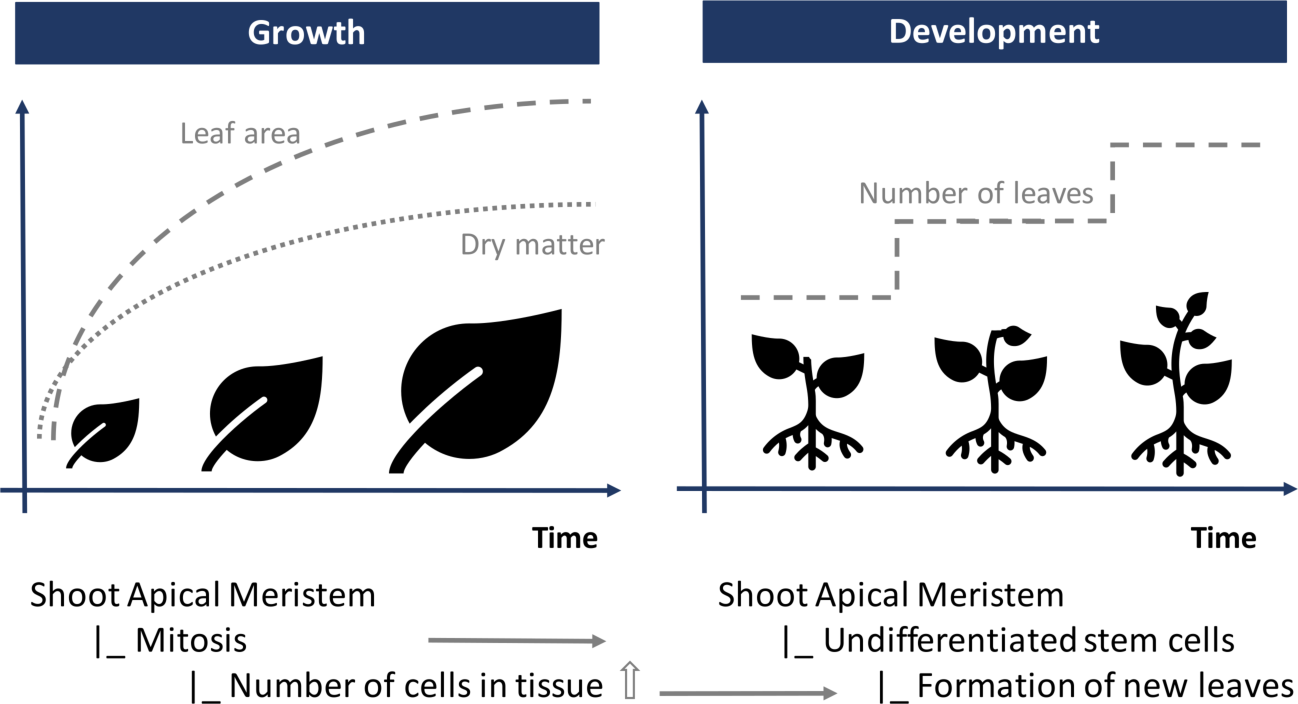
\includegraphics[width=\textwidth]{01-Introduction/img/growth_and_development.pdf}
    \caption{Illustrative example of leaf growth (left) by means of increasing leaf size and weight and plant development (right) by means of the appearance of new leaves from the main stem.}
    \label{fig:growth-development-biology}
\end{figure}

\subsection{Growth and development in winter wheat}

Winter wheat is an annual crop that uses the C3 photosynthetic pathway to fix atmospheric carbon. In the northern hemisphere, winter wheat is sown in the autumn (September to November in central Europe) and harvested in the summer (June to August) of the following year. Like all flowering plants, the development of winter wheat can be divided into a vegetative and a reproductive phase. To trigger this transistion, winter wheat requires vernalisation during the winter dormancy \citep{fedorov_photoperiodism_1976}, i.e. exposure to cold temperatures for a prolonged period.
Based on a growth-related perspective, \cite{kirby_analysis_1988} suggested to separate the growth and development process into three phases: The first phase consists of the formation of leaves and spikelets from the shoot apex. Following leaf development, tillers emerge from the axils of the leaves. This phases continues until the formation of the terminal spikelet and is followed by a vertical elongation of the stem and the ear. This second development stage finishes with the onset of anthesis. In the third and last stage growth and development are mainly confined to the grains.

Building on the three phases suggested by \cite{kirby_analysis_1988}, the focus is on winter growth and development in the first and second stage, i.e., between the formation of tillers (tillering) and the full emergence of the inflorescence (end of heading). % TODO: why this period? -> second phase important for yield!

Figure \ref{fig:ww-growth-development} shows winter wheat growth and development between the tillering (\gls{BBCH} 20 macro-stage) and heading stage (\gls{BBCH} 50 marco-stage) depicting three growth-related traits and their trajectory with progressing phenology.

\gls{GCC} (orange line in Figure \ref{fig:ww-growth-development}) exhibits the highest dynamic during tillering and stem elongation. It increases from values around 10 to 20\% during early tillering up to 80 or 85\% at the beginning of booting. Afterwards, \gls{GCC} shows a slight decreasing tendency. % does this match with the literature

\gls{GLAI} (green line in Figure \ref{fig:ww-growth-development}) shows a slightly delayed pattern compared to GCC. is low during the tillering phase and increases steadily until reaching a peak during early heading. Typically, \gls{GLAI} values in winter wheat can take up to 8 $m^2$ $m^{-2}$. After heading, \gls{GLAI} decreases as the onset of senescence means a decrease in chlorophyll.

Dry biomass is the only trait out of the three that shows a continuous increase from tillering to heading (purple line in Figure \ref{fig:ww-growth-development}).

\begin{figure}[H]
    \centering
    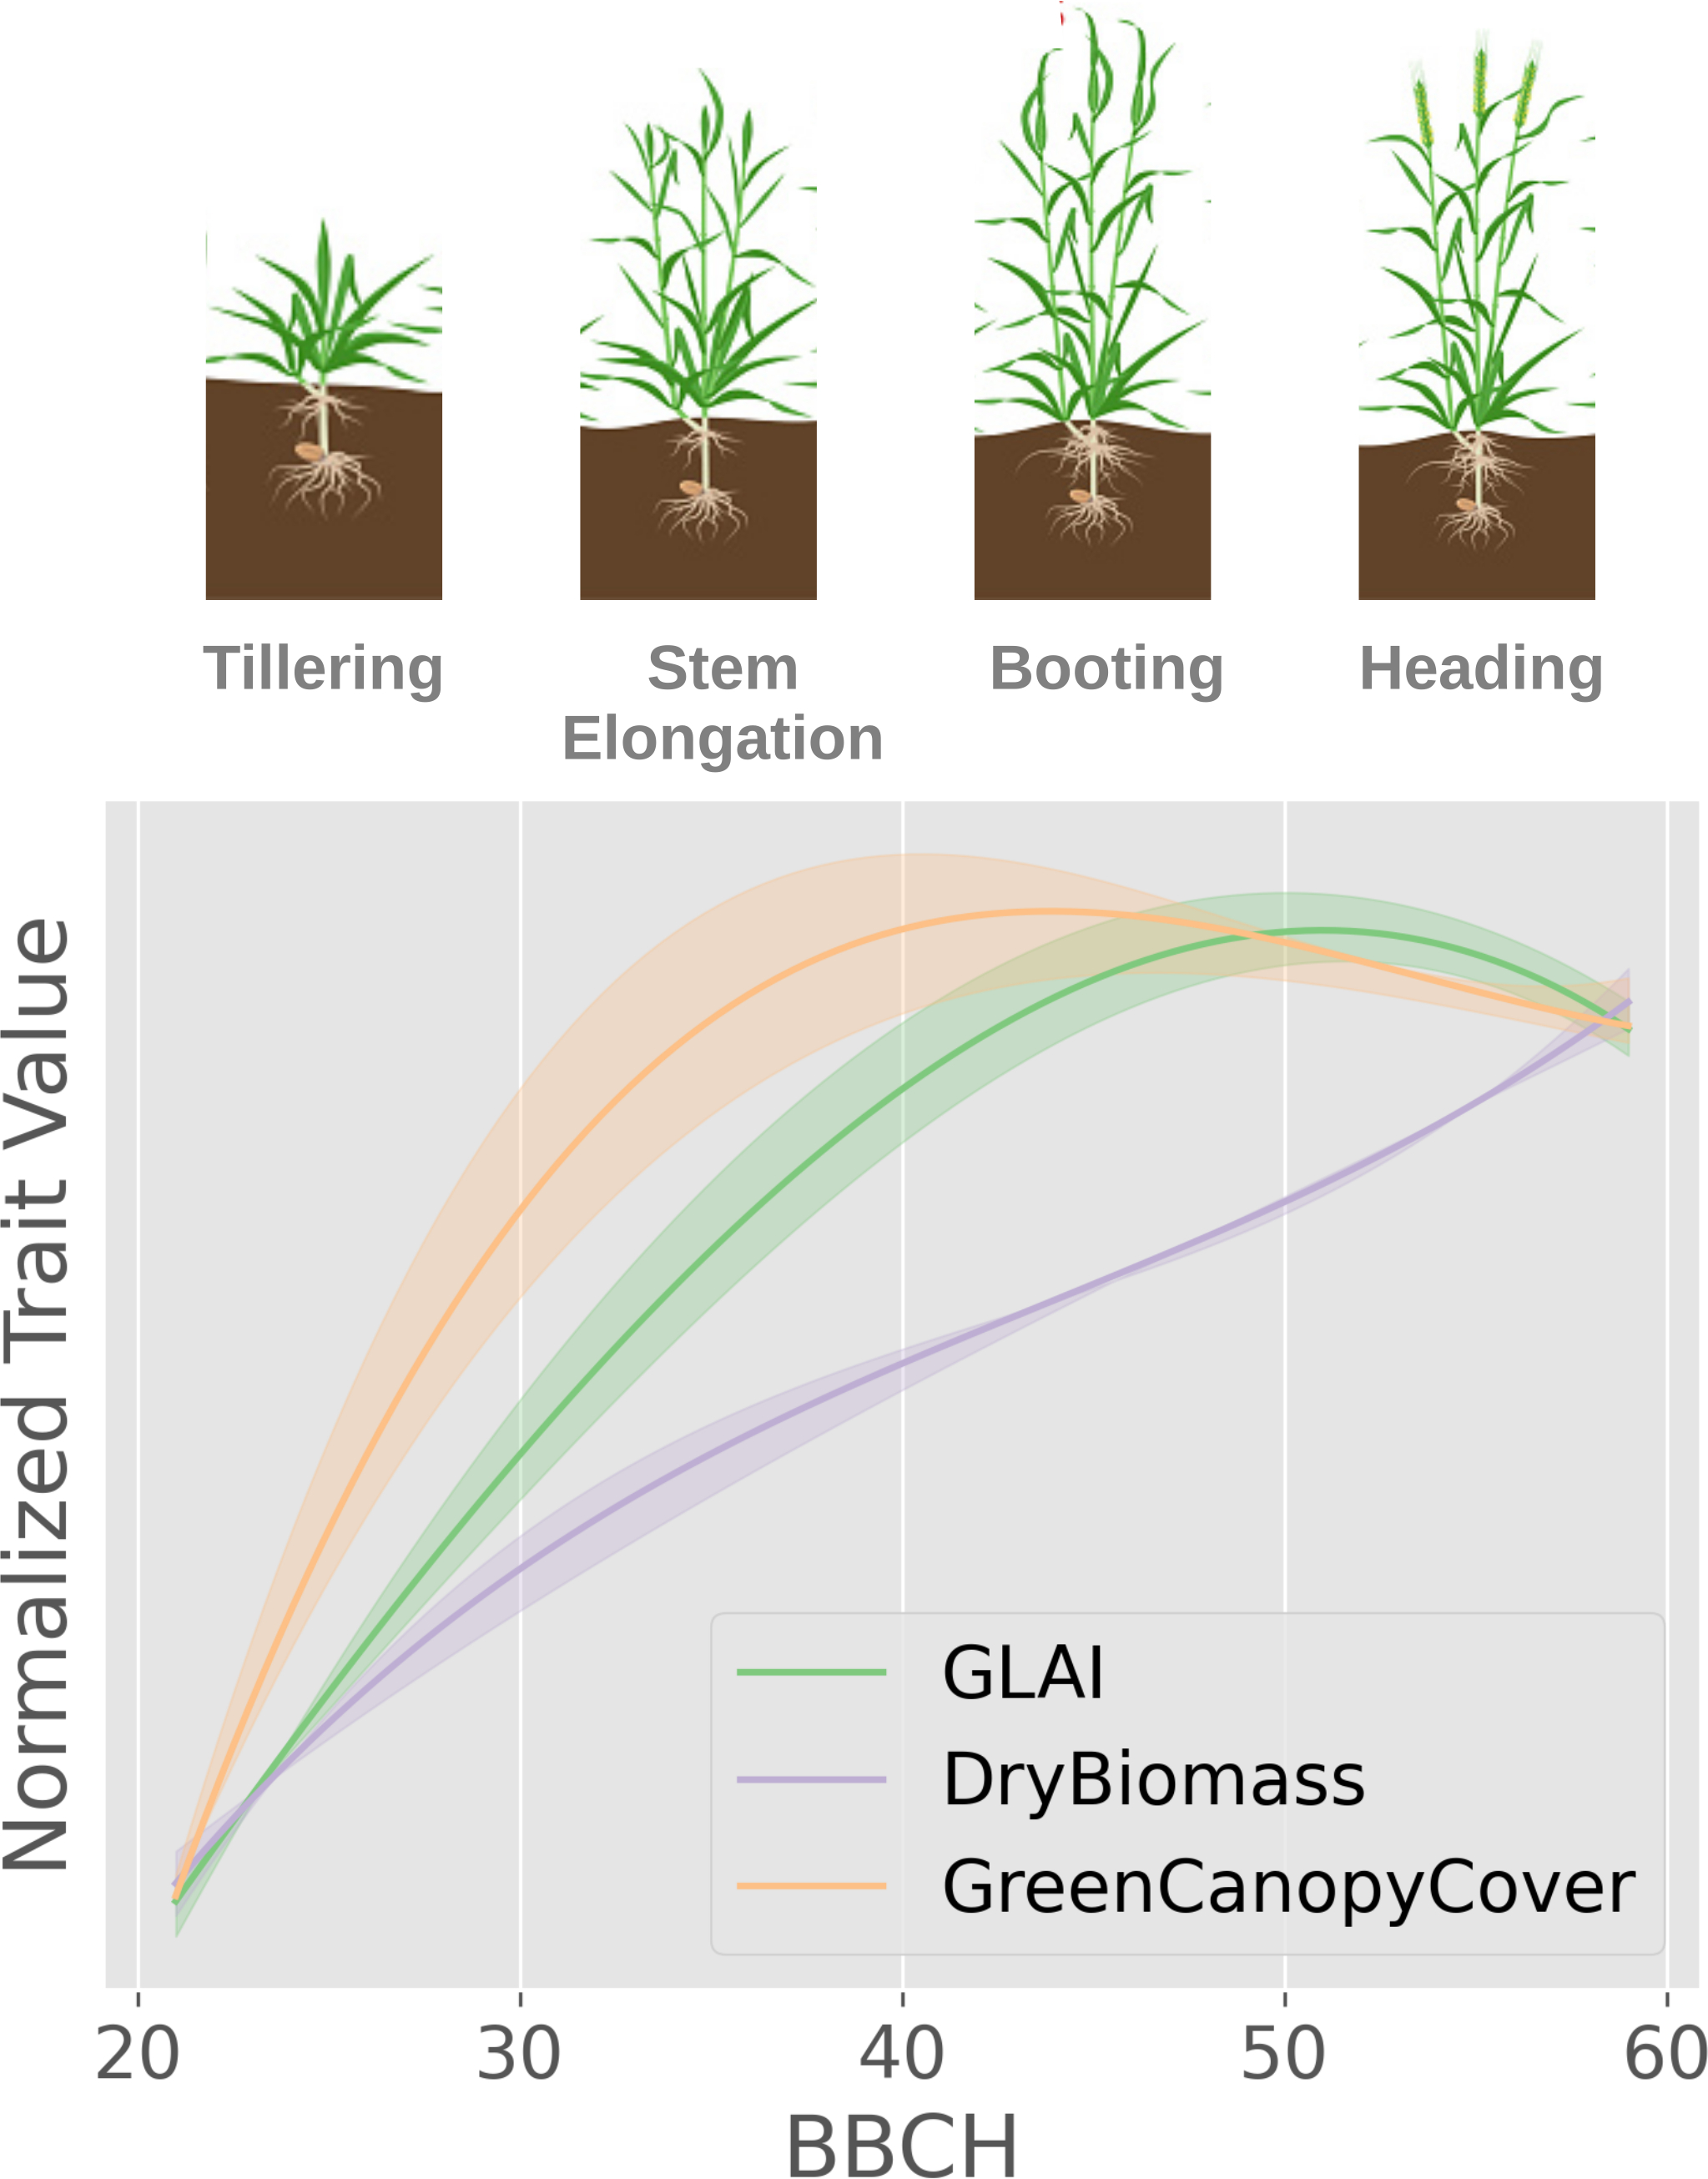
\includegraphics[width=\textwidth]{01-Introduction/img/figure_growth_and_development.jpeg}
    \caption{Growth and development in winter wheat between tillering and heading. The growth-related traits green leaf area index (GLAI, green), dry biomass (purple), and green canopy cover (orange) are plotted along the phenology axis expressed as BBCH growth stages. The trait values have been normalized between 0 and 1 to allow for a direct comparison.}
    \label{fig:ww-growth-development}
\end{figure}


\subsection{Field phenotyping, remote sensing and earth observation}

A key challenge is that the traits used in field phenotyping and remote sensing are often different and not necessarily compatible or interchangeable. Traits in field phenotyping often follow a physiological perspective on plant growth, such as \gls{DRC}s, while remotely sensed traits are often based on the ``traits-are-what-we-can-see'' principle, i.e. they are mostly spectral in nature, such as spectral indices \cite{bannari_review_1995} or absorption integrals \citep[for example]{wocher_rtm-based_2020}. As a result, coupling models from field phenotyping, such as complex mechanistic crop models and \gls{RTM} used in remote sensing, remains a challenge as model parameters are often incompatible, although some progress has been made \citep[for example]{thorp_estimating_2012}. There are also some terms that are defined or understood differently. For example, when the field phenotyping community refers to ``phenology'', they usually mean the timing of physiologically relevant transition phases in crop development, such as the onset of stem elongation in wheat. In the remote sensing community, however, ``phenology'' often refers to a change in spectral properties of crops, such as the increase in \gls{NDVI} after winter dormancy \citep{de_beurs_land_2004}.

% two disciplines that have similar aims but different approaches
% work on different scales, use different traits
% phenotyping traits: biological, physiological perspective
% remote sensing traits: focus on what we can see
% define EO as an umbrella term that might be better suited

% current methods in field phenotyping and RS
% highlight the missing link between field phenotyping and RS

\section{Objectives and research questions}

% How can we bridge field phenotyping and remote sensing using an EO approach?
% Can a combined approach out-perform "traditional" RS approaches?
% What are the (current) limitations and next steps and missing parts?

\section{Structure of the thesis}

This thesis is structured in six chapters excluding the Introduction.


\changelocaltocdepth{0} % only display the chapter level in the table of contents (TOC)

\chapter{EOdal: An Open-Source Python Package for Large-Scale Agroecological Research Using Earth Observation and Gridded Environmental Data}
\label{chap:eodal}
\graphicspath{{./02-EOdal/img}}

Lukas Valentin Graf\textsuperscript{1,2}, Gregor Perich\textsuperscript{1}, Helge Aasen\textsuperscript{1,2}
\\
\normalsize
\vspace{2pt}
\\
\textit{\textsuperscript{1}Group of Crop Science, Institute of Agricultural Sciences, Department of Environmental Systems Science, ETH Zurich, Universitätstrasse 2 , 8092 Zürich, Switzerland
\\
\textsuperscript{2}Earth Observation of Agroecosystems Team, Devision Agroecology and Environment,\ Agroscope, Reckenholzstrasse 191, CH-8042 Zürich, Switzerland
\vspace{2cm}}
\\

The following chapter contains a pre-print of the paper with the same title published in \textsl{Computers and Electronics in Agriculture} with the doi: \doi{10.1016/j.compag.2022.107487} under the Creative Commons Attribution License CC BY 4.0 (\url{http://creativecommons.org/licenses/by/4.0/}).

% the file
\section*{Abstract}
Earth Observation by means of remote sensing imagery and gridded environmental data opens tremendous opportunities for systematic capture, quantification and interpretation of plant - environment interactions through space and time. The acquisition, maintenance and processing of these data sources, however, requires a unified software framework for efficient and scalable integrated spatio-temporal analysis taking away the burden of data and file handling from the user. Existing software products either cover only parts of these requirements, exhibit a high degree of complexity, or are closed-source, which limits reproducibility of research. With the open-source Python library EOdal (Earth Observation Data Analysis Library) we propose a novel software that enables the development of fully reproducible spatial data science chains through the strict use of open-source developments.
Thanks to its modular design, EOdal enables advanced data warehousing especially for remote sensing data, sophisticated spatio-temporal analysis and intersection of different data sources, as well as nearly unlimited expandability through application programming interfaces (APIs).

\section{Introduction}
Images from \gls{EO} satellites and in-situ observations are of great importance for ecophysiological \citep{caparros-santiago_land_2021} and agroecological research \citep{karthikeyan_review_2020}. Such data can be used to determine plant traits and allow mapping of plant growing conditions for larger areas using standardized methods \citep{weiss_remote_2020}. Open-access, high-resolution satellite data such as from the European Space Agencies' \gls{S2} mission can resolve field heterogeneity and provide site-specific farming measures operationally. Examples include yield estimates \citep{marshall_optimizing_2018,perich_pixel-based_2023}, extraction of phenological metrics \citep{duarte_qphenometrics_2018}, variable irrigation rates \citep{barker_evaluation_2018} and site-specific fertilization scheduling \citep{mittermayer_analysis_2022}. Remotely sensed plant traits and their dynamic development over time  can further be augmented with environmental covariates such as climate, soil and terrain data, as well as information about farm management to perform integrated analysis on material and energy fluxes across spatio-temporal scales \citep{asam_relationship_2018}.

However, accessing, managing and analyzing \gls{EO} data is complex and often requires solid knowledge of geographic information science and coding to properly handle large spatial data sets. We base this finding on an exhaustive review of existing software tools. For example, the philosophy of the OpenDateCube \footnote{\url{https://www.opendatacube.org/}} initiative is about integrated analysis of \gls{EO} data using standardized interfaces. Installing the software, however, is complex as setting up a database instance is required. The Framework for Operational Radiometric Correction for Environmental monitoring (FORCE) \citep{frantz_forcelandsat_2019} is primarily designed for the creation of \gls{ARD} but does not provide interfaces for data analysis workflows. Analysis workflows using standardized interfaces are the main subject of the openEO\footnote{\url{https://openeo.org/}} project. openEO, however, focuses on cloud environments. Thus, data sets that are not available on externally operated web platforms are currently excluded. This applies particularly to (experimental) research data sets. Researchers therefore often spend a significant amount of time getting the data into an analysis-ready format. Based on the analysis of more than 3000 productive machine learning pipelines at Google, \citet{xin_production_2021} identified great potential for optimization in the area of data management and pre-processing, which also appears to be true in the \gls{EO} area.

For these reasons, we developed the \gls{EOdal} as an open-source Python (3.8+) package designed to make \gls{EO} data analysis tools available to researchers without the need for in-depth knowledge about geoinformation science, coding and remote sensing data handling. A key aspect of \gls{EOdal} is the ability to apply spatial data science methods to data from different sources within a unified framework based on open-source tools. We also intend to provide researchers with an alternative to proprietary software solutions such as the widely used Google Earth Engine \citep{gorelick_google_2017}.

The functionality and structure of \gls{EOdal} is explained in Section \ref{sec:package_struc} of this paper. In Section \ref{sec:reprod_example}, we present a reproducible use case based on an agricultural research question followed by a discussion in Section \ref{sec:eodal_conclusions}.

\section{Description of EOdal}
\label{sec:package_struc}
\gls{EOdal} consists of three layers as shown in Figure \ref{fig:overview}. The layers are organized in a triangle to emphasize their inter-dependencies. The core layer (Figure \ref{fig:overview}, top) provides the Python classes required to perform I/O operations to read and write geo-spatial data sets in a generic way. It is also the basis for data warehousing, i.e., the storage of metadata. Class inheritance extends its capabilities to specific \gls{EO} sensors such as \gls{S2} Multispectral Imager (e.g., for convenient reading of data organized in the Satellite Archive for Europe structure). (Pre-)processing of these datasets is accomplished in the processing layer (Figure \ref{fig:overview}, lower right). Processing steps such as spatial reprojection are often a necessity to combine different datasets for analysis. The analysis layer (Figure \ref{fig:overview}, lower left) enables automatized, reproducible \gls{EO} data management and is the backbone for data-driven analysis of geo-spatial data sets and their spatio-temporal intersection.

Deployment of \gls{EOdal} is independent of an Operating System. Furthermore, \gls{EOdal} can be used on local premises (e.g. for processing research datasets) but also in cloud environments for fast access to large, freely accessible data such as the global \gls{S2} or Landsat archive. To enable fast and scalable deployment required for large-scale analysis tasks \gls{EOdal} can be installed into containerized environments (Docker containers).

\subsection{Core Layer}
The data model of the core layer (Figure \ref{fig:overview} top) follows the object-oriented programming paradigm and includes different classes. There are three classes in the \gls{EOdal} core layer: Bands, RasterCollections and derived (inherited) sensor-specific classes. The Band class represents the base class. In simple terms, a Band refers to a two-dimensional array referenced in a geo-spatial coordinate reference system. A RasterCollection is a collection of zero to $n$ Band objects, which can exist in different spatial reference systems, grid cell sizes (pixel sizes) and spatial extents. Band objects in a collection are identified by names (e.g., "blue", Figure \ref{fig:overview} top right) instead of numeric indices. Bands and RasterCollections can be created from any geo-referenced raster data set understood by Geospatial Data Abstraction Library (GDAL, e.g., GeoTiff), vector features (e.g. Shapefile, GeoJSON), and from numerical arrays (Python libraries, e.g. NumPy, Zarr). Sensor-specific RasterCollections include all the functionalities and attributes of the RasterCollection class, but are tailored to the requirements and capabilities of specific imaging sensors such as, for example, \gls{S2}, or Landsat. The inheritance-based software design allows the introduction of further sensors and makes the core layer extensible also with regard to upcoming future \gls{EO} platforms such as the hyperspectral Copernicus expansion mission CHIME\footnote{\url{https://www.esa.int/Applications/Observing_the_Earth/Copernicus/Going_hyperspectral_for_CHIME}} and beyond.

A further central element of the core layer is the collection of metadata in a spatio-temporal catalog  allowing the filtering of records by data source, time period, and geographic region of interest (ROI). \gls{EOdal} supports \gls{STAC}, which are available in many cloud environments that provide geo-spatial (satellite) data, such as Microsoft Azures Planetary Computer\footnote{\url{https://planetarycomputer.microsoft.com/}}, Amazon Web Services (AWS) Earth\footnote{\url{https://aws.amazon.com/de/earth/}} and the Copernicus Data and Information Access Services (DIAS). For local deployment, \gls{EOdal} offers the possibility to store metadata in a PostgreSQL database with the spatial PostGIS extension.

In terms of spatial data models and standards, \gls{EOdal} supports area (polygons and multi-polygons) as well as point features following the general feature model defined in the ISO 19109 standard \citep{iso_iso_2015}. This allows point-based in-situ observations, for example from weather stations or ground sensors, to be intersected with \gls{EO} data and auxiliary data sources such as Digital Elevation Models (see Section \ref{sec:reprod_example}).

\subsection{Processing Layer}
\label{subsec:processing-layer}
The processing layer (Figure \ref{fig:overview}, lower right) provides functionalities for \gls{EO} data preparation and (pre-)processing. Data preparation is usually necessary to enable the merging datasets from different sensors and platforms. This includes image manipulation methods such as spatial resampling and reprojection from one coordinate system into another or masking operations to mask out bad quality observations or land cover classes.

\subsection{Analysis Layer}
The analysis layer (Figure \ref{fig:overview}, bottom) is used for the analysis of data from \gls{EO} satellites and environmental covariates such as meteorological, terrain, soil and land use data. It builds upon the core layer to query and access different data sources and the processing layer to prepare the data analysis-ready. The underlying complex data management such as the merging of data from satellite tiles and filling of no-data values is hidden from the user in the processing layer (see Section \ref{subsec:processing-layer}).

\gls{EOdal} provides interfaces to widely-used open-source Python libraries (e.g., geopandas, numpy, xarray). This allows users to integrate their own \gls{EO} processing workflows and modules (c.f. section \ref{subsec:supplementary-modules}) to e.g. estimate biochemical, structural or integrated traits such as chlorophyll, leaf area index, yield or land surface phenology (Figure \ref{fig:overview}, lower left). 

\subsection{Applications of EOdal}
\label{subsec:supplementary-modules}
\gls{EOdal} has already been used for studies in agroecological research. \citet{perich_pixel-based_2023} used \gls{EOdal} for pixel-based prediction of crop yield using S2 time series.  In \citet{graf_propagating_2022}, \gls{EOdal} is used to propagate radiometric uncertainty from \gls{S2} reflectance factors to phenological metrics. Moreover, \gls{EOdal} drives the \gls{EO} platform at the Swiss Federal Center of Excellence for Agricultural Research, Agroscope, underpinning its relevance within an operational and governmental environment\footnote{\url{http://www.eoa-team.net/}}.

\begin{figure}[H]
    \centering
    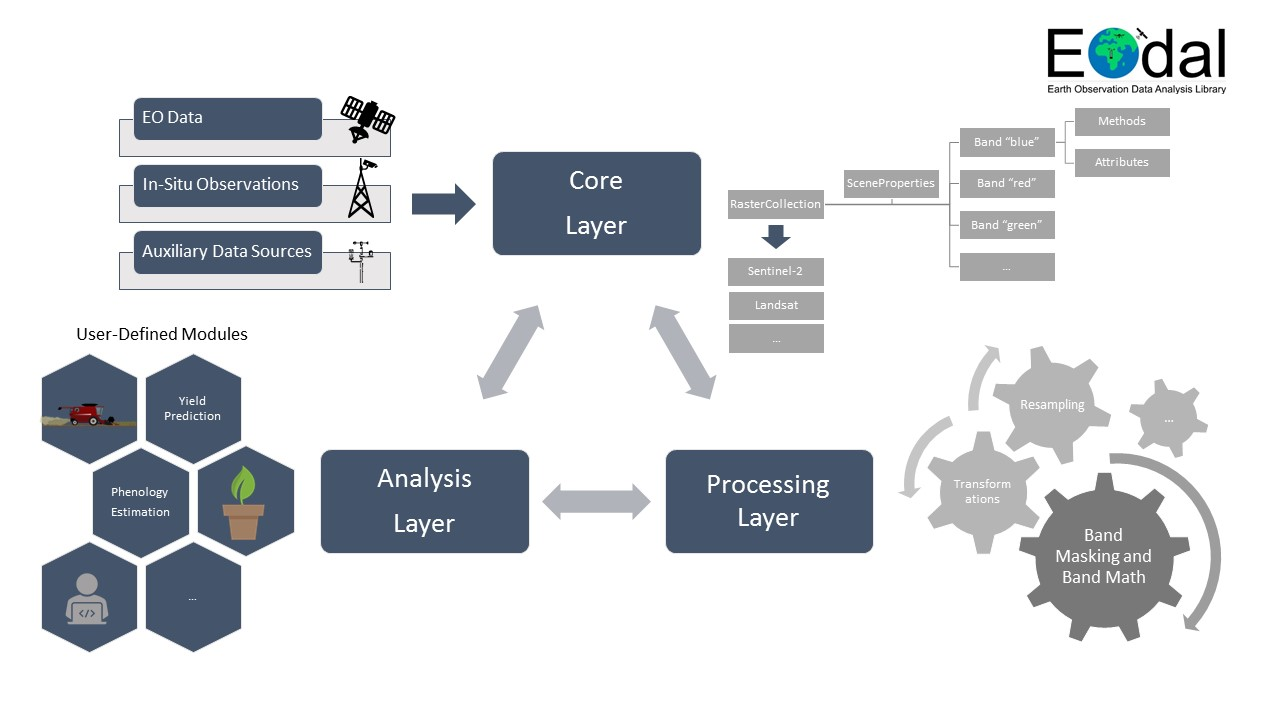
\includegraphics[width=\textwidth]{EOdal_layers.jpg}
    \caption{Overview of EOdal and its three layers: The core layer (top) handles different input data sources in a standardized way. The analysis layer (bottom left) builds upon the core and the processing layer (bottom right) for data maintenance, querying, intersection and integration into user-defined data science pipelines.}
    \label{fig:overview}
\end{figure}

\section{Usage Example: Interpreting In-Field Growth Heterogeneity Through Time with Topographic and Meteorological Data}
\label{sec:reprod_example}
We illustrate here the potential of EOdal for integrated spatio-temporal analysis over an example ROI from western Switzerland near Lake Neuchâtel ($46.98^\circ N$, $7.07^\circ E$). All results were produced by a single Jupyter notebook (\url{https://doi.org/10.1016/j.compag.2022.107487}) running \gls{EOdal} v0.0.1 on Microsoft Planetary Computer. Due to large-scale land subsidence, the entire region - a former peat land - is subject to increased flood risk \citep{egli_landschaftsdynamik_2020}. An agricultural parcel (12 ha) was affected by flooding during heavy rainfall (360 mm within 30 days) between mid-June and July 2021, causing flood damage to the previously homogeneous green canopy. Figure \ref{fig:s2-fig} shows \gls{S2} derived false-color infra-red images of the parcel in 2021 before the flood (reddish tones in Figure \ref{fig:s2-fig}a). In the spring 2022, differences in canopy greenness of the emerging winter wheat are evident (Figure \ref{fig:s2-fig}b and c). Darker areas, which indicate lower soil cover, can be discerned in the otherwise red-colored canopy. The spatial pattern within the field corresponds to the patterns within the DEM (Figure \ref{fig:s2-fig}e) and reveals that parts with lower elevation values were more impacted by flooding than the rest of the field. Extraction of the Modified Soil Adjusted Vegetation Index (MSAVI, \cite{qi_modified_1994}) time series from two selected S2 pixels (Figure \ref{fig:s2-fig}d) allows to evaluate the impact of the flood in 2021 on the growth dynamic in 2022 and confirms the findings from the false-color S2 images.
As additional usage example, the growth pattern of a field is investigated in relation to meteorological data, often used to validate and calibrate ecophysiological growth models. In this case (Figure \ref{fig:s2-fig}f), the cumulative growing degree days (in °C) and cumulative daily rainfall amount (in mm) were derived from a nearby weather station (Ins) operated by the Swiss Federal Office of Meteorology and Climatology (MeteoSwiss) calculated from November \nth{1} 2021.

\begin{figure}[H]
    \centering
    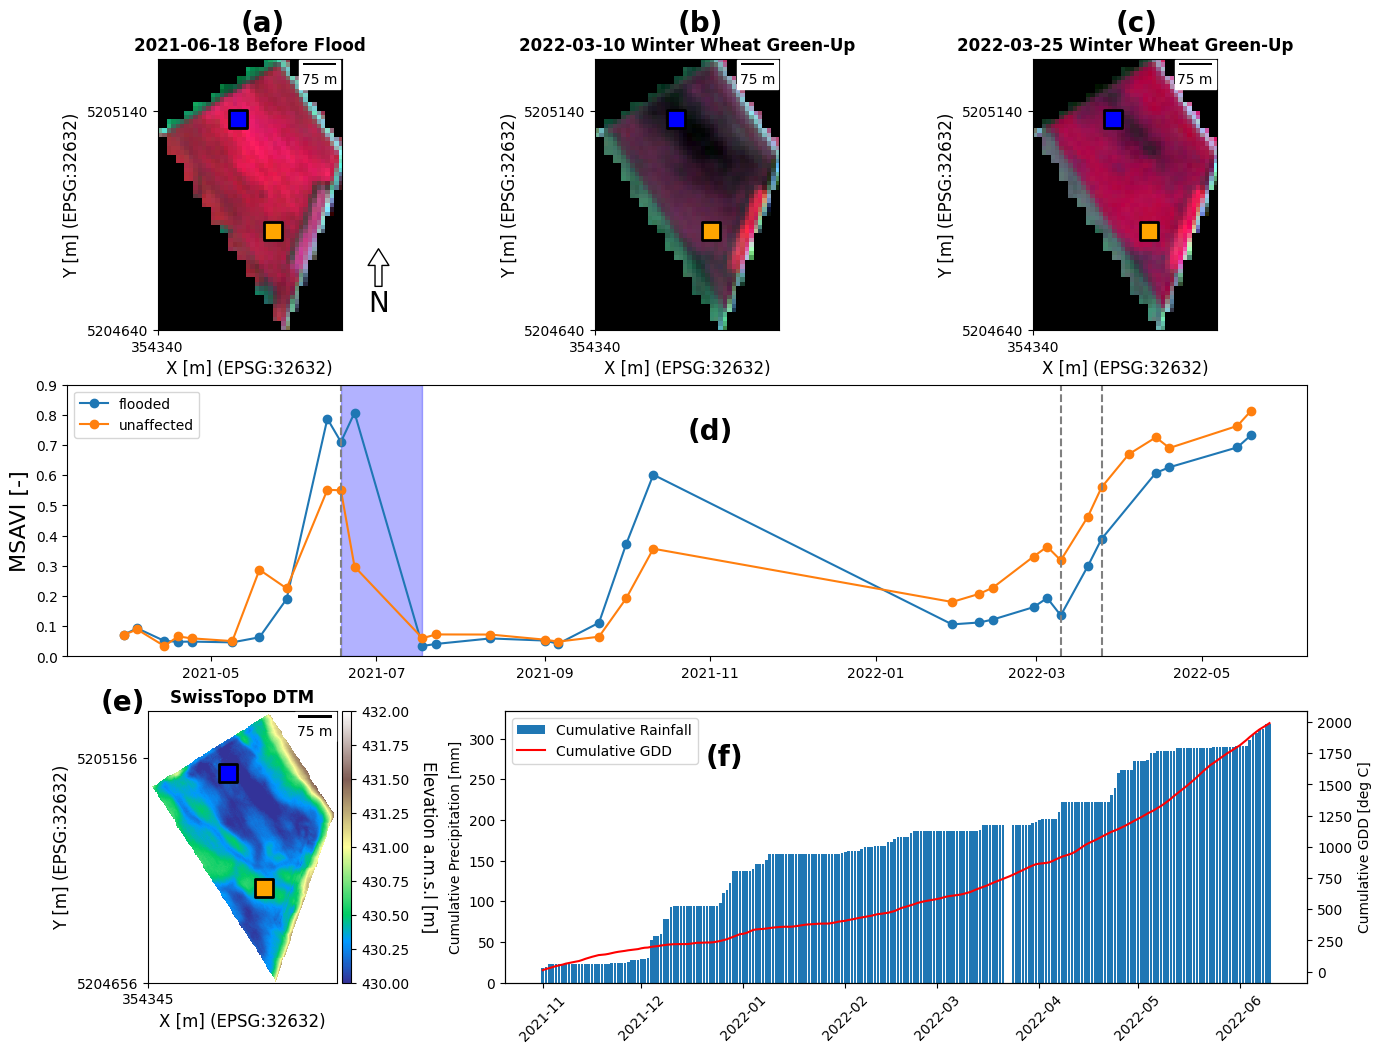
\includegraphics[width=\textwidth]{S2_Flood_Crop_Growth_Example.png}
    \caption{Result of a single Jupyter notebook run using \gls{EOdal} (v0.0.1) on Microsoft Planetary Computer. \gls{S2} false-color infra-red composite of the field parcel before the heavy rainfall events in June and July 2021 (a) and spatial heterogeneity in winter wheat green-up during spring 2022 (b-c). In addition, cumulative growing degree days (GDD) and daily precipitation sums derived from a nearby weather station are shown (f). The extent of the flood in 2021 - evident as darker areas in (b-c) - corresponds to a depression visible in the Digital Elevation Model (e). The flood affected plant growing conditions in spring 2022 as shown in the MSAVI time series (d) of a 'flooded' pixel (blue) and a pixel that was little affected by the floods in 2021 (orange). The dashed lines in (d) correspond to the timing of (a), (b) and (c), respectively, whereas the blue rectangle in (d) indicates the approximate timing of the flooding in 2021.}
    \label{fig:s2-fig}
\end{figure}

\section{Discussion and Conclusion}
\label{sec:eodal_conclusions}
%\chapter{General discussion}
\label{chap:general-discussion}

The aim of this chapter is to bring together the different aspects of the research carried out (Chapters \ref{chap:eodal}-\ref{chap:drc}) within the framework of a landscape-scale prototype and to discuss its applications, limitations and possible further research questions. However, the scientific discussion of the individual research chapters is not repeated here. Please refer to the relevant discussion subsections in the previous chapters.

\section{A prototype for landscape-scale phenotyping}
Figure \ref{fig:oa-disc-prototype} shows a sketch of how the individual research components can be transferred to a landscape level prototype to quantify winter wheat growth and development.

The main data sources for the prototype are environmental covariates, mainly air temperature, and high resolution optical satellite imagery from the \gls{S2} mission. The necessary calibration of the prototype is mainly based on field phenotyping data, which encode the relationships between development and growth (see chapter \ref{chap:insights}) and establish the relationship between plant growth and environmental conditions (chapter \ref{chap:drc}). These calibration data thus represent the physiological and phenological knowledge of G $\times$ E interactions in crops in general and wheat in particular.

Using the calibration and the two data sources, the functionality of the prototype can now be demonstrated in three steps.

\paragraph{Step 1 -- Timing and duration of key phenological stages}
The first step is to determine the timing of key phenological development stages as described in Chapters \ref{chap:phemology} and \ref{chap:insights}. This is important to determine the onset and duration of the \gls{SE} period, which is the focus of attention due to its importance in grain yield formation, as explained in Chapter \ref{chap:introduction}. The phenology model uses only weather data and has a relatively coarse spatial resolution (km scale) due to the relatively coarse resolution of most meteorological data products at the landscape scale. The timing extracted from the phenology model will therefore limit the period over which satellite data should be considered.

\paragraph{Step 2 -- Trait retrieval from satellite imagery}
Once the relevant time period has been extracted, satellite data are searched and converted to \gls{GLAI} using physiological and phenological priors from field phenotyping as described in Chapter \ref{chap:insights} using RTM inversion and the software \gls{EOdal} (Chapter \ref{chap:eodal}). Thus, at $n$ time points, where $n$ is the number of \gls{S2} scenes, \gls{GLAI} estimates are available at 10 $\times$ 10 m spatial resolution. This allows spatial detail to be resolved, e.g. on within-field heterogeneity, which is not available from the temperature data. The \gls{GLAI} estimates based on the \gls{S2} data are thus snapshots of the apparent growth conditions.

\paragraph{Step 3 -- Reconstruction of growth}
Using the \gls{S2} \gls{GLAI} observations and the air temperature data, the growth dynamics in the \gls{SE} period can be modelled in hourly or daily resolution in a final step, as described in Chapter \ref{chap:drc} using \gls{DRC}s. In this way, the high temporal resolution of the temperature data is combined with the spatial detail of the \gls{S2} \gls{GLAI} observations. Here, not only the physiological knowledge from the field phenotyping is encoded, but also the uncertainty propagation carried out in Chapter \ref{chap:uncertainty} is used to model growth and development during the \gls{SE} period.

\begin{figure}[H]
    \centering
    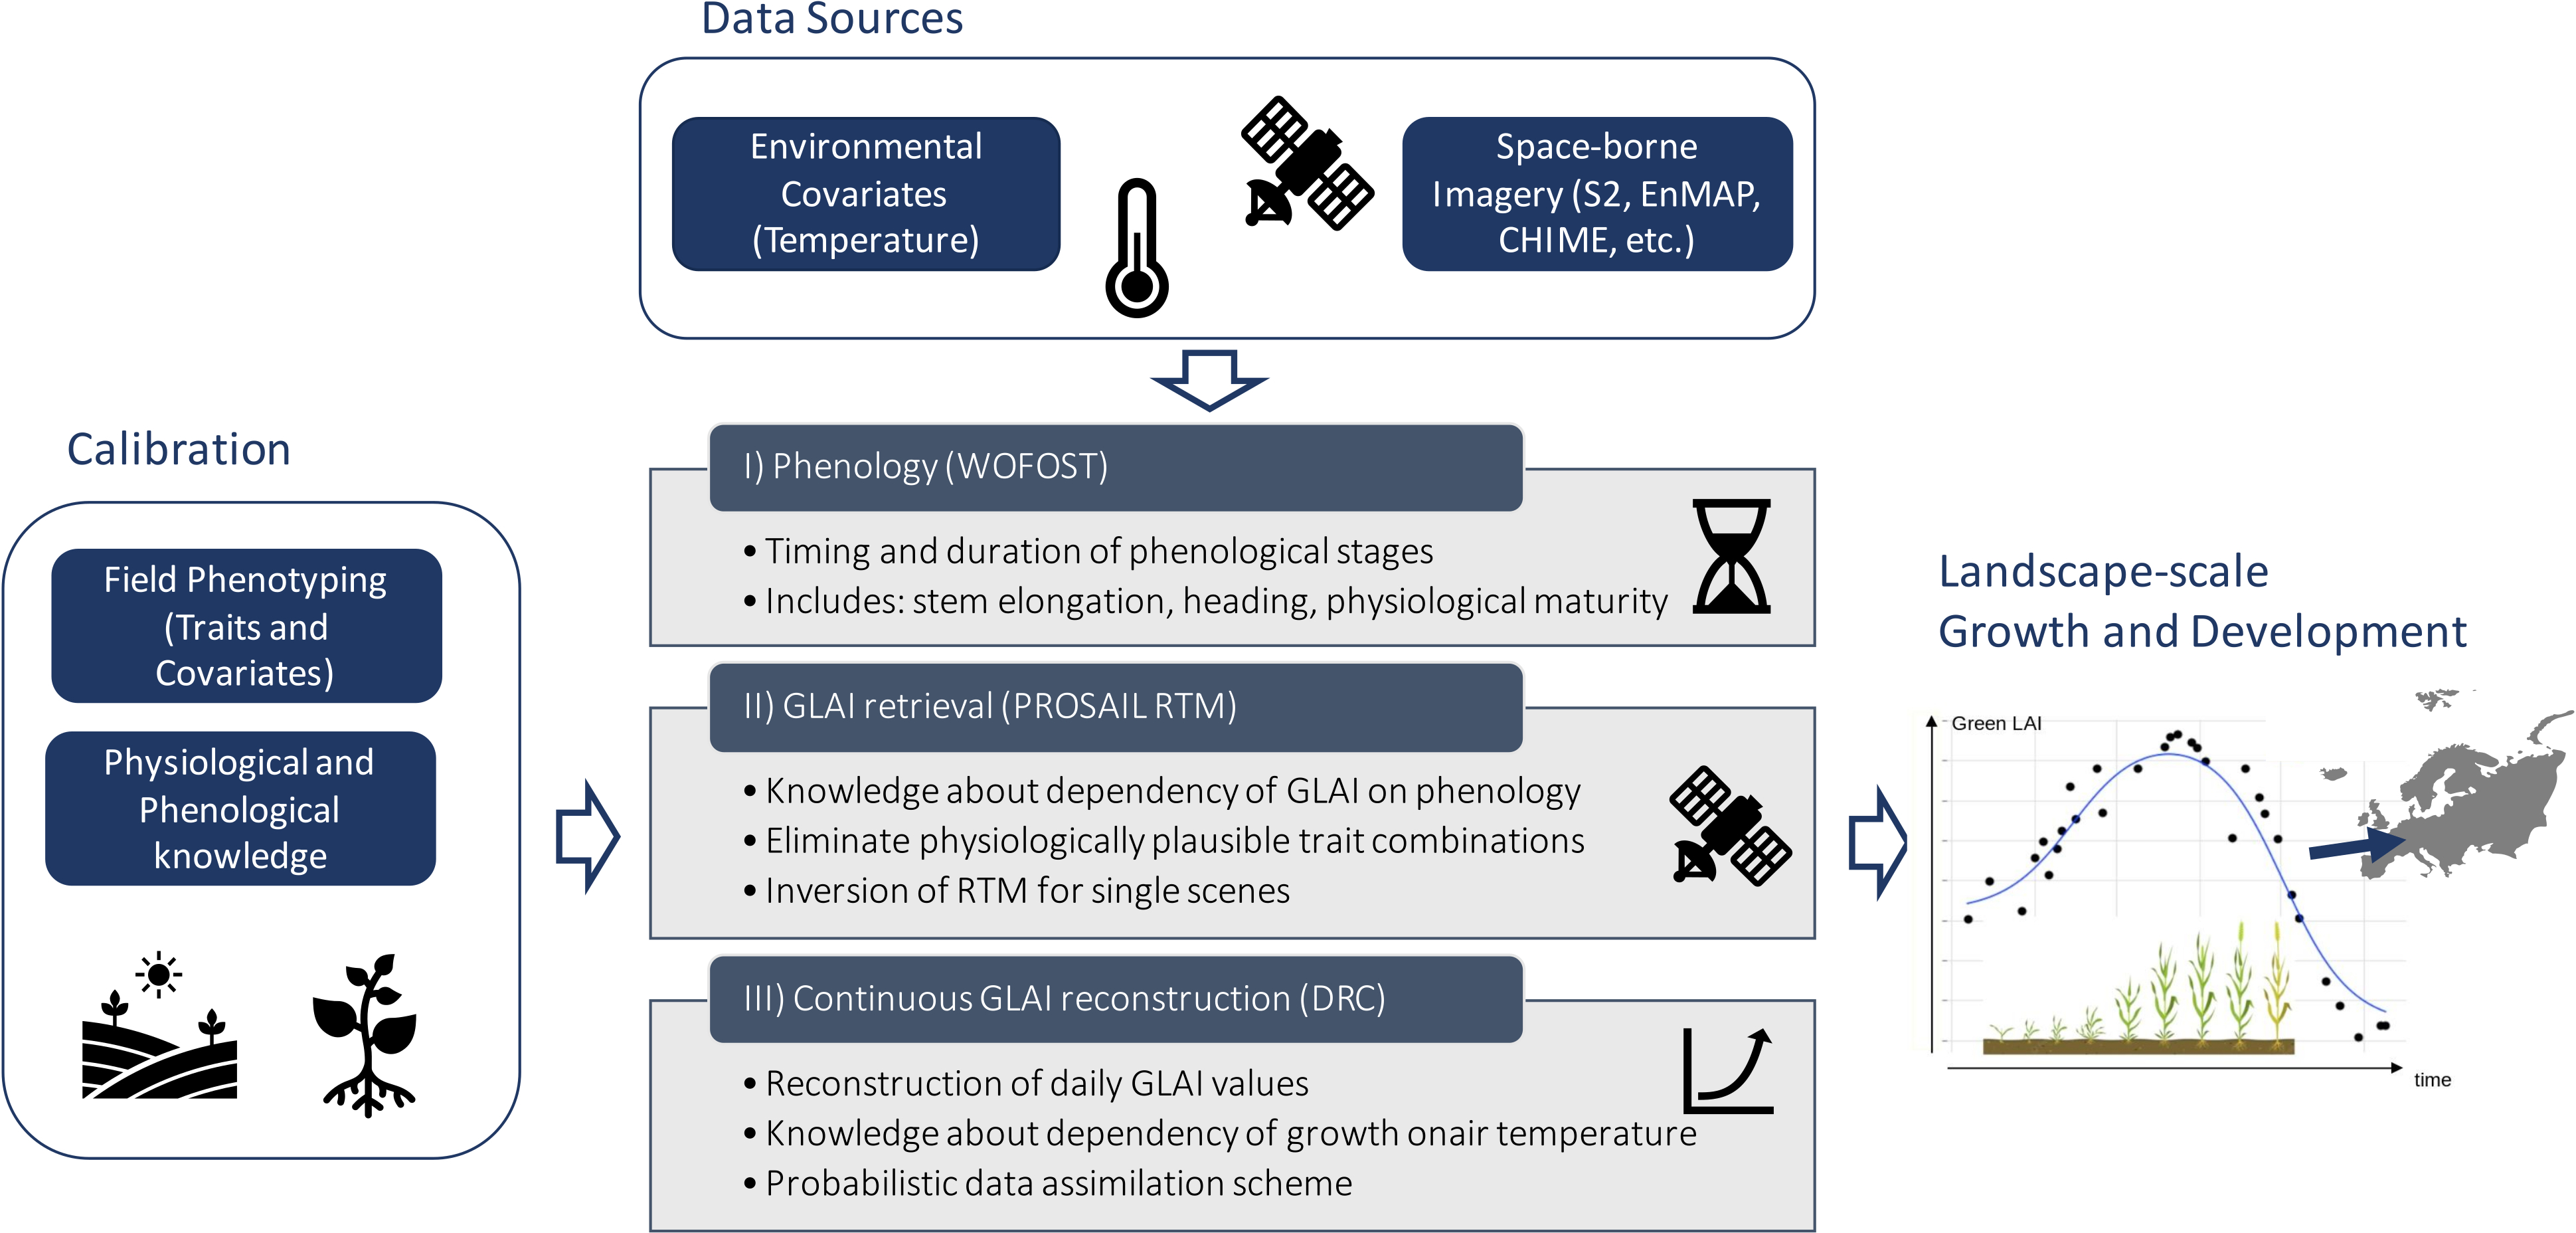
\includegraphics[width=\textwidth]{07-Discussion/img/prototype.jpg}
    \caption{The proposed prototype for landscape scale phenotyping of winter wheat growth and development as a key outcome of this thesis.}
    \label{fig:oa-disc-prototype}
\end{figure}

The prototype composed of these components thus allows the quantification of winter wheat growth and development at the landscape scale, for example in the Swiss Mittelland, with a spatial resolution of up to 10 m and a temporal resolution of up to one hour. Furthermore, by combining satellite, meteorological and in-situ data, the prototype can be considered as a true \gls{EO} system. At the same time, the quantification of growth through \gls{GLAI} values and development through phenological stages means that the prototype is also a phenotyping system. Overall, the prototype presented is in line with multilateral incentives such as \gls{GEOCLAM} that aim to provide traceable, actionable insights to stakeholders in agriculture \citep{whitcraft_no_2019}. As the prototype relies on open satellite and, at least in most cases, readily available temperature data and rather simple but physiologically meaningful models, it appears well suited for further operationalisation and near-realtime deployment.

\section{Answers to research questions}
With the prototype (Figure \ref{fig:oa-disc-prototype}) the three research questions outlined in section \ref{sec:intro-obj-rj} can be addressed.

\subsection{How can field phenotyping and spaceborne remote sensing data be combined to allow up-scaling of physiological knowledge from field phenotyping to the landscape-scale?}
This thesis has identified two ways of combining field phenotyping and spaceborne remote sensing data. The first way is to use field phenotyping data as prior knowledge to constrain \gls{RTM} simulations as shown in chapter \ref{chap:insights}, and to fill temporal gaps and remove outliers using \gls{DRC}s to reconstruct hourly or daily \gls{GLAI} trajectories from single \gls{S2} observations (Chapter \ref{chap:drc}). While the first way directly addresses the workflow of remote sensing retrieval and time series reconstruction, the second way is about using field phenotyping data to parameterise phenological models (Chapter \ref{chap:phemology}), which in turn are used to select relevant satellite imagery and quantify the timing of key developmental stages such as the end of heading. It is thus a more indirect way of incorporating field phenotyping data into an \gls{EO} approach. As a result, both pathways allow knowledge and concepts to be scaled up from field phenotyping to the landscape scale.

\subsection{Can a landscape-scale phenotyping approach provide accurate, physiologically based and traceable insights into winter wheat growth and development?}
The quantification of uncertainties (see Chapter \ref{chap:uncertainty}) fulfils the requirement for traceability (Section \ref{sec:intro-obj-rj}). The integration of prior knowledge from field phenotyping into the \gls{GLAI} retrieval process in step 2, as well as into the parameterisation of \gls{DRC}s in step 3, fulfils the requirement for physiological plausibility (see also the individual scientific discussions in Sections \ref{sec:insights_discussion} and \ref{sec:drc_discussion}). The accuracy of the methodology has been demonstrated using multi-year, independent in-situ data for phenological development (RMSE for heading date: 2 days, Chapter \ref{chap:phemology}) and GLAI (smallest relative error: 13\%, Chapter \ref{chap:drc}). This research question can therefore be answered in the affirmative.

\subsection{What are the potentials but also the limitations and challenges of such a landscape phenotyping approach?}

The prototype allows the study of G $\times$ E interactions that could not be fully addressed by small-scale field phenotyping experiments. These include effects of changes in soil properties or topography that are spatially continuous and affect plant growth and development through soil water availability, exposure to wind and sunlight, or nutrient availability. In addition, the \gls{GLAI} estimates can be converted to biomass \citep{aase_relationship_1978} and -- in perspective -- grain yield, which are arguably important agronomic traits for decision making and policy advice. Accurate modelling of these traits will therefore not only advance the science behind \gls{EO}-based applications for agriculture, but also help to meet the needs of a growing world population.


% lack of further calibration data
% lack of management data -> varieties (paper dario with share of varieties); sowing date lacking
% scalability: that's a core promise of RS but holds only true for the radiative properties; the translation into traits is more difficult!

\section{Open questions}
\subsection{Spatial or temporal detail?}

\subsection{What are the limiting factors?}
% we worked with temperature, only!
% the questions is: what are the limiting factors of growth and development
% do not forget about the management!

\section{Outlook}
% extend to senescence phase -> grain filling phase
% different crops -> other cereals but also pulses, etc.
% include different RS data sources (Planet, S1, etc.)
% methodology
The usage example shown in Figure \ref{fig:s2-fig} highlights how \gls{EOdal} can be used to combine different environmental covariates with vegetation dynamics obtained from satellite time series to develop a holistic understanding of plant-environment interactions. This simple example shows how \gls{EOdal} lowers the barriers of entry to \gls{EO} analysis unlocking potential for data-based decision-making in agroecology. In addition, by using Docker and cloud infrastructure, the analysis can be extended to larger spatial and temporal scales. For the future we envision an ecosystem of user modules that build on EOdal, complement themselves and are developed and made freely available to the \gls{EO} community. 

\gls{EOdal} is in line with recent developments in agriculture that allow (technically inexperienced) users to run complex analyses: \citet{godara_agrimine_2022} developed a platform called "AgriMine". The platform enables spatio-temporal analysis of issues in Indian agriculture based on help-desk calls improving the Indian agricultural extension service. Improvements in variety testing were enabled by an online platform in China that makes processes more efficient and lines up with recent incentives in high-throughput phenotyping efforts \citep{pan_online_2022}. Similarly, \gls{EOdal} can contribute to increased use of EO data in agriculture.

Although we focus on agriculture (section \ref{subsec:supplementary-modules}), \gls{EOdal} is not limited to it. Rather, EOdal can be used in all disciplines that process \gls{EO} data and require open, reproducible data analysis workflows. Thus, we expect EOdal to trigger further open-source developments, either through the release of additional Python packages that build on the existing functionalities, or through its integration into existing data processing frameworks. Ultimately, \gls{EOdal} is intended to provide researchers with an alternative to proprietary software platforms while also easing the burden of data management for practitioners. For this reason EOdal is particularly well suitable for educational activities in the field of \gls{EO}. This supports the transition to reproducible science, benefiting the \gls{EO} community as a whole.

\section*{CRediT Authorship Contribution Statement}
Lukas Valentin Graf: Conceptualization, Software, Investigation, Visualization, Writing – original draft, Writing – review \& editing. Gregor Perich: Conceptualization, Software, Writing – original draft, Writing – review \& editing. Helge Aasen: Supervision, Writing – original draft, Writing – review \& editing.

\section*{Declaration of Competing Interest}
The authors declare that they have no known competing financial interests or personal relationships that could have appeared to influence the work reported in this paper.

%% create a non-numbered section for the Acknowledgements
\section*{Acknowledgements}
The authors thank Achim Walter from the Crop Science group at ETH for providing the IT infrastructure and in particular Norbert Kirchgessner for his support with data storage and implementation. Furthermore, we thank Alfred Burri for on-site support and contributions to the usage example and Fabio Oriani for valuable comments on the manuscript. The development of EOdal was conducted within the project `PhenomEn' funded by the Swiss Science Foundation (grant number IZCOZ0\_198091). GP acknowledges funding through the project `DeepField' of the Swiss Federal Office for Agriculture (BLW). 

\newpage % for fancy formatting

\chapter{Insights from field phenotyping improve satellite remote sensing based in-season estimation of winter wheat growth and phenology}
\label{chap:eodal}
\graphicspath{{./05-Insights/img}}

Lukas Valentin Graf\textsuperscript{1,2}, Quirina Noëmi Merz\textsuperscript{1}, Achim Walter\textsuperscript{1}, Helge Aasen\textsuperscript{1,2}
\\
\normalsize
\vspace{2pt}
\\
\textit{\textsuperscript{1}Group of Crop Science, Institute of Agricultural Sciences, Department of Environmental Systems Science, ETH Zurich, Universitätstrasse 2 , 8092 Zurich, Switzerland
\\
\textsuperscript{2}Earth Observation of Agroecosystems Team, Devision Agroecology and Environment,\ Agroscope, Reckenholzstrasse 191, CH-8042 Zürich, Switzerland
\vspace{2cm}}
\\

The following chapter contains a re-print of the paper with the same title published in \textsl{Remote Sensing of Environment} with the doi: \doi{10.1016/j.rse.2023.113860} under the Creative Commons Attribution License CC BY 4.0 (\url{http://creativecommons.org/licenses/by/4.0/}).

% the file
\section*{Abstract}
Timely knowledge of phenological development and crop growth is pivotal for evidence-based decision making in agriculture. We propose a near real-time approach combining radiative transfer model inversion with physiological and phenological priors from multi-year field phenotyping. Our approach allows to retrieve Green Leaf Area Index (GLAI), Canopy Chlorophyll Content (CCC) and hence Leaf Chlorophyll Content (Cab) from Sentinel-2 optical satellite imagery to quantify winter wheat growth conditions in a physiologically sound way. Phenological macro stages are based on accumulated growing degree day thresholds obtained from multi-year field phenotyping covering more than 2400 ratings from roughly 300 winter wheat varieties and reflect important physiological transitions. These include the transition from vegetative to reproductive growth and the onset of flowering, which is important information for agricultural decision support. Validation against a large data set of on-farm trials in Switzerland collected in 2019 and 2022 revealed high accuracy of our approach that produced spatio-temporally consistent results. Phenological macro stages were predicted for 970 Sentinel-2 observations reaching a weighted F1-score of 0.96. Sentinel-2 derived GLAI and CCC explained between 77 to 84\% and between 79 to 84\% of the variability in in-situ measurements, respectively. Here, the incorporation of phenological priors clearly increased trait retrieval accuracy. Besides, this work highlights that physiological priors, e.g., obtained by field phenotyping, can help enhancing landscape scale observations and hold potential to advance the retrieval of remotely sensed vegetation traits and in-season phenology.

\section{Introduction}
\label{sec:introduction}
Timely knowledge of crop growth and phenological development is pivotal for evidence-based decision making in agriculture. Estimating current and historical growing conditions can increase the resource use efficiency of inputs such as fertilizer, water or pesticides~\citep{bach_sustainable_2018}. By determining phenology and growth in a timely manner, the right amount of these inputs can be applied at the right time~\citep{pedersen_precision_2017,argento_site-specific_2021}. Therefore, accurate, traceable and timely information about crop growth and phenology is required by many stakeholders in agriculture including agricultural agencies, insurers, individual farmers and actors from the downstream value-chain. Further, accurate estimation of crop growth plays a crucial role in global food security such as the GEOGLAM crop monitor~\citep{becker-reshef_strengthening_2020}. The authors reported that the main readership included not only governments but also private sector actors such as individual farmers, demonstrating the relevance of information about crop growth at different institutional levels. Another prominent example of this is the European Union's crop monitoring and yield forecasting JRC MARS Bulletin), which has provided crop growth information requested by stakeholders in business, academia and governmental agencies since 1993 \citep{van_der_velde_use_2019}.

Arguably, knowledge about plant growth and development is invaluable for understanding plant-environment interactions not only in agriculture but in terrestrial ecosystems in general \citep{zhu_greening_2016}.
To gain this knowledge it is essential to develop a holistic understanding of drivers of plant growth and phenology at the landscape scale. Here, it must be ensured that observed differences between geographic locations and years are caused by physiological responses of plants to their environment~\citep{korner_tools_2021} and not due to differences in data quality or data processing.

In winter wheat (\textsl{Triticum aestivum}) - one of the world's most important staple crops - three major phenological stages are distinguished: germination to end of tillering (GE-ET), stem elongation to end of heading (SE-EH), and flowering to physiological maturity (FL-PM) ~\citep{hay_convergence_1991}. The transition from tillering to stem elongation marks the transition from vegetative to reproductive growth and is important for the timing of nitrogen fertilizer application. Moreover, the duration of SE determines the number of fertile florets \citep{gonzalez_grain_2003}, while the onset of flowering increases the susceptibility of wheat to weather-related damage such as hail ~\citep{holman_impact_2022}. In addition, functional crop traits such as Green Leaf Area Index (GLAI) or Canopy Chlorophyll a+b Content (CCC) quantify growth conditions ~\citep{gitelson_relationships_2014} and provide inference on secondary traits such as biomass accumulation ~\citep{gitelson_remote_2003}, yield ~\citep{huang_improving_2015,chen_improving_2018,hashimoto_feasibility_2022} and nutrient supply ~\citep{delloye_retrieval_2018}. GLAI quantifies the photosynthetically active leaf area per unit ground area and is directly proportional to gross photosynthesis ~\citep{gitelson_remote_2003}. The amount of photosynthetically absorbed radiation is largely determined by CCC, which is the product of the leaf chlorophyll a+b (Cab) content of green leaves scaled-up to the canopy ~\citep{gitelson_relationships_2014}.

Conceptual understanding of winter wheat growth and development stems from multi-year field phenotyping experiments. Field phenotyping aims to quantitatively describe plants by a set of observable morphological, biochemical and physiological traits under natural environment conditions ~\citep{walter_plant_2015}. For this purpose, imaging techniques on handheld and close-range sensing platforms are used, among others, to enable large sample sizes in trait acquisition of field crops~\citep{araus_field_2014}. It is important to note here that field phenotyping goes beyond simply collecting plant traits. In field phenotyping, plant traits are linked to environmental covariates such as air temperature or global radiation to provide a more holistic picture of plant-environment interactions. A covariate often missing in field phenotyping, however, is the continuous spatial component as experimental setups are mainly designed to understand genotype-specific (i.e., variety-specific) responses to meteorological covariates such as temperature. Differences in spatially continuous variables such as soil properties or topography and their effect on plant growth are hardly captured by current phenotyping experiments. Therefore, it remains often unclear to what degree findings from field phenotyping experiments are applicable to agricultural landscapes. Remote sensing appears as a logical tool to incorporate the missing continuous spatial component with wide-area coverage and comparably low costs of data acquisition and processing ~\citep{weiss_remote_2020}. Surprisingly, research in agricultural remote sensing has so far made little use of concepts and theories from field phenotyping such as temperature-response curves~\citep{roth_phenomics_2022} and applied them on the landscape scale ~\citep{machwitz_bridging_2021}. For example, many remote sensing studies do not fully address underlying physiological processes that control plant growth. Arguably, bringing both fields together has huge potential~\citep{walter_advances_2022}.

In the toolbox of remote sensing, physically-based radiative transfer models (RTMs) simulate plant spectral properties based on a set of leaf and canopy traits. However, the inversion of RTMs required to derive these traits from optical imagery is ill-posed, i.e., an analytical solution does not exist ~\citep{combal_retrieval_2002,atzberger_object-based_2004}. To cope with ill-posedness, the usage of prior information has been highlighted to limit the range and number of potential solutions ~\citep[for example]{lauvernet_multitemporal-patch_2008}. Still, the usage of physiologically sound priors available from field phenotyping such as ratings of leaf and canopy traits has been little. A similar finding can be made for remote sensing of phenology: Phenology estimates mainly relate to mathematical properties of time series of spectral indices ~\citep{de_beurs_land_2004,garonna_variability_2016,peng_scaling_2017,bolton_continental-scale_2020}. Remotely sensed phenology usually means Land Surface Phenology~\citep{de_beurs_land_2004} which aims to describe seasonal patterns of vegetation development by greenness proxies~\citep{helman_land_2018}. Most of these remotely sensed phenology estimates therefore do not allow full physiological interpretability. As a consequence, these estimates can be difficult to compare in space and time, which is important for agricultural management. Moreover, most approaches require complete, gap-free time series \citep[for instance]{lobert_deep_2023}, which makes it hardly possible to determine phenological phases during the growing season in near real-time ~\citep{liao_near_2023}. In-season estimates of phenology are, however, crucial for agricultural decision support due to the time-criticality of most management operations in agriculture, such as fertilizing.

To overcome the identified gaps and limitations we propose an approach combining remotely sensed imagery with multi-year field phenotyping. We focus on Sentinel-2 (S2) optical satellite imagery which has been intensively used for agricultural applications ~\citep{delloye_retrieval_2018,meroni_comparing_2021,chen_improving_2022}. In detail, S2 offers a high spectral resolution with 13 bands between 442 and 2202 nm. Out of these, 10 bands with a spatial resolution of 10 to 20 m can be used for analyzing vegetation parameters. Thanks to the twin constellation of the S2A and S2B satellites, the temporal resolution reaches up to three days in mid-latitudes required to track vegetation dynamics ~\citep{frampton_evaluating_2013}. Geographically, our research focuses on Switzerland. Switzerland is exemplary for intensively-farmed landscapes. Not only serves it as a blueprint for other highly industrialized farming systems but also for small-scale farming structures due to the small average farm (around 21 ha in 2021,~\citep{federal_statistical_office_landwirtschaft_2022}) and field parcel size. 

Our aim is to test if concepts and theories from field phenotyping experiments can be applied at the landscape-scale using satellite remote sensing. Thus, we propose to combine the spatio-temporal component from satellite remote sensing with conceptual understanding about crop physiology and phenological macro stages from field phenotyping. This poses two specific research questions: 
\begin{itemize}
\item First, can field phenotyping and S2 data be used to estimate phenological macro stages in-season on the landscape scale?
\item Second, do physiological and phenological priors from field phenotyping improve RTM-based trait retrieval on the landscape scale? 
\end{itemize}
Our paper is structured accordingly: We describe the field phenotyping, validation and remote sensing data in Section \ref{sec:data}, which are required for setting up our workflow to combine phenotyping with satellite remote sensing. We explain the actual model calibration, inference and validation in Section \ref{sec:methods} followed by a presentation of results in Section \ref{sec:results} and a discussion of these in Section \ref{sec:discussion}.


\section{Data}
\label{sec:data}
Based on our objective, three different types of data are required: field phenotyping data (Section \ref{subsec:phenotyping-data}), independent on-farm trial data at the landscape scale (Section \ref{subsec:on-farm-trials}), and S2 remote sensing imagery (Section \ref{subsec:rs-data}).

\subsection{Field Phenotyping Data}
\label{subsec:phenotyping-data}
Multi-year field phenotyping data were acquired at different sites and years in Switzerland and Southern Germany. Table \ref{tab:phenotyping-datasources} summarizes the sites from which field phenotyping data was available.

\begin{table}[H]
\caption{Overview of field phenotyping data used including site name, recorded traits, years, and number of data points (N). Abbreviations: GLAI: Green Leaf Area Index, CCC: Canopy Chlorophyll Content}
\label{tab:phenotyping-datasources}
\begin{tabular}{@{}lllllll@{}}
\toprule
\textbf{Site} & \textbf{Traits}      & \textbf{Years}   & \textbf{N} & \textbf{Lat [°]} & \textbf{Lon [°]} & \textbf{Reference} \\ \midrule
FIP           & Phenology            & 2015-2022        & 2190   & 47.449 &  8.682  & \cite{kirchgessner_eth_2017}                  \\
SEON          & \begin{tabular}[c]{@{}l@{}}GLAI,\\CCC,\\Phenology\end{tabular} & 2014 & 67  &  47.429 &  8.518   & \cite{liebisch_characterization_2014}   \\ 
MNI           & \begin{tabular}[c]{@{}l@{}}GLAI,\\CCC,\\Phenology\end{tabular}& 2017-2022        & 70   &  48.267 & 11.7     & \begin{tabular}[c]{@{}l@{}}~\cite{danner_retrieval_2017};\\~\cite{danner_fitted_2019};\\~\cite{wocher_physically-based_2018}   \end{tabular}     \\
Bramenwies    & \begin{tabular}[c]{@{}l@{}}GLAI,\\Phenology\end{tabular}    & 2022             & 909 &   47.444 & 8.685     & \cite{wildhaber_assessing_2023} \\ \bottomrule
\end{tabular}
\end{table}

\subsubsection{FIP Site}
\label{subsubsec:fip-data}
Multi-year phenology data were acquired at the FIP field phenotyping site ~\citep{kirchgessner_eth_2017} located at the agricultural research station of ETH at Lindau-Eschikon (see Table \ref{tab:phenotyping-datasources} and red star in Figure \ref{fig:overview-map}). At the FIP site Swiss and European winter wheat varieties from the GABI wheat panel~\citep{gogna_gabi_2022} are grown in two lots (lot size 36 $\times$ 40 m), allowing a randomized plot design with two full replications. Each lot is subdivided into 398 plots of 1.0 $\times$ 1.4 m, in each of which a different winter wheat variety is grown. The site is managed according to Swiss regulations for conventional farming. The site is equipped with a weather station from which temperature readings were taken.

For the beginning of SE (BBCH 31) data were available from 2020 until 2022 resulting in a total of 357 ratings. For EH (BBCH 59) data from six years (2015 - 2020) could be used.

\subsubsection{SEON}
\label{subsubsec:seon-data}
Within the Swiss Earth Observatory Network (SEON) ~\citep{liebisch_characterization_2014} GLAI, CCC and phenology was collected in 2014 at different winter wheat field parcels in north-eastern Switzerland (see Table \ref{tab:phenotyping-datasources}) at a distance of 20 km to the FIP site (see Section \ref{subsubsec:fip-data}). The data was sampled on farmers' fields managed according to Swiss agricultural practice. Weather data was available from the Swiss Meteorological Office (MeteoSwiss).

\subsubsection{MNI}
\label{subsubsec:mni-data}
The Munich-North-Isar (MNI,~\citep{danner_fitted_2019,wocher_physically-based_2018}) dataset contains joined ratings of phenology, GLAI, and CCC from winter wheat parcels located north the city of Munich, Germany, from five consecutive years (see Table \ref{tab:phenotyping-datasources}). The winter wheat parcels were managed according to local agricultural practice. Meteorological data was available from a nearby weather station operated by the German National Meteorological Service (Deutscher Wetterdienst, DWD).

\subsubsection{Bramenwies}
\label{subsubsec:bramenwies-data}
A single winter wheat parcel managed according to Swiss conventional standards was monitored in 2022 with high spatial and temporal sampling frequency resulting in 909 readings of phenology and GLAI (see Table \ref{tab:phenotyping-datasources}). The parcel is located in close proximity (2 km) to the FIP site. Weather data were available from a nearby weather station.

\subsection{On-farm trials}
\label{subsec:on-farm-trials}

In-situ reference data for validating the S2-derived functional crop traits and phenological macro stages was collected in 2019 and 2022 in winter wheat field parcels distributed across Switzerland (Figure \ref{fig:overview-map}). All sites are located in the Swiss midlands characterized by a temperate climate (annual mean air temperature around 10 deg C) and humid conditions (annual precipitation sum around 1000 mm). Winter wheat is the most important staple crop in Switzerland. In Switzerland wheat is usually sown in October or November and harvested in July the year after.

Site characteristics are denoted in Table \ref{tab:site_characteristics} including parcel size, winter wheat variety, management scheme, and  number of sampling points. In 2022, a total of seven winter wheat parcels at four study sites was investigated and regularly monitored during the main growing season (March till June). In 2019, measurements from two winter wheat parcels located at "Swiss Future Farm" were taken (Figure \ref{fig:overview-map} lower right) on April 15, 2019. These parcels were part of a nitrogen fertilization experiment and sub-divided into non-randomized treatment blocks where the effect of uniform and variable rate nitrogen fertilization on field heterogeneity was studied. The width of the treatment plots was 15 or 30 m corresponding to one or two times the operational range of the fertilizer spreader, respectively. The length varied between 40 and 90 m. The treatment zones with a width of 15 m - all of them were located at the field boundaries - were excluded from analysis. Further details about the experiment description can be found in ~\cite{argento_investigating_2022} and a map of the design in Figure \ref{fig:appendix_sff_2019}.

Meteorological data was acquired from weather stations located in close proximity to the field parcels operated by the Swiss Federal Office of Meteorology and Climatology, MeteoSwiss (Arenenberg, Swiss Future Farm, and Witzwil), and by the AgroMeteo network of the Federal Swiss Center for Excellence in Agricultural Research, Agroscope (Strickhof). 

\begin{figure}[H]
    \centering
    \includegraphics[width=1.0\textwidth]{overview_map_field_sites_2019-2022.png}
    \caption[Map of study sites of on-farm trials where in-situ samples for validation were taken in 2019 (dark blue field parcel boundaries) and 2022 (in red). The location of the FIP phenotyping site (Section \ref{subsubsec:fip-data}) is denoted by a red star.]{Map of study sites of on-farm trials where in-situ samples for validation were taken in 2019 (dark blue field parcel boundaries) and 2022 (in red). The location of the FIP phenotyping site (Section \ref{subsubsec:fip-data}) is denoted by a red star.}
    \label{fig:overview-map}
\end{figure}


\begin{table}[H]
\caption{Overview about farms and winter wheat field parcels where in-situ samples were taken for validating the S2-derived crop traits. Management codes: Conv=conventional; Org=organic; N-exp=nitrogen fertilizer experiment.}
\label{tab:site_characteristics}
\setlength\extrarowheight{2pt}
\begin{tabularx}{\textwidth}{p{2.5cm}p{2.3cm}p{0.7cm}p{0.7cm}p{1.8cm}p{1.9cm}p{1cm}}
\toprule
\textbf{Location}          & \textbf{Parcel} & \textbf{Year} & \textbf{Size {[}ha{]}}  & \textbf{Variety} & \textbf{Manage-\newline ment} & \textbf{\# Sampling Points}  \\ \midrule
\multirow{3}{*}{\textbf{Strickhof}}       & Bramenwies      & 2022          & 2.04     & Montalbano       & Conv        & 4                          \\
         & Hohrueti        & 2022          & 2.01     & Montalbano       & Conv        & 5                            \\
         & Fluegenrain     & 2022          & 0.95       & Cadlimo          & Conv        & 3                            \\
\hline
\multirow{4}{*}{\textbf{SwissFutureFarm}}  & Altkloster      & 2022          & 4.60       & Montalbano       & Conv        & 6                            \\
 & Ruetteli        & 2022          & 3.49        & Montalbano       & Conv        & 6                            \\
 & Schuerpunt       & 2019          & 2.45         & Arnold           & N-exp        & 28                           \\
 & Grund           & 2019          & 1.97       & Arnold           & N-exp        & 24                          \\
\hline
\textbf{Arenenberg}        & Broatefaeld     & 2022          & 1.48         & Wiwa             & Org             & 4                                 \\
\hline
\textbf{Witzwil}           & Parzelle 35      & 2022          & 11.98     & Baretta          & Conv       & 6                              \\ \bottomrule
\end{tabularx}
\end{table}


\subsection{S2 Remote Sensing Imagery}
\label{subsec:rs-data}

S2 surface reflectance data (processing level 2A) with a scene-wide cloud cover of $\le$50\% were acquired from the Data and Information Access Services (DIAS) platform CREODIAS\footnote{\url{https:\\creodias.eu}} between 1st of March and 31st of July 2022 and April to May 2019. All S2 scenes were atmospherically-corrected using Sen2Cor version 2.10 (payload data ground segment baseline N0400).

\section{Methods}
\label{sec:methods}
% Figure \ref{fig:workflow-glai-time-series} shows the proposed workflow. Based on in-situ \gls{GLAI} (\textit{"in-situ GLAI"}) values and air temperature data at the calibration sites (Section \ref{subsec:calibration-data}), \gls{DRC}s are fitted and used to model growth rates in hourly and daily resolution (Figure~\ref{fig:workflow-glai-time-series}a). \gls{S2} \gls{GLAI} (\textit{"raw GLAI"}) observations at the validation sites (Section \ref{subsec:validation-data}, Figure \ref{fig:workflow-glai-time-series}b) are assimilated into the \gls{DRC}-based growth curves and used to reconstruct the \gls{GLAI} time series (\textit{"DRC GLAI"}) (Figure \ref{fig:workflow-glai-time-series}c). In addition, a baseline is fit based solely on \gls{S2} \gls{GLAI} observations (\textit{"baseline GLAI"}) using a sigmoid function (Figure \ref{fig:workflow-glai-time-series}d). In a last step, the reconstructed \gls{GLAI} time series are compared to in-situ validation data. The term "coarse spatial resolution", as depicted in Figure \ref{fig:workflow-glai-time-series}, indicates that the meteorological data offered only one reading for each field parcel, without accounting for any within-field variability. On the other hand, high spatial resolution implies that the spatial intricacies regarding within-field heterogeneity are taken into account. Code and data necessary to reproduce all processing and analysis are available under GNU General Public License v3.0\footnote{\url{https://github.com/EOA-team/sentinel2_crop_trait_timeseries}}. The methods section follows this structure and starts with the processing of the in-situ data.

\begin{figure}[H]
    \centering
    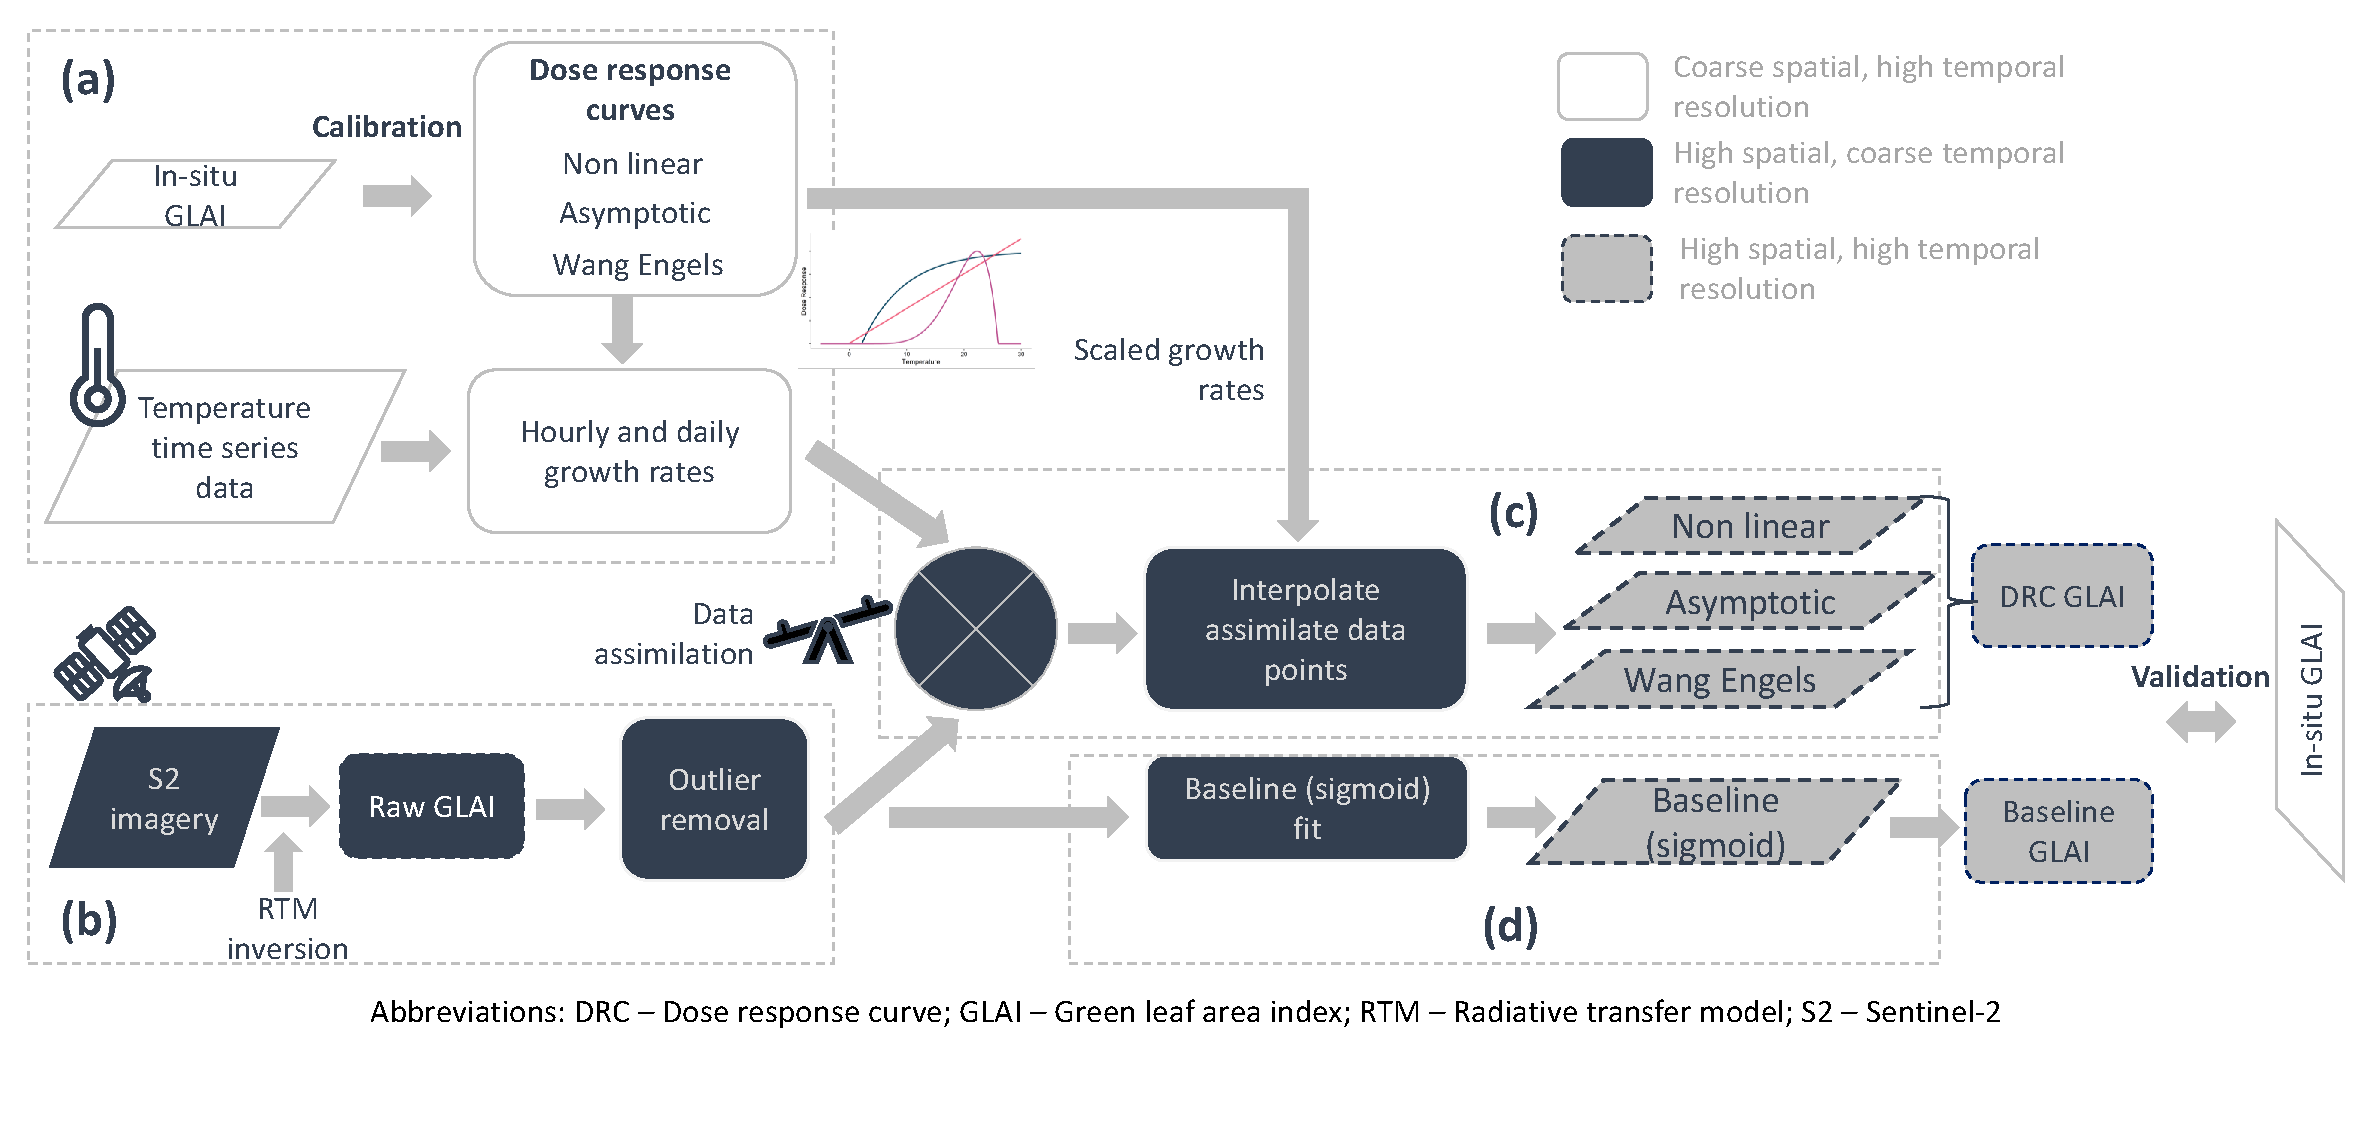
\includegraphics[width=1.0\textwidth]{06-DRC/img/workflow_glai_ts_reconstruction.pdf}
    \caption{Proposed workflow to reconstruct continuous \gls{GLAI} time series with high spatial and temporal resolution using temperature-based \gls{DRC}s to obtain \gls{GLAI} growth rates (a), \gls{S2} raw \gls{GLAI} observations per pixel (b) and data assimilation and \gls{DRC}-based interpolation of assimilated \gls{DRC} \gls{GLAI} values (c). The baseline method using a sigmoid function fit to the \gls{S2} \gls{GLAI} data (baseline \gls{GLAI}) is shown in (d).}
    \label{fig:workflow-glai-time-series}
\end{figure}

\subsection{Processing of in-situ data}
Throughout the main growing season of winter wheat (beginning of March till end of June in central Europe) continuous, mostly weekly measurements of \gls{GLAI} and phenology were undertaken at the calibration (Section~\ref{subsec:calibration-data}) and validation sites (Section~\ref{subsec:validation-data}). All measurements were linked to hourly air temperature readings 2 m above ground available from nearby weather stations.

\subsubsection{Air temperature data}
Air temperature data was acquired hourly 2 m above ground in deg C. In addition, the temperature readings were aggregated to daily resolution by averaging all 24 hourly measurements of a day from midnight to midnight.

\subsubsection{Green Leaf Area Index}
\label{subsubsec:glai-processing}
\gls{GLAI} samples were derived non-destructively using a LAI-2200C Plant Canopy Analyzer by LI-COR Biosciences with a 45 degree viewing cap. Measurements were performed at pre-defined sampling points within the fields (see, e.g., Figure~\ref{fig:map-validation-sites}a). For each measurement, three replicates were performed in different orientations each of them offset by 90 degrees. To avoid contamination of the measurement by direct sun light the measurements were either shaded manually, taken under diffuse light conditions (over-cast sky, fog) or acquired early in the morning.

\subsubsection{Phenology}
\label{subsubsec:phenology-processing}
Estimates of \gls{GLAI} (Section~\ref{subsubsec:glai-processing}) were linked to phenological development.
Phenological development of the winter wheat canopies was expressed in \gls{BBCH} scale following~\cite{lancashire_uniform_1991}. For the rating of the beginning of stem elongation (BBCH 30) we cut the main tiller lengthwise and measured the distance between the first node and the tillering node following the manual by~\cite{pask_physiological_2012}. End of heading (BBCH 59) was reached when the inflorescence was fully emerged.

\subsection{Model calibration to introduce physiological knowledge}
\label{subsec:model-cal}

Model calibration introduces the a-priori physiological knowledge about the relationship between plant growth and air temperature (Figure \ref{fig:workflow-glai-time-series}a). The knowledge was based on a dataset of in-situ \gls{GLAI} measurements from the calibration sites (Section~\ref{subsec:calibration-data}). The measured in-situ \gls{GLAI} values were used to calculate \gls{deltaGLAI} between two time points, which represent increase, respectively growth of the wheat canopy (Equation~\ref{eq:delta_LAI}) (as in \cite{tschurr_frost_2023}). In-situ \gls{GLAI} values have been smoothed using cubic smoothing splines before the calculation of \gls{deltaGLAI}.

\begin{equation}
\label{eq:delta_LAI}
  \Delta GLAI(t_n) =  GLAI(t_{n}) - GLAI(t_{n-1})\,,
\end{equation}

The \gls{deltaGLAI} value can then be expressed using the temperature trajectory between time point t\textsubscript{n} and t\textsubscript{n-1} in either hourly or daily granularity.

\subsubsection{Fitting of Dose-Response Curves}
\label{subsubsec:fitting-drc}
% DRCs
The calibration dataset was utilised to optimise three distinct \gls{DRC}, as illustrated in Figure~\ref{fig:DRC_overview}. Each curve represents the behaviour of the \gls{deltaGLAI} as a function of the observed temperature. The simplest \gls{DRC} displays a non-linear correlation between growth and temperature, with zero growth deemed below $T_{base}$. A linear growth reaction is projected for temperatures exceeding $T_{base}$. We hereafter refer to this growth response curve as the non-linear DRC (e.g., as seen in \cite{roth_field_2023}). Additionally, an asymptotically shaped DRC was employed, accounting for a base temperature ($T_{base}$), below which no growth occurs. Above $T_{base}$, the DRC exhibits a maximum growth response, defined by the curve's asymptote, along with the parameter lrc, allowing for an asymptotic shape of the curve (e.g., see \cite{roth_phenomics_2022}). Similar to the asymptotic \gls{DRC}, the Wang Engels \gls{DRC} can be defined by three parameters: $T_{base}$, which is the temperature below which growth does not occur, $T_{opt}$, which defines the highest growth rate response, and $T_{max}$, which is the temperature above which the growth rate is set to zero~\citep{wang_simulation_1998, wang_uncertainty_2017} (refer to Figure~\ref{fig:DRC_overview}).

\begin{figure}[H]
    \centering
    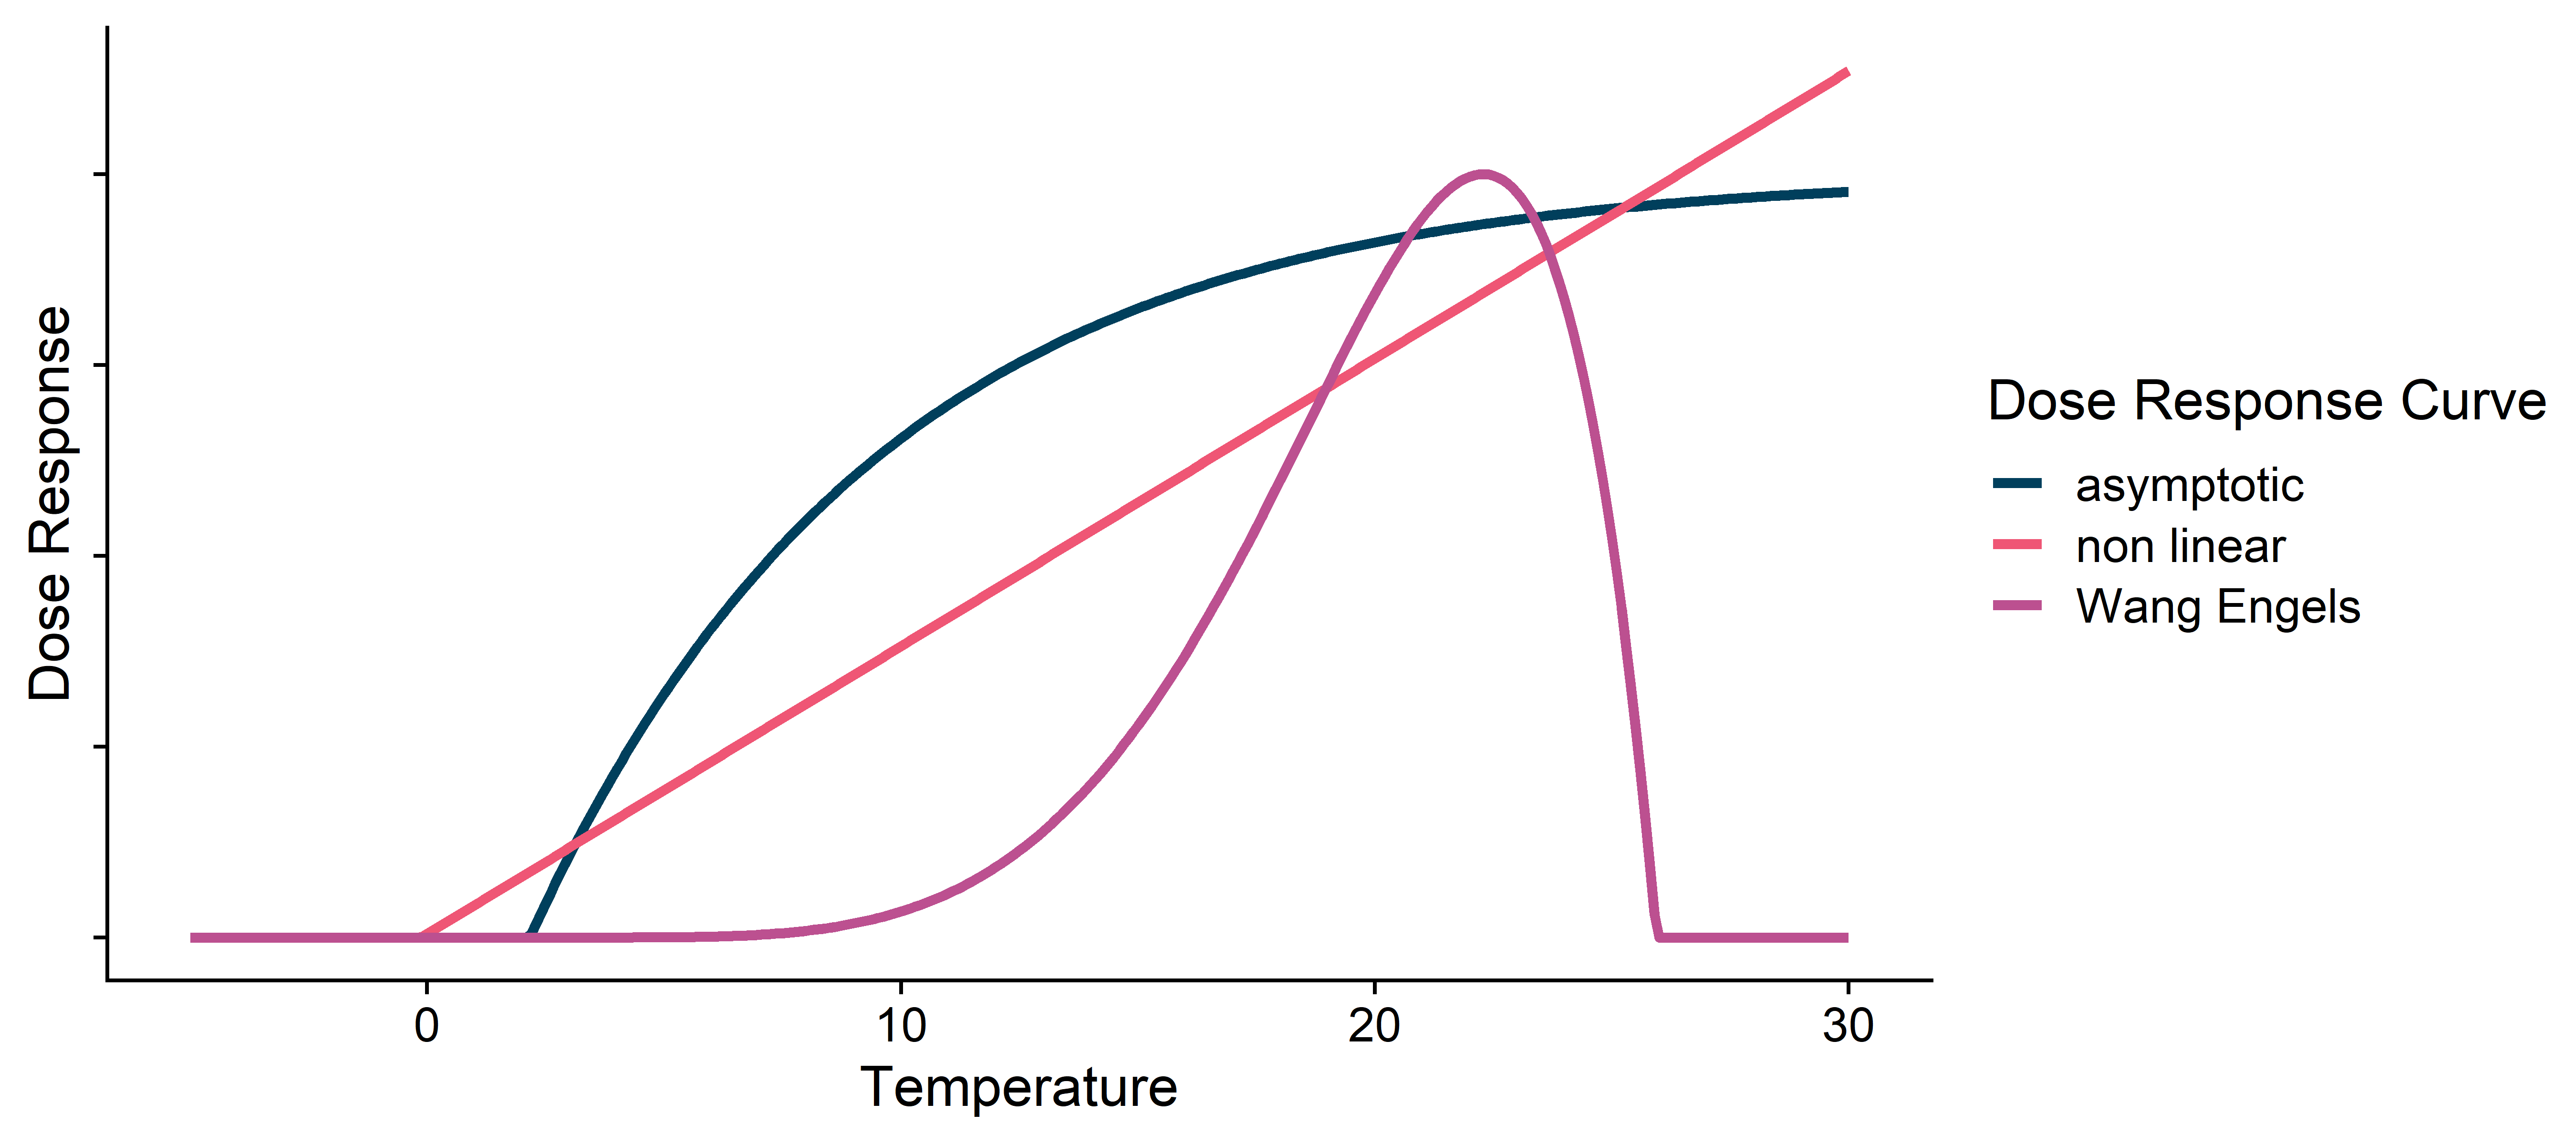
\includegraphics[width=0.8\textwidth]{06-DRC/img/DRC_curves_scheme.png}
    \caption{Schematic overview of the three used dose response curves (DRC), non linear, asymptotic and Wang Engels curve. The x axis represents the input temperature, the y axis the corresponding response in green leaf area index (GLAI) growth.}
    \label{fig:DRC_overview}
\end{figure}


\begin{table}[H]
\caption{Dose response curve parameters and constraints used for model fitting.}
\label{tab:drc_fitting}
\centering
\begin{tabular}{lll}
Dose response curve & parameters                       & constraints                          \\ \hline
non linear          & $T_{base}$ , slope         &                                      \\
asymptotic          & $T_{base}$, lrc, asymptote & $T_{base}$ \textless asymptote \\
Wang Engels &
  \begin{tabular}[c]{@{}l@{}} $T_{base}$,\\  $T_{opt}$,\\   $T_{max}$\end{tabular} &
  \begin{tabular}[c]{@{}l@{}} $T_{base}$\\  \textless $T_{opt}$ \\ \textless  $T_{max}$\end{tabular}
\end{tabular}
\end{table}

% fitting nloptr
The parameters for each of the three DRCs (refer to Table~\ref{tab:drc_fitting}) were optimised utilising the calibration data explained earlier. An augmented Lagrangian algorithm employing the nloptr package in R \citep{rcore-team_r_2014,johnson_nlopt_2007} was used for this purpose. Regarding our third research question, optimisation was conducted for temperature values of both hourly and daily measurements.

As the curves used can solely depict ascending \gls{GLAI} values, we excluded negative \gls{deltaGLAI} values prior to optimization. These values are typically attributable to measurement uncertainty and imprecisions, such as those related to sensor positioning. As a result, 20\% of \gls{deltaGLAI} values were rejected. Constrained optimization by linear approximation (COBYLA) was used as the local solver for optimization, providing upper and lower bounds and a starting value \citep{powell_direct_1994}. Initial values were determined either by quantile values of input temperature data (for $T_{base}$, $T_{opt}$, and $T_{max}$) or by empirically derived values (slope, lrc, and asymptote) (refer to Table \ref{tab:Sup_starting_paramters} in the Appendix). Optimisation was carried out 20 times on a randomly selected 80\% of the data, and the final parameters were derived from the median of the 20 subset optimisations to obtain more robust parameter values, thereby reducing the possible influence of outliers. For each temperature measurement, the corresponding dose response value was calculated and accumulated over time. To optimise the parameters, the \gls{RMSE} between these accumulated values and the \gls{deltaGLAI} measurements was minimised. The skill score was negatively impacted for meeting constraints (Table~\ref{tab:drc_fitting}) or for forecasting \gls{deltaGLAI} values that were too low to attain physiologically significant parameter and prediction values.

\subsection{Processing of \gls{S2} data}

\gls{S2} raw \gls{GLAI} observations introduce spatial detail (Figure \ref{fig:workflow-glai-time-series}b).
We used all 10 and 20 m bands except band 8 (central wavelength 842 nm). Band 8 was discarded in favor of band 8A (central wavelength 865 nm) which provides a higher spectral resolution than band 8. Thus, nine bands between 492 and 2200 nm were used: B2 (blue), B3 (green), B4 (red), B5 (red-edge 1), B6 (red-edge 2), B7 (red-edge 3), B8A (near-infrared 2), B11 (shortwave-infrared 1), and B12 (shortwave-infrared 2). See also Table \ref{tab:s2-bands} in the Appendix for details about the native spatial resolution, spectral band widths and central wavelengths of these bands.

First, we clipped the \gls{S2} data to the spatial extent of the field parcels at the validation sites (Figure~\ref{fig:map-validation-sites}a). Next, we resampled the six 20 m bands (see Table \ref{tab:s2-bands}) to a spatial resolution of 10 m using nearest neighbor interpolation.

All scenes were pre-processed by ESA using the payload data ground segment (PDGS) baselines 4.00 (2022 data) and 5.09 (2023 data) that compromise an improvement radiometric harmonization of S2A and S2B as well as geometric refinements that fulfil the CEOS Analysis Ready Data for Land (CEOS ARD) standard. Therefore, no further refinements such as image co-registration were undertaken.

\subsubsection{Data cleaning}
We used the \gls{SCL} delivered as part of the \gls{S2} L2A product to filter out clouds, shadows, open water, snow and cirrus on a per-pixel basis. Thus, only the SCL classes 4 (vegetation) and 5 (bare soil) were kept. Pixel values with a different \gls{SCL} class assignment were masked and not considered any further.

\subsubsection{Radiative transfer modelling}
To extract raw \gls{GLAI} from \gls{S2} scenes at the validation sites (Section~\ref{subsec:s2-imagery}) we used the four-stream \gls{RTM} PROSAIL~\citep{jacquemoud_prospectsail_2009} to simulate bi-directional reflectance factors of winter wheat canopies. PROSAIL couples the leaf \gls{RTM} PROSPECT-D~\citep{feret_prospect-d_2017} with the canopy \gls{RTM} 4SAIL~\citep{verhoef_light_1984}. We parameterized the \gls{RTM} inputs to reflect typical physiological and morphological characteristics of winter wheat canopies between \gls{BBCH} stages 30 and 59 based on a comprehensive field phenotyping dataset described in \cite{graf_insights_2023}. The leaf (PROSPECT-D) and canopy (4SAIL) input parameters including their range and distribution are shown in Table~\ref{tab:drc-prosail-inputs} based on \cite{graf_insights_2023}. Following the proposed workflow by \cite{graf_insights_2023} we increased the physiological plausibility of \gls{RTM} inputs. In detail, the leaf chlorophyll a+b and leaf carotenoid content were re-distributed based on empirical relationships between these traits and the \gls{GLAI} established in \cite{graf_insights_2023} (GLAI - Cab relationship) and \cite{wocher_rtm-based_2020} (Cab - Car relationship). Using these relationships we can re-distribute Cab (through the canopy chlorophyll content) solely based on \gls{GLAI}. Similarly, Car can be re-distributed solely based on Cab obtained in the previous step.

We run PROSAIL in forward mode based on the input parameters denoted in Table~\ref{tab:drc-prosail-inputs} for each \gls{S2} scene during the stem elongation period. Illumination and observer angles were set to scene-specific values obtained from the \gls{S2} scene metadata. In total, we run 50 000 PROSAIL simulations per \gls{S2} scene. The resulting spectra were converted to the spectral resolution of \gls{S2} by convolution of the original PROSAIL outputs in 1 nm spectral resolution with the spectral response functions of \gls{S2}A and B provided by ESA\footnote{\url{https://sentinel.esa.int/web/sentinel/user-guides/sentinel-2-msi/document-library/-/asset_publisher/Wk0TKajiISaR/content/sentinel-2a-spectral-responses}}. In addition, we applied further physiological plausibility checks introduced by~\cite{wocher_rtm-based_2020}. In detail, we dropped simulated spectra with a shift of the green reflectance peak towards wavelengths shorter than 574 nm, which was considered implausible based on extensive survey of handheld and airborne hyperspectral imaging data of green vegetation. Around 10\% of the simulated PROSAIL spectra were therefore discarded. The resulting spectra were stored in lookup tables (\gls{LUT}s) per \gls{S2} scene.

\begin{table}[H]
\caption{Parameter ranges and distributions for the combined leaf (PROSPECT-D) and canopy (4SAIL) \gls{RTM} (PROSAIL) for winter wheat canopies in the stem elongation phase. The ranges are given for uniform distributions (range) or a truncated Gaussian distribution with mean and standard deviation denoted in brackets. Cab and Car are redistributed on \gls{GLAI}. All values and distributions are taken from \cite{graf_insights_2023}.}
\label{tab:drc-prosail-inputs}
\begin{tabular}{@{}lllllll@{}}
\toprule
  \textbf{Trait}     & \textbf{Description}         & \textbf{Unit}           & \multicolumn{4}{l}{\textbf{Range}}              \\ \midrule
\multicolumn{7}{l}{\textbf{PROSPECT-D (Leaf)}}                                                                \\
\midrule
N      & Leaf Structure Parameter     & {[}-{]}                 & \multicolumn{4}{l}{1 - 2.5 (1.5, 0.2)}          \\
Cab    & Leaf Chlorophyll a+b Content & {[}$\mu g$ $cm^{-2}${]} & \multicolumn{4}{l}{redistributed based on GLAI} \\
Car    & Leaf Carotenoid Content      & {[}$\mu g$ $cm^{-2}${]} & \multicolumn{4}{l}{redistributed based on Cab}  \\
Cant   & Leaf Anthocyanin Content     & {[}$\mu g$ $cm^{-2}${]} & \multicolumn{4}{l}{0.0 - 5.0 (2.0, 0.8)}        \\
Cbrown & Brown Pigments               & {[}-{]}                 & \multicolumn{4}{l}{0 - 1}                       \\
Cw     & Equivalent Water Thickness   & {[}cm{]}                & \multicolumn{4}{l}{0 - 0.07 (0.04, 0.02)}       \\
Dm     & Dry Matter Content           & {[}$g$ $cm^{-2}${]}     & \multicolumn{4}{l}{0 - 0.01}                    \\
\midrule
\multicolumn{7}{l}{\textbf{4SAIL (Canopy)}}                                                                     \\
\midrule
GLAI   & Green Leaf Area Index        & {[}$m^2$ $m^{-2}${]}    & \multicolumn{4}{l}{0.5-6.5}                         \\
ALA    & Leaf Inclination Angle       & {[}deg{]}               & \multicolumn{4}{l}{30 - 70}                     \\
hspot  & Hot spot Parameter           & {[}-{]}                 & \multicolumn{4}{l}{0.01 - 0.5}                  \\
rsoil  & Soil Brightness Factor       & {[}-{]}                 & \multicolumn{4}{l}{0 - 1}                       \\
psoil  & Dry/ Wet Soil Factor         & {[}-{]}                 & \multicolumn{4}{l}{0 - 1}                       \\ \bottomrule
\end{tabular}
\end{table}


\subsubsection{Radiative transfer model inversion}
\label{subsubsec:rtm-inv}
For \gls{RTM} inversion we used the PROSAIL spectra stored in \gls{LUT}s per scene. We retrieved raw \gls{GLAI} per \gls{S2}  pixel by comparing \gls{S2}-observed ($\rho_{S2}$) spectra with the simulated spectra in the \gls{LUT} ($\rho_{LUT}$) by means of the \gls{MAE} for all $n$ \gls{S2}-bands considered (i.e., $n=9$) as suggested by \cite{graf_insights_2023}.

\begin{equation}
    MAE = \frac{1}{n} \sum_{i=0}^{n} |\rho_{{S2}_i} - \rho_{{LUT}_i} |
\end{equation}
The median \gls{GLAI} value obtained from the 5000 simulated spectra with the smallest \gls{MAE} was then used as the \gls{S2}-derived raw \gls{GLAI} observation per \gls{S2} pixel.


\subsection{Time series reconstruction}
\label{subsec:drc-model-inference}

\subsubsection{DRC-derived growth rates at the farm scale}

Fitted \gls{DRC}s were applied to hourly and daily air temperature data at the validation sites (Section~\ref{subsec:validation-data}, Figure \ref{fig:workflow-glai-time-series}a). This converted each air temperature reading into a \gls{GLAI} growth rate. Thus, per site and \gls{DRC} \gls{GLAI} growth rates in hourly and daily resolution were available.

\subsubsection{S2-derived raw GLAI observations at the pixel scale}
\label{subsubsec:s2-glai-simple-outlier-filter}
A simple outlier detection formalism was introduced to account for undetected atmospheric disturbances in the raw \gls{S2} \gls{GLAI} observations (Figure \ref{fig:workflow-glai-time-series}b). Atmospheric disturbances usually cause negatively biased outliers in remotely-sensed trait observations~\citep{chen_simple_2004}. Therefore, raw \gls{S2} \gls{GLAI} values of a pixel that deviated from the mean of all raw \gls{GLAI} values by more than a single standard deviation in the negative y-direction were discarded. This did not apply to the first \gls{GLAI} observation in time due to two reasons: First, we lack sufficient temporal context. Second, due to its proximity to the early phase of stem elongation a low \gls{GLAI} value is physiologically plausible.

\subsubsection{Data assimilation using Ensemble Kalman Filtering}
We aimed to combine the modelled \gls{DRC} \gls{GLAI} growth rates reflecting a-priori physiological knowledge about the relationship of growth to air temperature with raw \gls{S2} \gls{GLAI} observations to obtain the best possible estimate of the effective \gls{GLAI} (Figure \ref{fig:workflow-glai-time-series}c). Combining models with observations presents a data assimilation problem. In our case, we assimilated the raw \gls{S2} \gls{GLAI} observations into the \gls{DRC}-based \gls{GLAI} growth rates to introduce spatial detail while retaining the high temporal resolution and physiological meaning of the underlying temperature data.

For data assimilation, the \gls{KF} is widely used. In essence, \gls{KF} is a sequential approach estimating the "true", hidden state vector of a system by updating the modelled states whenever an observation becomes available. In our case, the hidden state vector is given by the actual but unknown \gls{GLAI} time series of a pixel. Since, both, the \gls{DRC} models and the \gls{S2} observations have uncertainties, we use the probabilistic \gls{EnsKF}. The \gls{EnsKF} allows to include model and observation uncertainty into the data assimilation process~\citep{evensen_ensemble_2003}. \gls{EnsKF} frameworks have therefore been widely used in assimilating remotely sensed crop traits in crop models~\citep{de_wit_crop_2007, zhao_assimilating_2013, huang_assimilating_2016}. ~\cite{graf_propagating_2023} found that raw \gls{GLAI} values derived from \gls{S2} take relative standard uncertainties up to 5\% due to uncertainty in the \gls{S2} top-of-atmosphere reflectance data. For in-situ \gls{GLAI} and temperature data we estimated a similar magnitude of uncertainty and set relative model uncertainty to 5\%. The \gls{EnsKF} ensemble size was set to 50 ensemble members to balance computational complexity with statistical significance as suggest by ~\cite{de_wit_crop_2007} and ~\cite{zhao_assimilating_2013}.

Figure~\ref{fig:assimilation-sample-pixel} shows the proposed data assimilation approach, i.e., a zoom-in into Figure~\ref{fig:assimilation-sample-pixel}c, for a randomly selected \gls{S2} pixel at the Strickhof site in 2022. Figure \ref{fig:assimilation-sample-pixel}a denotes the hourly air temperature time series available from the nearby weather station that was input into the \gls{DRC}s to obtain hourly \gls{GLAI} growth rates. The raw \gls{S2} \gls{GLAI} observations (red dots) were assimilated into the \gls{DRC} \gls{GLAI} growth rates (Figure \ref{fig:assimilation-sample-pixel}b) and subsequently used to reconstruct the final \gls{DRC} \gls{GLAI} time series with uncertainties (Figure \ref{fig:assimilation-sample-pixel}c). Below we explain the steps in more detail.

\begin{figure}[H]
    \centering
    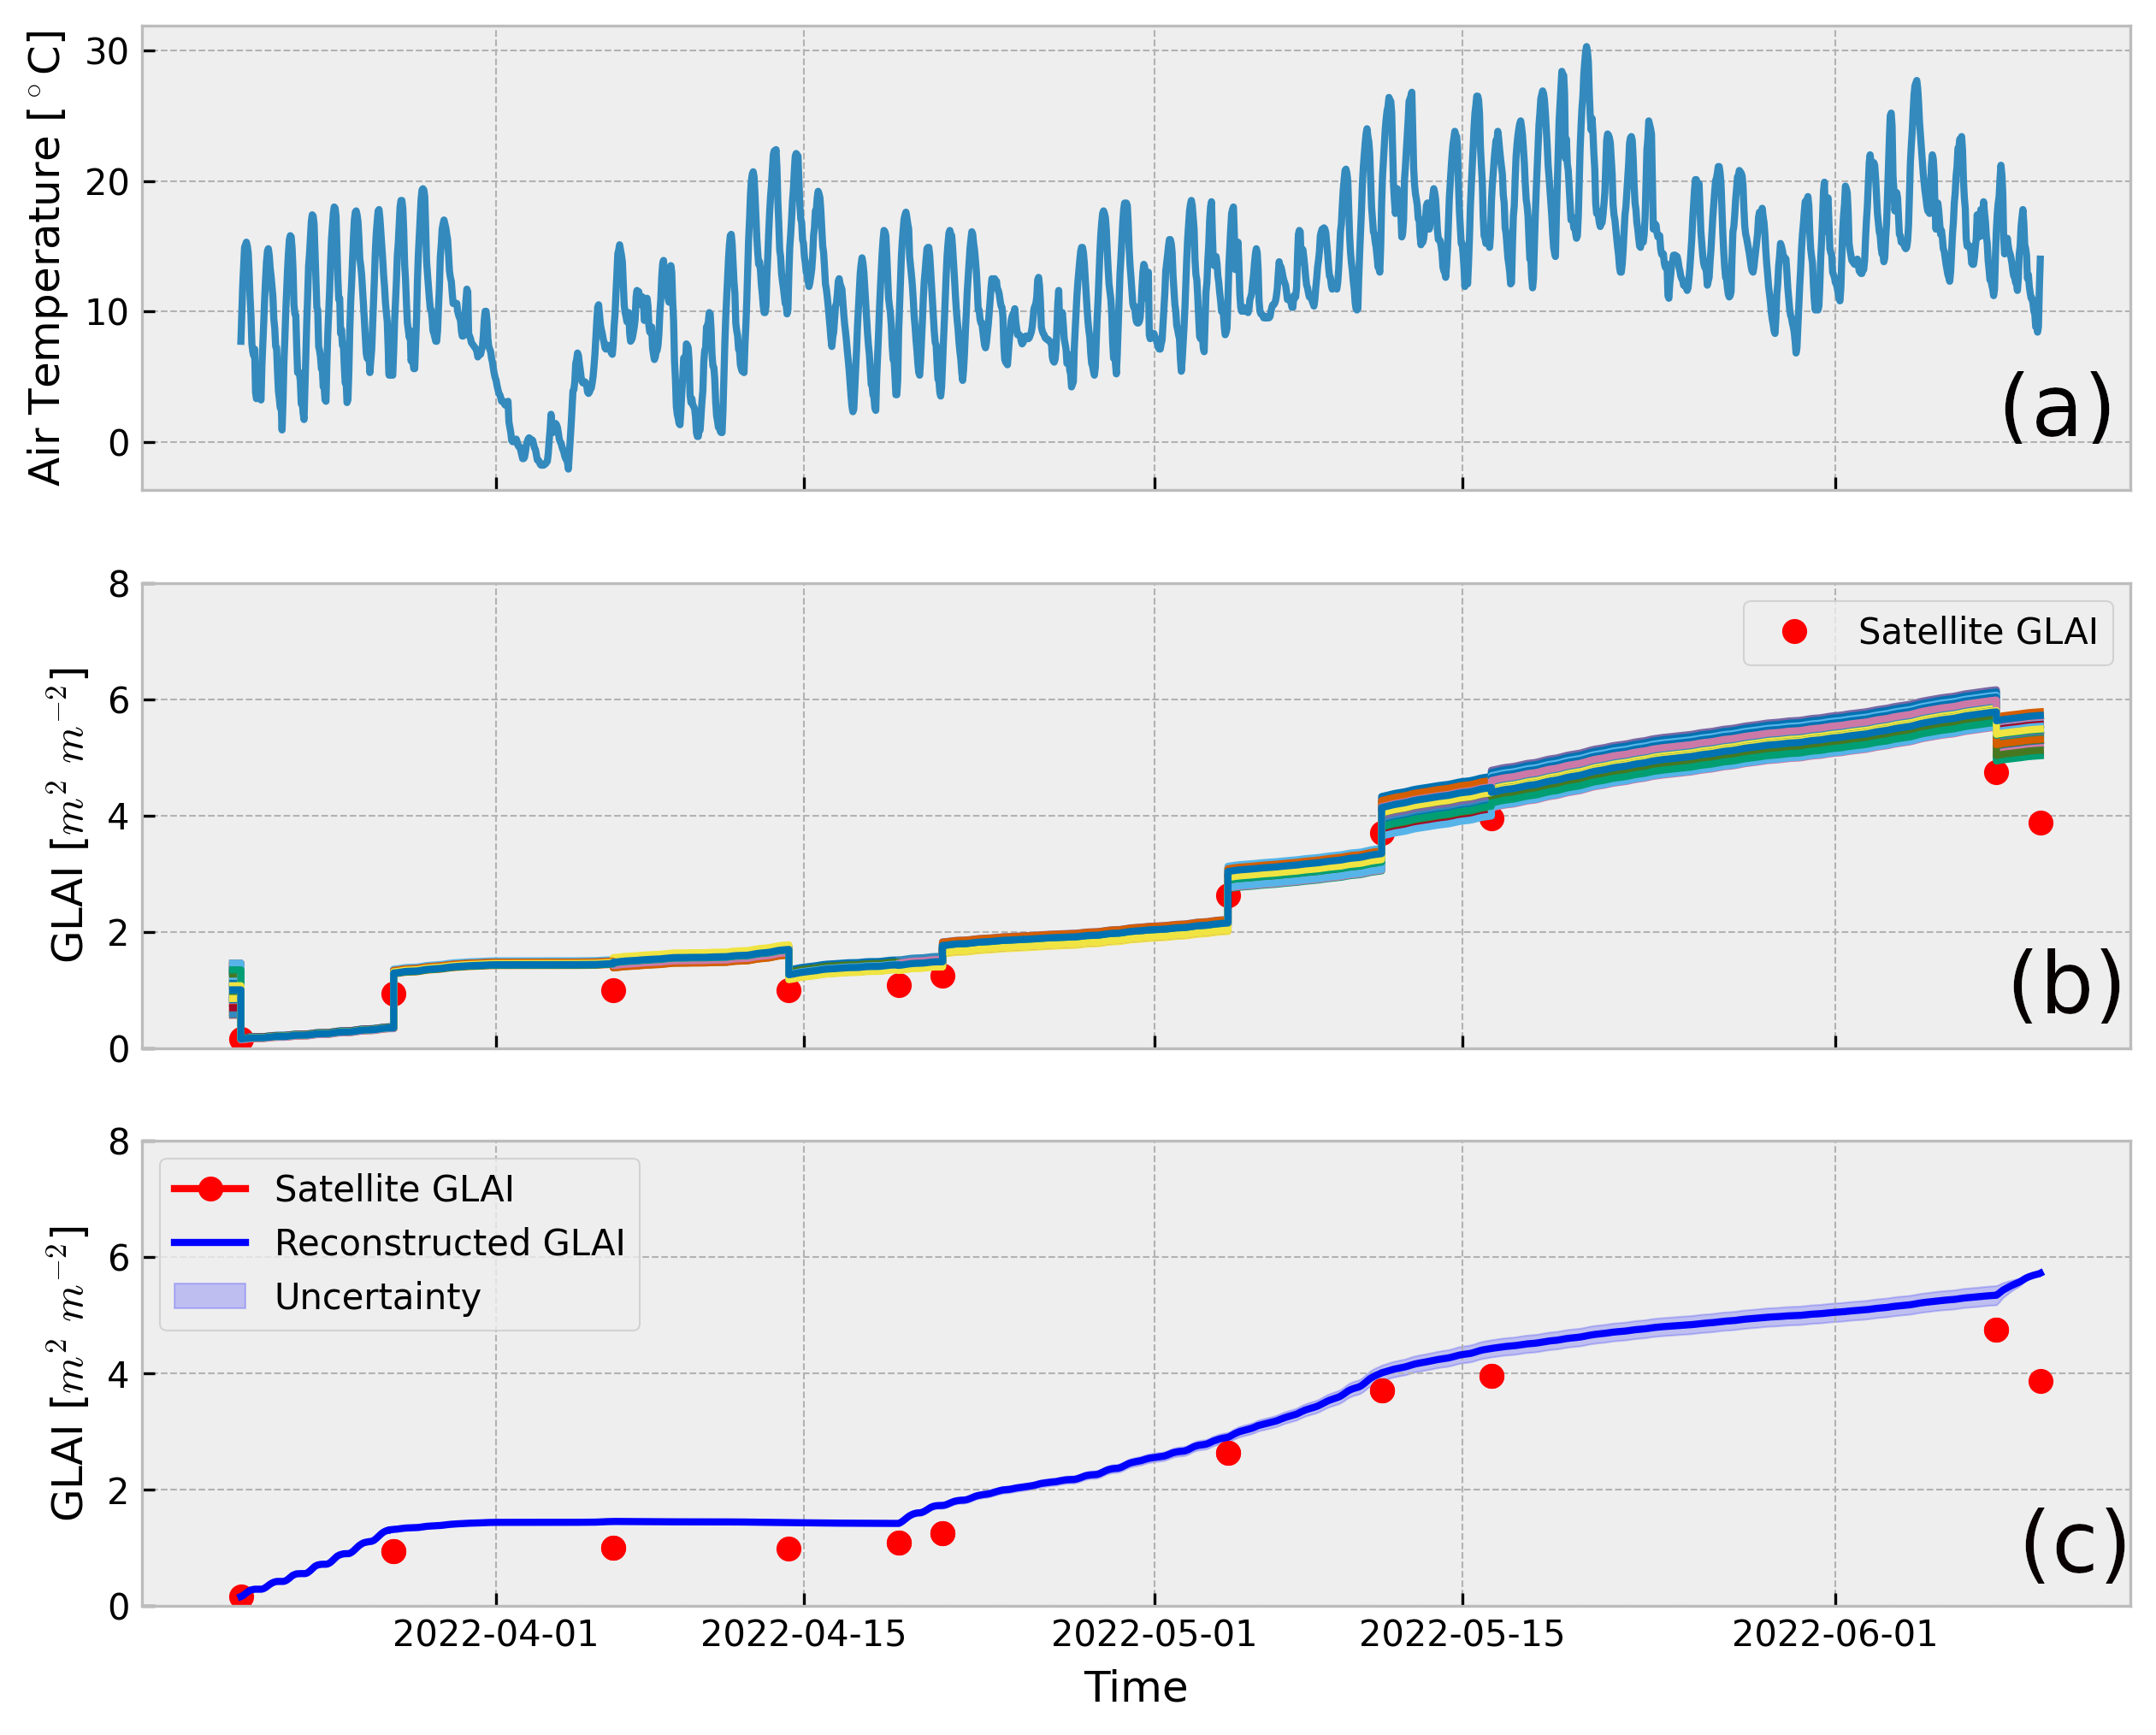
\includegraphics[width=\textwidth]{06-DRC/img/interpolated_lai_5255495.0_475965.0_hourly.png}
    \caption{Example of the proposed probabilistic \gls{GLAI} assimilation for a single \gls{S2} pixel at the Strickhof site in 2022 combining hourly air temperature data (a) with raw \gls{S2} \gls{GLAI} observations (red dots) using \gls{DRC}-based cumulative daily growth rates (solid colored lines in b) to reconstruct \gls{GLAI} time series with associated uncertainties (c). The dose-response curve type used in this case was asymptotic.}
    \label{fig:assimilation-sample-pixel}
\end{figure}

As a first step, we performed a conventional \gls{EnsKF} assimilation (Figure~\ref{fig:assimilation-sample-pixel}b) using \gls{DRC}-based growth rates derived from air temperature time series (Figure~\ref{fig:assimilation-sample-pixel}a). As the \gls{DRC}s provide growth rates, an initial \gls{GLAI} must be provided. We therefore initialised each of the 50 ensembles by randomly sampling between the lower and upper \gls{GLAI} bounds using a uniform probability distribution. The initial \gls{GLAI} bounds were set to a range of 0.5 to 1.5$m^2$ $m^{-2}$ based on empirical knowledge. We started the model runs just before the first \gls{S2} observation (Figure~\ref{fig:assimilation-sample-pixel}b, left). We then accumulated all the \gls{DRC} \gls{GLAI} growth rates up to the first raw \gls{S2} \gls{GLAI} observation. At the time $t$ of the observation, we computed the Kalman gain $K$:

\begin{equation}
\label{eq:kalman-gain}
    K = P_e H^T (H P_e H^T + R_e)^{-1}
\end{equation}
In Equation~\ref{eq:kalman-gain}, $P_e$ and $R_e$ denote the model and observation covariance matrices based on their uncertainties, and $H$ is the measurement operator which is the identity matrix since \gls{GLAI} is directly observable. Using $K$, we calculate the Kalman innovation term $KI$

\begin{equation}
    KI = D - (H A)
\end{equation}
where $D$ denotes the observation matrix with uncertainties and $A$ is the matrix with modelled \gls{GLAI} values at time $t$. Thus, the model state at the analyses step $A^a$ can be obtained:

\begin{equation}
\label{eq:kalman-analyses-step}
    A^a = A + K\ KI
\end{equation}
$A^a$ re-initializes the ensembles at $t$. As before, we then calculated the cumulative \gls{DRC} growth rates until the next raw \gls{S2} \gls{GLAI} observation at time $t+1$. At $t+1$ a new $A^a$ was calculated using Equations~\ref{eq:kalman-gain} to~\ref{eq:kalman-analyses-step}. This procedure was repeated for all \gls{S2} observations except the last one as shown in Figure~\ref{fig:assimilation-sample-pixel}b.

Here, a limitation of the \gls{EnsKF} method becomes clear: \gls{EnsKF} is a non-conservative approach, i.e., potentially large jumps in the modeled time series are caused by the assimilation (Figure~\ref{fig:assimilation-sample-pixel}b). This is physiologically implausible, since GLAI trajectories must be continuous. Therefore, we had to extended the EnsKF approach in a second step:

We addressed said problem by replacing the raw \gls{S2} \gls{GLAI} observations with the ensemble mean at each analysis step $A^a$ ($GLAI_{assim}$). This is to ensure that model and observation information is preserved. The ensemble standard deviation is retained as a measure of uncertainty, taking into account both, model and observation uncertainty. Using the $GLAI_{assim}$ values, we used the \gls{DRC}s for a second time to model growth. This time, however, we used the \gls{DRC}s to interpolate between the $GLAI_{assim}$ values, which are still temporally sparse. We scaled the cumulative growth rates to exactly match the $GLAI_{assim}$ values. In case $GLAI_{{assim}_{t+1}}$ was smaller than $GLAI_{{assim}_{t}}$, $GLAI_{{assim}_{t+1}}$ was discarded. In this case, we interpolated between $GLAI_{{assim}_t}$ and $GLAI_{{assim}_{t+2}}$. This ensured that undetected outliers in the raw \gls{S2} \gls{GLAI} values were not given too much weight, while preserving medium range temporal characteristics. The resulting interpolated \gls{GLAI} curve at the temporal resolution of the \gls{DRC} (i.e., hourly or daily) is shown in Figure~\ref{fig:assimilation-sample-pixel}c, in which the solid blue line denotes the assimilated, \gls{DRC}-interpolated reconstructed \gls{GLAI} time series.

From here on we name the reconstructed time series after the underlying \gls{DRC}s. That is, by "non linear" we mean from now on the \gls{EnsKF} assimilated and interpolated data points created using the non linear \gls{DRC} and raw \gls{S2} \gls{GLAI} observations. The same applies to "asymptotic" and "Wang Engels".

\subsubsection{Baseline method}
\label{subsubsec:baseline-method}
As baseline method, a sigmoid (a.k.a. logistic) function was fitted to the same raw \gls{S2} \gls{GLAI} observations at the pixel scale (Figure~\ref{fig:workflow-glai-time-series}d). Due to its S-shaped form, sigmoid functions are widely used in remote sensing to obtain continuous time series of vegetation traits. The sigmoid function is a simplified version of \gls{DL}~\citep{beck_improved_2006}, which only accounts for the generative (ascending) branch of \gls{GLAI} development. It is therefore a baseline that, unlike other statistical models such as the Savitzky-Golay filter, already has parameters with a certain biological significance.

The sigmoid function takes four parameters: The supremum of the function's values $L$, the growth rate $k$, the function's midpoint $x_0$ and an offset from zero $b$ which is necessary because \gls{GLAI} values around \gls{BBCH} 30 are usually larger than zero:

\begin{equation}
\label{eq:logistic-function}
    f(x) = \frac{L}{1 + e^{-k(x-x_0)}} + b
\end{equation}

A minimum of four raw \gls{S2} \gls{GLAI} observations are required to fit the model parameters. We fit the sigmoid function to each pixel, taking into account all available \gls{GLAI} observations, using the Levenberg-Marquardt algorithm available in the scipy Python library (version 1.11.0) with the function "scipy.optimze.curve\_fit". The maximum number of optimisation steps was set to 1000. The parameterised logistic function (equation~\ref{eq:logistic-function}) was then used to reconstruct the \gls{GLAI} time series at daily resolution. We will refer to this time series as the baseline \gls{GLAI}.

\subsection{Model Validation}

The raw \gls{S2} \gls{GLAI} observations and the reconstructed continuous \gls{DRC} and baseline \gls{GLAI} time series were compared against the independent in-situ validation \gls{GLAI} data (Section~\ref{subsec:validation-data}). We obtained matching tuples of reconstructed and in-situ \gls{GLAI} by time stamp and spatial intersection of the sampling points with the \gls{S2} 10 m pixel grid. In the case of the reconstructed time series (i.e., \gls{DRC} and baseline \gls{GLAI}), each in-situ \gls{GLAI} value could be matched to a modelled \gls{GLAI} value as the time series is continuous and spans the whole time period for which in-situ data was available. For the raw \gls{S2} \gls{GLAI} observations this was not the case due to the aforementioned temporal sparsity of the satellite observations. Therefore, we only used in-situ \gls{GLAI} values that had a satellite overpass with a maximum difference of one day.

Comparison was carried out by means of common error measures of the linear regression between modelled and observed values. Error measures included the \gls{RMSE}, \gls{nRMSE}, \gls{R2}, and bias between reconstructed ($GLAI_{reconstructed}$) and in-situ \gls{GLAI} values ($GLAI_{insitu}$). The bias was calculated using the variance of $GLAI_{reconstructed}$ ($var(GLAI_{reconstructed})$) and the mean of the squared differences ($MSD$) between mean $GLAI_{reconstructed}$, $\mu(GLAI_{reconstructed})$, and $GLAI_{insitu}$ considering all $n$ matching tuples available:

\begin{equation}
    MSD = \frac{1}{n} \sum_{i=0}^{n} (\mu(GLAI_{reconstructed}) - GLAI_{{insitu}_i})^2
\end{equation}
\begin{equation}
    Bias = MSD - var(GLAI_{reconstructed})
\end{equation}

Error statistics were produced for all sites and years as well as for single sites, years and \gls{BBCH} macro stages (i.e, \gls{BBCH} 30-39, 50-59) to assess model performance in space, time, and with respect to phenological development. In addition, we visualized the temporal trajectories of \gls{GLAI} per parcel to evaluate the physiological plausibility and consistency of the reconstructed \gls{GLAI} time series.

We start with describing how the S2 imagery (Section \ref{subsec:process-s2}) was pre-processed, phenology (Section \ref{subsubsec:phenology-recoding}) and functional trait data (Section \ref{subsubsec:trait-measurement}) were measured in-situ, and how the meteorological data were converted to thermal time (Section \ref{subsubsec:meteo-data-processing}). Next, we describe the workflow from i) model calibration using field phenotyping data (Section \ref{subsec:model-calibration}) to ii) model inference on S2 imagery (Section \ref{subsec:model-inference}) to iii) model validation using data from on-farm trials (Section \ref{subsec:model-validation}). The source code to reproduce the entire workflow is openly available under GNU General Public License v3.0 (see \nameref{sec:code-data-availability}).

\subsection{Processing of S2 imagery}
\label{subsec:process-s2}
We resampled the 20 m S2 bands to 10 m spatial resolution. All 10 and 20 m bands were used except band 8 (832 nm central wavelength) resulting in a total of 9 bands considered. Band 8 was disregarded in favor of band 8A which has a higher spectral resolution and showed more accurate results in prior testing. In a next step, we clipped the S2 scenes to the extent of the field parcels using the open-source Python Earth Observation Data Analysis Library (EOdal, ~\citet{graf_eodal_2022}). We used the scene classification layer (SCL) of the Sen2Cor output to filter out all pixels except those classified as vegetated (SCL class 4) or bare soil (SCL class 5) to avoid contamination by clouds, shadows and snow.

\subsection{In-Situ data processing}
\label{subsec:in-situ-data-processing}

\subsubsection{Recording of phenology}
\label{subsubsec:phenology-recoding}
All measurements of GLAI and CCC at the field phenotyping (Section \ref{subsec:phenotyping-data}) and on-farm trial sites (Section \ref{subsec:on-farm-trials}) were linked to phenological stages. Phenological stages were expressed using the Biologische Bundesanstalt, Bundessortenamt and CHemical Industry (BBCH) scale. At all sites the rating of BBCH stages followed the work by~\citet{lancashire_uniform_1991}. Here, the rating of the transition between the three phenological macro stages considered deserves further detail, i.e., the beginning of SE (BBCH stage 31) and EH (BBCH stage 59).

SE (BBCH 31) was determined by cutting the main tiller lengthwise and measuring the distance between the first node and the tillering node following the manual by~\cite{pask_physiological_2012}. If the distance was >= 1 cm, the stage was recorded as BBCH 31. EH (BBCH 59) was determined as the stage when the inflorescence was fully emerged. The beginning of flowering (BBCH 61) was recorded when the first anthers became visible.

\subsubsection{Measurement of functional traits}
\label{subsubsec:trait-measurement}

\paragraph{Green Leaf Area Index}
GLAI was measured using destructive sampling at early growth stages and non-destructively after the onset of stem elongation (BBCH $>$33). For destructive sampling, the total surface biomass of a previously defined ground surface was sampled, with plants from at least two seed rows. From five to six randomly selected wheat plants in this sample, we took the top complete developed leaf (including leaf base) and placed them on a screen with known reference area. We determined the leaf area of these leaves $A_{leaf}$ by image segmentation, i.e., separated the leaves from the screen background. Subsequently, the total biomass as well as the leaves used for segmentation were freeze-dried for at least 48 hours and their dry weight was determined ($m_{total}$ and $m_{leaf}$, respectively). Using $m_{total}$ and $m_{leaf}$, we computed the total leaf area and, using the known ground area $A_{ground}$, the GLAI (Equation \ref{eq:destructive-glai}).

\begin{equation}
    \label{eq:destructive-glai}
    GLAI = \frac{A_{leaf} * \frac{m_{total}}{m_{leaf}}}{A_{ground}}
\end{equation}

From BBCH stage 33 onwards, this approach was no longer feasible as the increasing length of the leaves exceeded the reference grid. We therefore used a LAI-2200C Plant Canopy Analyzer by LI-COR Biosciences with a 45 degree viewing cap, performing replicates in three different orientations, each offset by 90 degrees. To avoid contamination of the measurement by direct sunlight, the measurements were mostly performed in the morning hours or under diffuse (cloudy) light conditions. A comparison of destructive and non-destructive methods was performed for individual data points and showed good agreement. GLAI measurements were continued until the onset of senescence in the lower leaf layers. Only at the SEON (Section \ref{subsubsec:seon-data}) and MNI (Section \ref{subsubsec:mni-data}) sites GLAI rating were continued after the onset of senescence estimating the fraction of non-photosynthetic leaf area by eye.

\paragraph{Canopy Chlorophyll Content}
CCC was estimated by destructively determining leaf chlorophyll content and GLAI. In 2019, the biomass samples were collected at experimental plots of the nitrogen fertilization experiments by~\cite{argento_investigating_2022} (see Section \ref{subsec:on-farm-trials}). For each plot, leaves were randomly selected. In 2022, the entire above ground biomass of two up to four seed rows at the sampling points was collected at a pre-defined distance. A randomly selected sub-sample was used for chlorophyll analysis. In both years, immediately after sampling, the leaves were frozen. In addition, the area of these leaves was determined in the same way as for GLAI to determine leaf mass per unit area. To avoid light damage, samples were stored in the dark. The frozen samples were weighed in a cooled container and freeze dried. After freeze drying, the samples were milled and prepared for the extraction. For this process, 50 $mg$ of the milled sample were mixed with ethanol (95\%, Analytical Grade) and the supernatant was removed from the sample for the analysis. This step was repeated two times or until the remaining pellet was of white-yellowish colour. In order to determine the pigment concentration in the supernatant, the absorbance of the supernatant was measured at 470 nm ($A_{470}$), 649 nm ($A_{649}$) and 664 nm ($A_{664}$) with a Microtitre plate reader (Infinite® M1000, Tecan) using a sample volume of 200 $\mu l$ with two replicates. From the absorbance the chlorophyll a ($c_a$) and b ($c_b$) and a+b ($c_{ab}$) content in $\mu g$ $ml^{-1}$ was calculated using the formula provided by~\citet{lichtenthaler_chlorophylls_2001}:

\begin{equation}
    c_a = 13.36 A_{664} - 5.19 A_{649}
\end{equation}

\begin{equation}
    c_b = 27.43 A_{649} - 8.12 A_{664}
\end{equation}

\begin{equation}
    c_{ab} = \frac{1000 A_{470} - 2.13 c_a - 97.64 c_b}{209}
    \label{eq:cab-tecan}
\end{equation}

The chlorophyll concentration obtained from Equation \ref{eq:cab-tecan} was related to leaf area using the known probe volume (200 $\mu l$ ethanol) and weight of the sample biomass (50 $mg$) dissolved in it. Using the LMA of the leaves the sample biomass was taken from we could then calculate the leaf chlorophyll content per area in $\mu g$ $cm^{-2}$ and scale it up to CCC using Equation \ref{eq:ccc-calc-rtm}. The required GLAI values were obtained from Equation \ref{eq:destructive-glai} based on the larger biomass samples or LI-COR measurements that were acquired in parallel to the leaf samples.

\subsubsection{Meteorological data processing}
\label{subsubsec:meteo-data-processing}

We used the daily mean air temperature 2 m above ground ($T_{abs}d$) from weather stations to calculate growing degree days (GDD, ~\cite{mcmaster_growing_1997}) for winter wheat assuming a base temperature ($T_{base}$) of zero degrees Celsius (Equation \ref{eq:GDD}). We obtained accumulative GDD (AGDD) by accumulating all GDDs obtained from Eq. \ref{eq:GDD} between the sowing and harvest date as reported by field calendars at the phenotyping (Table \ref{tab:phenotyping-datasources}) and on-farm sites (Figure \ref{fig:overview-map}).

\begin{equation}
\label{eq:GDD}
    GDD =
    \begin{cases}
        T_{abs}d & \text{if } T_{abs}d > T_{base} \\
        0 &  T_{abs}d \le T_{base}
    \end{cases}
\end{equation}

\subsection{Model Calibration}
\label{subsec:model-calibration}
For establishing physiologically plausible RTM inputs at the leaf and canopy level we consider correlations between leaf and canopy parameters (Section \ref{subsubsec:physiological-constraints}) and the dependency of GLAI to phenology and the dependency of phenology on air temperature (Section \ref{subsubsec:phenological-constraints}). All these insights are obtained from field phenotyping described in Section \ref{subsec:phenotyping-data} using the pre-processing methods explained in Section \ref{subsec:in-situ-data-processing}.

\subsubsection{Physiological Priors}
\label{subsubsec:physiological-constraints}

CCC and GLAI are closely correlated ~\citep{gitelson_remote_2005,gitelson_relationships_2014,gitelson_uncertainty_2022}. Following the approach proposed by ~\cite{wocher_rtm-based_2020} to account for the correlation between carotenoid (Car) and Cab content we established a relationship between CCC and GLAI to increase the physiological plausibility of RTM inputs using phenotyping data from the SEON and MNI sites (see Table \ref{tab:phenotyping-datasources} and Sections \ref{subsubsec:seon-data} and \ref{subsubsec:mni-data}).

Figure \ref{fig:lai-ccc-relationship} shows a strong linear relationship between CCC and GLAI obtained from field phenotyping with Pearson's $R^2$ 0.94 (N=137). We fitted a linear regression line to the data points and constructed an upper and lower envelope encompassing all data points. The linear regression with obtained coefficients is given in Equation \ref{eq:lin-regress}.

% linear regression formula
\begin{equation}
\label{eq:lin-regress}
    CCC = 0.5755 GLAI  % + 3.6287e^{-29}
\end{equation}

To fit the upper envelope, we used all CCC-GLAI pairs recorded before flowering (BBCH 61). Thus, we accounted for plant development during the vegetative (till BBCH 29) and reproductive phase in which CCC and GLAI are increasing steadily. A linear model was constructed and is denoted in Equation \ref{eq:upper-envelop}.

% upper envelop formula
\begin{equation}
\label{eq:upper-envelop}
    CCC_{upper} = 0.8544 GLAI % + 3.4852e^{-16}
\end{equation}

For the lower envelope we used all CCC-GLAI pairs recorded after BBCH 61. Here, we assume CCC and GLAI to decline with onset of senescence. We used a second order polynomial to construct the envelope (Equation \ref{eq:lower-envelop}). The reason for choosing a linear and polynomial model for the upper and lower envelope, respectively, follows the reasoning by~\cite{gitelson_relationships_2014}: During vegetative growth stages, the relationship between GLAI and CCC is strongly linear but tends to become polynomial for reproductive stages after flowering due to hysteresis effects.

\begin{equation}
\label{eq:lower-envelop}
    CCC_{lower} = 0.0763 * \left(\frac{GLAI}{1.6819}\right)^2 + 0.3336 * \frac{GLAI}{1.6819} - 0.0551
\end{equation}

\begin{figure}[H]
    \centering
    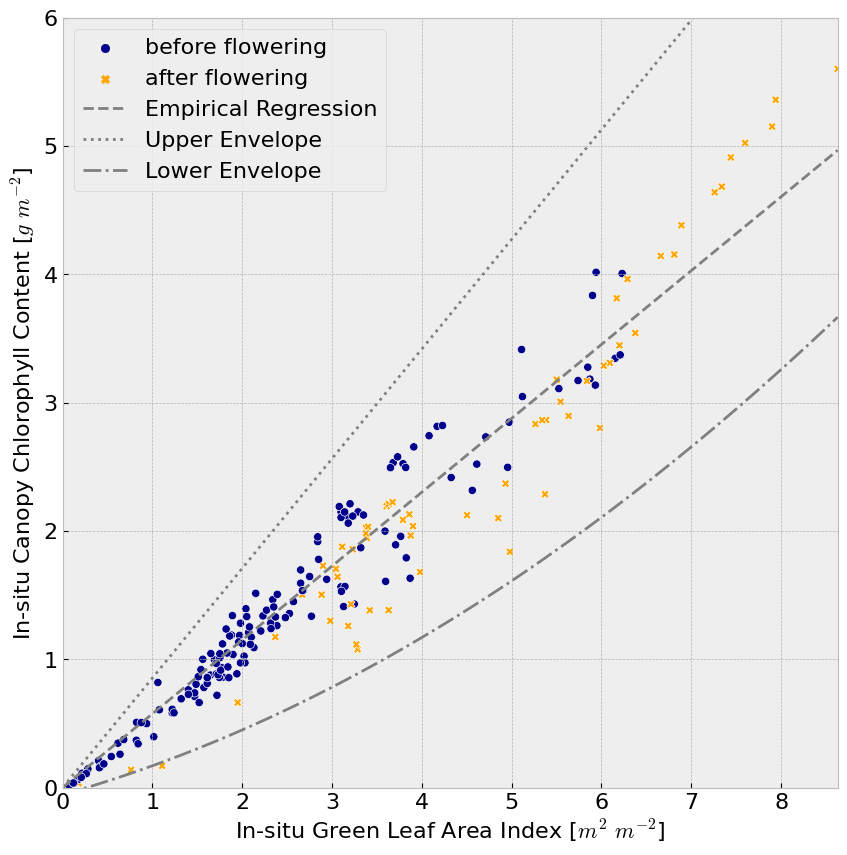
\includegraphics[width=1.0\textwidth]{empirical_relationship_gcc-glai.png}
    \caption[Empirical relationship between CCC and GLAI (N=137) obtained from field phenotyping data. The upper and lower envelope of the data are plotted fit for the data points recorded before and after flowering, respectively.]{Empirical relationship between CCC and GLAI (N=137) obtained from field phenotyping data. The upper and lower envelope of the data are plotted fit for the data points recorded before and after flowering, respectively.}
    \label{fig:lai-ccc-relationship}
\end{figure}

Following the approach by ~\cite{wocher_rtm-based_2020} we used the regression line and the envelopes to distribute CCC values using a truncated Laplacian distribution based on GLAI. Figure \ref{fig:constraints-in-lut} illustrates the principle: The left column in Figure \ref{fig:constraints-in-lut} (a, c, e) shows the relationship between CCC and GLAI (a), Cab and GLAI (c), and Car and Cab (e), when no physiological priors are included and the traits are, thus, uncorrelated. Here, a truncated normal distribution is assumed for Cab ($\mathscr{N} (50,40)$ $\mu g$ $cm^{-2}$) with a minimum of 0 and maximum of 80 $\mu g$ $cm^{-2}$ as suggested by~\cite{danner_efficient_2021}. Based on the same reference we obtained the uncorrelated Car samples (Figure \ref{fig:constraints-in-lut}e) with a minimum of 0 and maximum of 15 $\mu g$ $cm^{-2}$ using ($\mathscr{N} (7.5,5)$ $\mu g$ $cm^{-2}$). Our proposed workflow starts at Figure \ref{fig:constraints-in-lut}a with the redistribution of the CCC values based on the empirical relationship from Figure \ref{fig:lai-ccc-relationship} using Equations \ref{eq:lin-regress} to \ref{eq:lower-envelop}. The result is shown in Figure \ref{fig:constraints-in-lut}b: Low CCC values do not occur when GLAI values are high, which is consistent with the literature~\citep{gitelson_relationships_2014}. Using the redistributed CCC from Figure \ref{fig:constraints-in-lut}b, we redistributed Cab, using:

\begin{equation}
\label{eq:ccc-calc-rtm}
    CCC\ (g\ cm^{-2}) = Cab * GLAI * 0.01
\end{equation}
which can be rewritten to
\begin{equation}
\label{eq:ccc-calc-rtm_inv}
    Cab\ (\mu g\ cm^{2}) = \frac{CCC}{GLAI} * 100
\end{equation}
to calculate Cab from CCC and GLAI. The result is shown in Figure \ref{fig:constraints-in-lut}d: Low Cab values are removed when GLAI is high. In a last step, we used the redistributed Cab to implement the Car-Cab relation described in ~\cite{wocher_rtm-based_2020}. The result is depicted in Figure \ref{fig:constraints-in-lut}f. Thus, based on GLAI, CCC, Cab and Car are redistributed and mutually correlated based on empirical relationships from field phenotyping to establish physiologically plausible RTM inputs.

\begin{figure}[H]
    \centering
    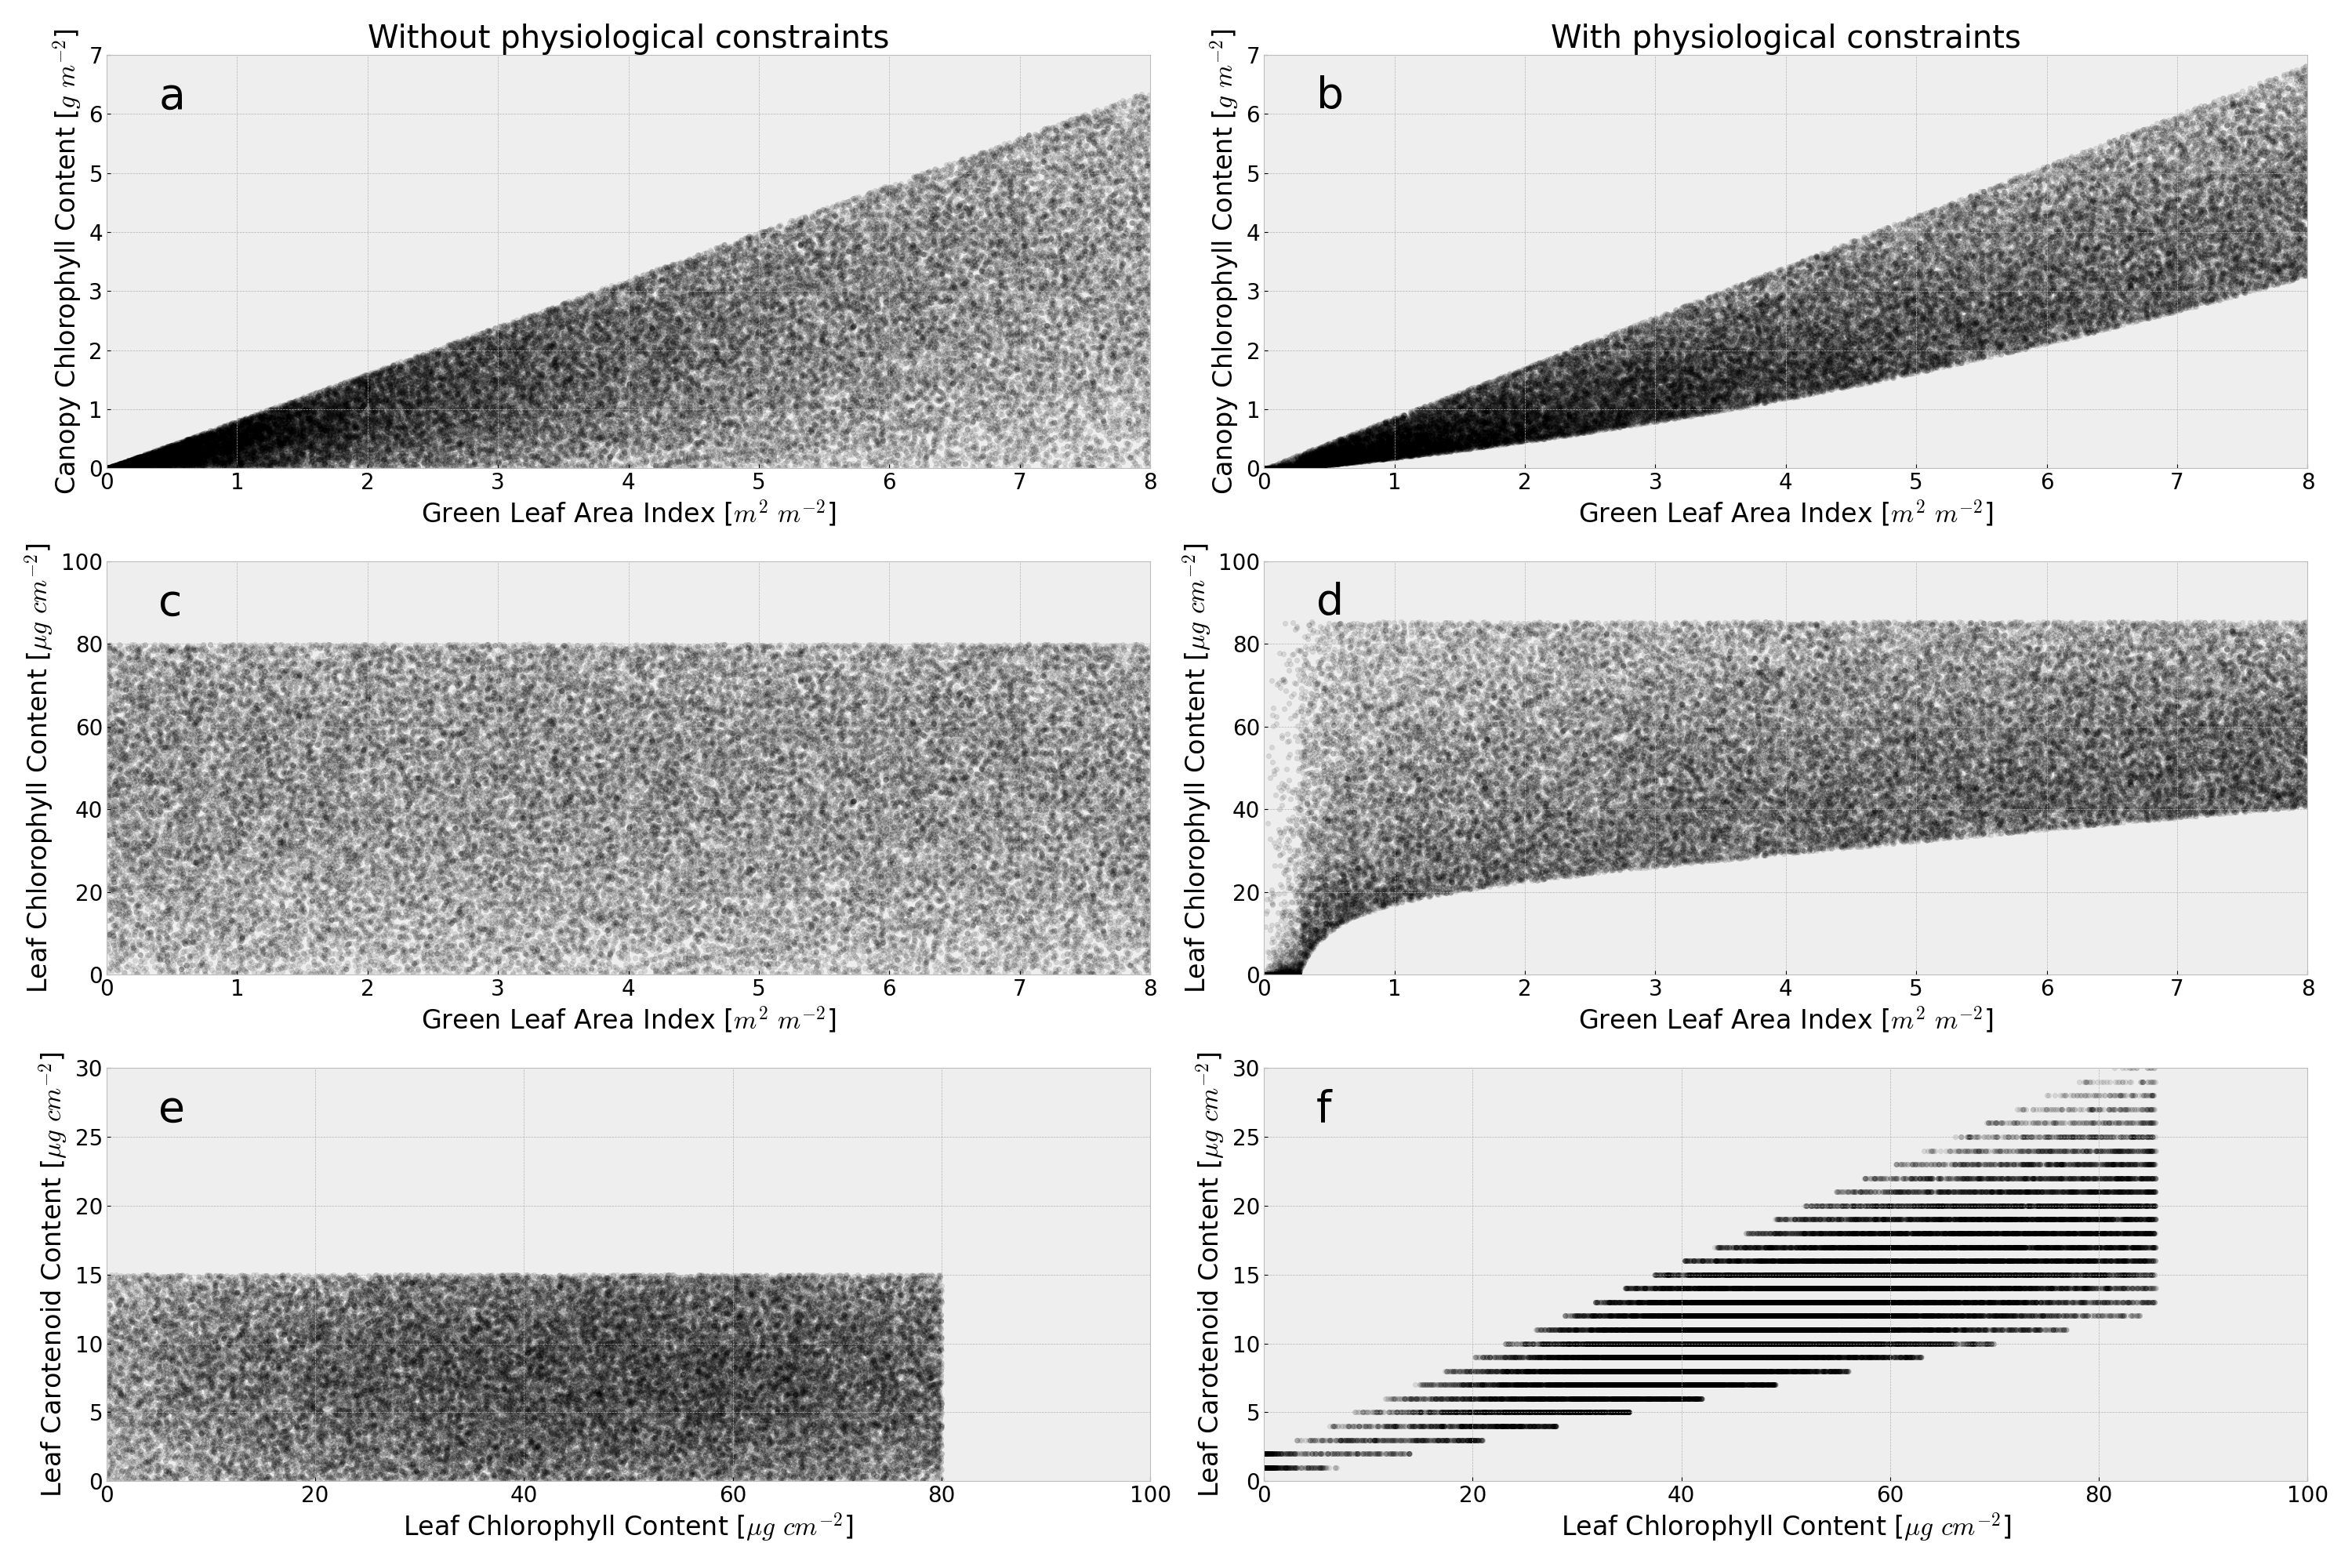
\includegraphics[width=1.0\textwidth]{constraints_in_lut.png}
    \caption[Implementation of physiological constraints in the LUT (N=50000) generated without phenological priors. (a) denotes the CCC-GLAI relationship without physiological constraints and (b) when the empirical relationship from Figure \ref{fig:lai-ccc-relationship} is enforced to redistribute CCC values. (c) shows the unrestricted relationship between Cab and GLAI and (d) the relationship when using the CCC values from (b). (e) and (f) show the redistribution of Car based on Cab (from (d)) as suggested by~\cite{wocher_rtm-based_2020}.]{Implementation of physiological constraints in the LUT (N=50000) generated without phenological priors. (a) denotes the CCC-GLAI relationship without physiological constraints and (b) when the empirical relationship from Figure \ref{fig:lai-ccc-relationship} is enforced to redistribute CCC values. (c) shows the unrestricted relationship between Cab and GLAI and (d) the relationship when using the CCC values from (b). (e) and (f) show the redistribution of Car based on Cab (from (d)) as suggested by~\cite{wocher_rtm-based_2020}.}
    \label{fig:constraints-in-lut}
\end{figure}


\subsubsection{Phenological Priors}
\label{subsubsec:phenological-constraints}
\paragraph{Dependency of GLAI on phenology}

As described in Section \ref{subsec:phenotyping-data}, CCC at the canopy as well as Cab and Car at the leaf scale are distributed based on GLAI (Figure \ref{fig:constraints-in-lut}b, d, f). GLAI in turn depends on phenology. From the SEON, MNI and Bramenwies datasets (see Table \ref{tab:phenotyping-datasources} and Sections \ref{subsubsec:seon-data} to \ref{subsubsec:bramenwies-data}) we analyzed the measured GLAI values using the 5, 50 and 95\% quantile. Analysis was carried out for all phenological stages (BBCH 0-99), as well as for GE-ET (BBCH 0-29), SE-EH (BBCH 31-59) and FL-PM (BBCH 61-99). The obtained descriptive statistics are shown in Table \ref{tab:glai-data}.

% add table with descriptive statistics of GLAI and CCC
\begin{table}[H]
\caption{Statistics of GLAI values in $m^2 m^{-2}$ for phenological macro stages and all stages derived from phenotyping data of winter wheat (N=909). Corresponding BBCH ranges are denoted in brackets.}
\label{tab:glai-data}
\begin{tabularx}{\textwidth}{p{4cm}p{1.8cm}p{1.8cm}p{1.8cm}p{0.8cm}}
\toprule
\textbf{Phenology} & \textbf{5\% Quantile} & \textbf{Median} & \textbf{95\% Quantile} & \textbf{N} \\ \midrule
GE-ET (0-29)  & 0.0   & 0 .6 &  2.0 & 189  \\
SE-EH (31-59)   & 0.5  & 4.2 & 6.5  & 661  \\
FL-PM (61-99)   & 0.3 & 6.3 &  8.0 & 166  \\
all (0-99)   & 0.0  &  3.8  & 8.0  & 909  \\ \bottomrule
\end{tabularx}
\end{table}

\paragraph{Dependency of phenology on air temperature}

Air temperature is an important driver of plant growth and phenological development~\citep{parent_temperature_2012, roth_high-throughput_2022}. We used the FIP field phenotyping data about the beginning of SE (BBCH 31) and EH (BBCH 59) to obtain descriptive statistics of the AGDD required for a winter wheat cultivar to reach these phenological stages. The descriptive statistics showing the 5, 50 and 95\% quantile are summarized in Table \ref{tab:bbch-agdd}.

\begin{table}[H]
\caption{AGDD statistics (in deg C) for begin of SE (BBCH 31) and EH(BBCH 59) derived from field phenotyping data at the FIP site.}
\label{tab:bbch-agdd}
\begin{tabularx}{\textwidth}{p{5cm}p{1.5cm}p{1.8cm}p{1.8cm}p{1.8cm}p{0.8cm}}
\toprule
\textbf{Phenological Stage}       & \textbf{BBCH Code}  & \textbf{5\% Quantile} & \textbf{Median} & \textbf{95\% Quantile} & \textbf{N} \\ \midrule
\textbf{Begin of Stem Elongation} & 31            &  737    & 803        & 870  & 357        \\
\textbf{End of Heading}           & 59            & 1382    & 1487       & 1602   & 1833      \\ \bottomrule
\end{tabularx}
\end{table}


\subsubsection{Radiative Transfer Modelling}
We used the PROSAIL RTM ~\citep{jacquemoud_prospectsail_2009} coupling the PROSPECT-D leaf RTM \citep{feret_prospect-d_2017} with the 4SAIL~\citep{verhoef_light_1984} canopy RTM to simulate winter wheat directional reflectance based on the proposed physiological and phenological priors (Sections \ref{subsubsec:physiological-constraints} and \ref{subsubsec:phenological-constraints}). PROSAIL is a one-dimensional RTM based on the turbid medium assumption meaning that canopies are treated as two-dimensional layers with scattering and absorbing particles. Three-dimensional structural effects are neglected. Viewing and illumination angles were set to scene-specific values. In PROSAIL, chlorophyll content is a leaf variable, Cab, (i.e., a variable of PROSPECT-D) given in $\mu g$ $cm^{-2}$. For scaling up to the canopy, we calculated CCC (in $g$ $m^{-2}$) based on GLAI (Equation \ref{eq:ccc-calc-rtm}).

Table \ref{tab:prosail-inputs} shows the leaf (PROSPECT-D) and canopy (4SAIL) parameters input into PROSAIL. The range of GLAI values denoted in Table \ref{tab:prosail-inputs} is set to the range found for all phenological phases (BBCH 0-99). For the phenological macro stages, the range of GLAI values is modified according to the 5-95\% quantile range denoted in Table \ref{tab:glai-data} (see Section \ref{subsubsec:phenological-constraints}) to integrate the phenological prior. In all phenological stages GLAI is distributed uniformly. Leaf parameters Cab and Car are redistributed based on GLAI as described in Section \ref{subsubsec:physiological-constraints} to ensure physiological plausibility of PROSAIL simulations. The remaining parameters are set to values provided by~\cite{wocher_rtm-based_2020} and~\cite{danner_efficient_2021}, which are also based on in-situ data including winter wheat samples.

\begin{table}[H]
\caption{Parameter ranges and distributions for the combined leaf (PROSPECT-D) and canopy (4SAIL) RTM (PROSAIL) without phenological priors applied to GLAI. The ranges are given for uniform distributions (range) or a truncated Gaussian distribution with mean and standard deviation denoted in brackets. Cab and Car are redistributed on GLAI as shown in Figure \ref{fig:constraints-in-lut} and explained in Section \ref{subsubsec:physiological-constraints}.}
\label{tab:prosail-inputs}
\begin{tabular}{@{}lllllll@{}}
\toprule
  \textbf{Trait}     & \textbf{Description}         & \textbf{Unit}           & \multicolumn{4}{l}{\textbf{Range}}              \\ \midrule
\multicolumn{7}{l}{\textbf{PROSPECT-D (Leaf)}}                                                                \\
\midrule
N      & Leaf Structure Parameter     & {[}-{]}                 & \multicolumn{4}{l}{1 - 2.5 (1.5, 0.2)}          \\
Cab    & Leaf Chlorophyll a+b Content & {[}$\mu g$ $cm^{-2}${]} & \multicolumn{4}{l}{redistributed based on GLAI} \\
Car    & Leaf Carotenoid Content      & {[}$\mu g$ $cm^{-2}${]} & \multicolumn{4}{l}{redistributed based on Cab}  \\
Cant   & Leaf Anthocyanin Content     & {[}$\mu g$ $cm^{-2}${]} & \multicolumn{4}{l}{0.0 - 5.0 (2.0, 0.8)}        \\
Cbrown & Brown Pigments               & {[}-{]}                 & \multicolumn{4}{l}{0 - 1}                       \\
Cw     & Equivalent Water Thickness   & {[}cm{]}                & \multicolumn{4}{l}{0 - 0.07 (0.04, 0.02)}       \\
Dm     & Dry Matter Content           & {[}$g$ $cm^{-2}${]}     & \multicolumn{4}{l}{0 - 0.01}                    \\
\midrule
\multicolumn{7}{l}{\textbf{4SAIL (Canopy)}}                                                                     \\
\midrule
GLAI   & Green Leaf Area Index        & {[}$m^2$ $m^{-2}${]}    & \multicolumn{4}{l}{0-8}                         \\
ALA    & Leaf Inclination Angle       & {[}deg{]}               & \multicolumn{4}{l}{30 - 70}                     \\
hspot  & Hot spot Parameter           & {[}-{]}                 & \multicolumn{4}{l}{0.01 - 0.5}                  \\
rsoil  & Soil Brightness Factor       & {[}-{]}                 & \multicolumn{4}{l}{0 - 1}                       \\
psoil  & Dry/ Wet Soil Factor         & {[}-{]}                 & \multicolumn{4}{l}{0 - 1}                       \\ \bottomrule
\end{tabular}
\end{table}

Thus, for each S2 scene we generated four lookup tables (LUTs): Three LUTs for the phenological macro stages (GE-ET, SE-EH, FL-PM) and a single LUT for all stages (BBCH 0-99). We used a fully randomized sampling scheme to generate input pairs of leaf and canopy parameters from Table \ref{tab:prosail-inputs} to run PROSAIL in forward mode. After running PROSAIL, we carried out further post-processing: We discarded simulated spectra that had a physiologically unrealistic blue shift of the green reflectance peak as proposed by ~\cite{wocher_rtm-based_2020}. In detail,~\cite{wocher_rtm-based_2020} analyzed data from handheld field spectrometers, airborne hyperspectral imaging sensors and the ANGERS leaf optical dataset~\citep{jacquemoud_angers_2003}. They observed that green reflectance peaks of vegetation do not occur at wavelengths < 547 nm. PROSAIL, however, sometimes simulates vegetation spectra in which the green peak is shifted towards shorted wavelengths (i.e., < 547 nm). This may be an indication of physiologically implausible input parameter combinations or a modeling artifact. Due to inadmissible shifts of the green peak, we discarded around 5\% of the simulated S2 spectra. This is clearly lower than the number of 23\% of invalid spectra reported by~\cite{wocher_rtm-based_2020} suggesting that physiological priors reduce the amount of implausible PROSAIL spectra.

The remaining 1 nm PROSAIL outputs were resampled to the spectral response functions of S2A and S2B provided by ESA. Input parameters and simulated S2 spectra were stored in LUTs for RTM inversion. 

\subsection{Model Inference}
\label{subsec:model-inference}

For inference on S2 imagery, three scenarios were run: The first scenario setup uses a single RTM parametrization for the entire growing season (NO-PHENO). In the second scenario we use AGDDs for estimating the onset of phenological stages and use the LUT of the macro stage (AGDD-PHENO). The third scenario is essentially the same as the second but includes spatial detail from S2 pixel-based cost function values (see Section \ref{subsubsec:pheno-from-s2}) to test if differences in phenological transitions can be detected within the field parcels (AGDD-S2-PHENO).

\subsubsection{RTM Inversion}
For each S2 scene we obtained GLAI, CCC and hence Cab using the simulated S2 LUTs. We took the median of the $n$ best solutions in terms of the smallest cost function values between observed and simulated S2 spectra. As cost function we used the root mean squared error (RMSE) between S2 observed ($p$) and PROSAIL simulated spectra ($q$) considering all $\lambda_1, ...., \lambda_m$ spectral bands of S2 used ($m=9$, see Section \ref{subsec:rs-data}):

\begin{equation}
    RMSE = \sqrt{\frac{\sum_{\lambda_i = 1}^{\lambda_m}(p(\lambda_i) - q(\lambda_i))^2}{m}}
\end{equation}

Table \ref{tab:inv-setup} shows the configurations used for the phenological phases (scenarios AGDD-PHENO and AGDD-S2-PHENO) and the NO-PHENO scenario. The configurations were obtained from systematic testing of different cost functions, LUT sizes and number of solutions of the inversion (see Table \ref{tab:prosail-inv-settings} in \ref{Appendix}). We optimized for enhancing the correlation between modeled and in-situ observed GLAI values in terms of Pearson's R-square $R^2$.

\begin{table}[H]
\caption{Setup of the LUT-based inversion for the phenological phases including the cost function, LUT size, and the scenario the LUT was used for (RMSE: root mean squared error, MAE: mean absolute error). The BBCH ranges are denoted in brackets}
\label{tab:inv-setup}
\begin{tabularx}{\textwidth}{p{4cm}p{1.8cm}p{1.8cm}p{1.8cm}p{2.8cm}}
\toprule
\textbf{Phenology} & \textbf{Cost Function} & \textbf{LUT size} & \textbf{No. Solutions}  & \textbf{Scenarios}\\ \midrule
GE-ET (0-29)                 & RMSE          & 10000              & 100        & AGDD-PHENO, AGDD-S2-PHENO         \\
SE-EH (31-59)                & MAE           & 50000              & 5000   & AGDD-PHENO, AGDD-S2-PHENO             \\
FL-PM (61-99)                & MAE           & 50000              & 5000    & AGDD-PHENO, AGDD-S2-PHENO            \\
all (0-99)                 & MAE           & 50000              & 5000     & NO-PHENO           \\ \bottomrule
\end{tabularx}
\end{table}

\subsubsection{Phenology Retrieval}
\label{subsubsec:pheno-from-s2}
In the NO-PHENO scenario a single RTM parametrization was used for all S2 scenes to derive GLAI and CCC. In the other two scenarios we had to determine the phenological macro stage to select the appropriate LUT for RTM inversion. Figure \ref{fig:workflow-phenology} highlights the procedure for a hypothetical S2-derived trait time series. The red rectangles define the AGDD ranges identified from field phenotyping (Table \ref{tab:bbch-agdd}) where a switch between the phenological stages most likely occurs. In the AGDD-PHENO scenario we used the median AGDD obtained from Table \ref{tab:bbch-agdd} to switch between the phenological phases (dashed lines in Figure \ref{fig:workflow-phenology}). In the AGDD-S2-PHENO scenario we used the value of cost function of the RTM inversion in addition. I.e., in the AGDD window of beginning of SE (BBCH31) we compared the median cost function value from inverting the LUT for the tillering phase (GE-ET, BCCH 0-29) with the value obtained from SE-EH (BBCH 31-59). If the latter was lower, we switched from tillering into stem elongation. Otherwise the observation remained in the tillering phase until either the cost function value from stem elongation was lower or the end of the critical AGDD was reached. In that case, a switch was forced. In case no S2 scene was available we used the same procedure as in AGDD-PHENO.

\begin{figure}[H]
    \centering
    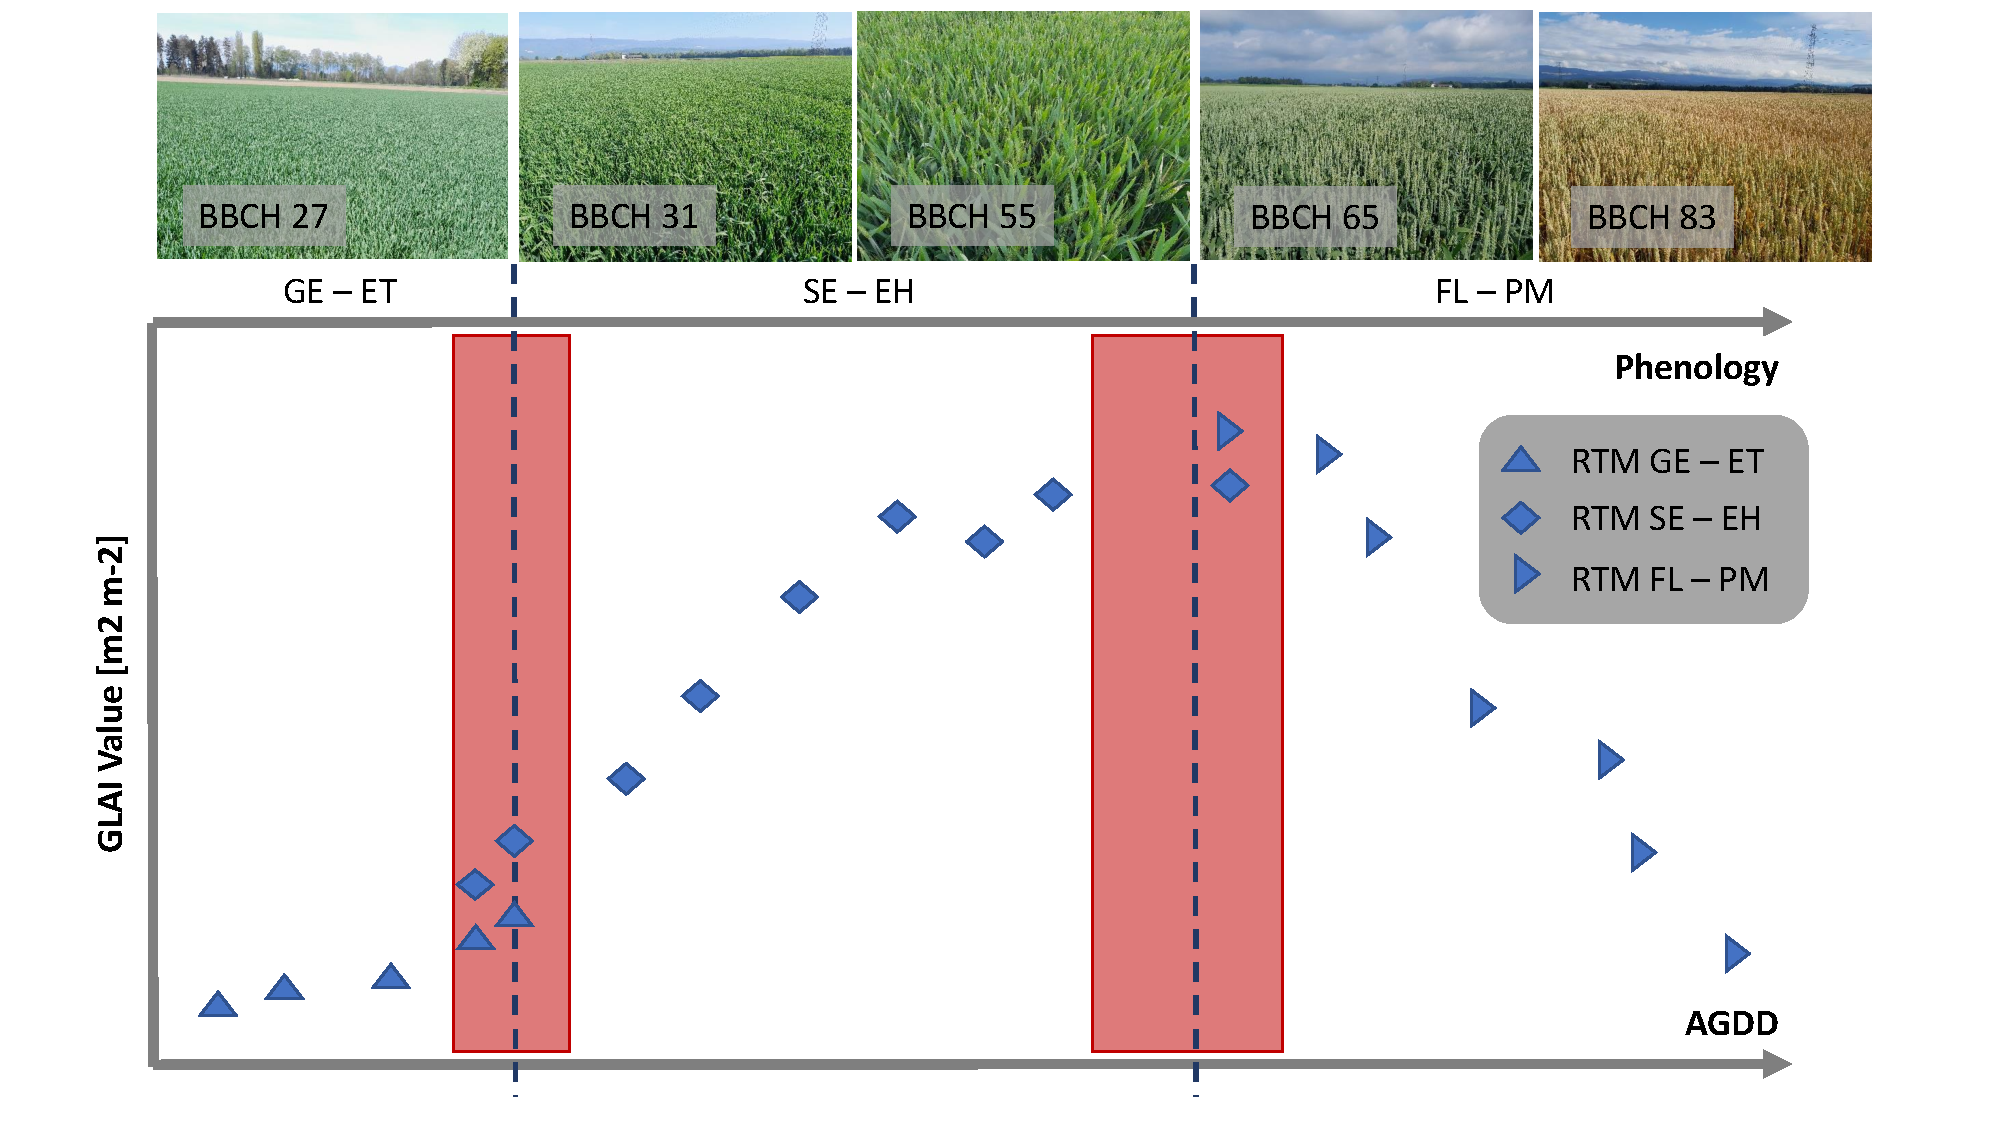
\includegraphics[width=1.0\textwidth]{Workflow_Phenology.pdf}
    \caption[Proposed workflow for estimating the transition between main phenological stages in winter wheat based on accumulated growing degree days (AGDD) and GLAI trajectories from RTM inversion. The red rectangles denote AGDD windows where transitions from tillering to stem elongation and from heading to flowering most likely occur based on phenotyping experiments. The dashed lines denote the median AGDD for these transitions. Examples of winter wheat canopies at different development stages (expressed in BBCH codes) are shown in the top row in addition.]{Proposed workflow for estimating the transition between main phenological stages in winter wheat based on accumulated growing degree days (AGDD) and GLAI trajectories from RTM inversion. The red rectangles denote AGDD windows where transitions from tillering to stem elongation and from heading to flowering most likely occur based on phenotyping experiments. The dashed lines denote the median AGDD for these transitions. Examples of winter wheat canopies at different development stages (expressed in BBCH codes) are shown in the top row in addition.}
    \label{fig:workflow-phenology}
\end{figure}

\subsection{Model Validation}
\label{subsec:model-validation}

\subsubsection{On-farm trial data processing}
Independent measurements of GLAI, CCC and BBCH were recorded at weekly to bi-weekly intervals at on-farm locations in Switzerland (see Figure \ref{fig:overview-map} and Table \ref{tab:site_characteristics}) using the methods described in Section \ref{subsec:in-situ-data-processing}. These measurements are used to test the accuracy of models calibrated on field phenotyping data applied to S2 imagery at the landscape scale (see Section \ref{subsubsec:comparison-sat-insitu}).

\subsubsection{Comparison of satellite and in-situ data}
\label{subsubsec:comparison-sat-insitu}
Modelled GLAI, CCC and phenological macro stages were compared against on-farm validation data (see Section \ref{subsec:on-farm-trials}). We used a maximum difference of 20 GDD between in-situ sampling dates and S2 overpasses which corresponds to a maximum temporal difference of one up to a couple of days depending on the time of the year. For spatial intersection, we constructed a circle with 10 m radius around the point coordinate of the in-situ measurement. We used the mean of all S2 pixels that overlapped this circle. This is to ensure that the influence of uncertainties in the positional accuracy of both data sources is minimized.

We then calculated common error metrics including the root mean squared error (RMSE), normalized RMSE (nRMSE), normalized absolute median deviation (NMAD) and $R^2$ to compare modelled GLAI and CCC to in-situ samples. We treated the retrieval of the three phenological macro stages as a classification problem, i.e., a segmentation of the growing season into three stages, in which the true phenological macro stage obtained from the BBCH ratings served as target class label. We calculated the confusion matrix, the F1-score per phenological stage, i.e., per class, and an adjusted F1-score accounting for class imbalances to quantify model performance using phenological data from 2022.
For a single class classification problem, i.e., a single phenological phase, the F1-score is the harmonic mean of precision (positive predictive value) and recall (true positive rate) calculated from the number of true and false positives (tp, fp), as well as true and false negatives (tn, fn).

\begin{equation}
    precision = \frac{tp}{tp + fp}
\end{equation}

\begin{equation}
    recall = \frac{tp}{tp + fn}
\end{equation}

\begin{equation}
    F1\-score = \frac{2 \times precision \times recall}{precision + recall}
\end{equation}
For a multi-class classification problem as in this study, the adjusted F1-score is calculated from the F1-scores per class weighted by the number of samples per class. The adjusted F1-score is thus a measure for the overall performance of the phenological model.
Error metrics were provided for all three experimental setups to test the effect of phenological priors on RTM inversion accuracy and determine the most accurate method for phenology estimation.

\section{Results}
\label{sec:results}
% \subsection{Validation of raw S2 GLAI observations against in-situ GLAI}

Figure \ref{fig:s2-obs-scatter-plots} shows the raw \gls{S2} \gls{GLAI} observations plotted against in-situ measured \gls{GLAI} with a maximum temporal offset of one day. The \gls{RMSE} was about 1.16 $m^2$ $m^{-2}$ (\gls{nRMSE} 18.92\%) with a bias of 1.87 $m^2$ $m^{-2}$. The raw \gls{S2} \gls{GLAI} observations explained 64\% of the variability in the in-situ values. The raw \gls{S2} \gls{GLAI} values showed a clear underestimation of in-situ \gls{GLAI} > 5 $m^2$ $m^{-2}$ in 2022 (blue dots in Figure \ref{fig:s2-obs-scatter-plots}) as well as three isolated outliers in 2023 (cross markers) for in-situ \gls{GLAI} values between 2 and 3 $m^2$ $m^{-2}$. Due to high cloud cover, only 8 out of 55 available observations for validation were recorded in 2023. Therefore, no year effects could be studied. The same applies to the phenological macro-stages for which not enough data was available to compute robust error statistics.

\begin{figure}[H]
    \centering
    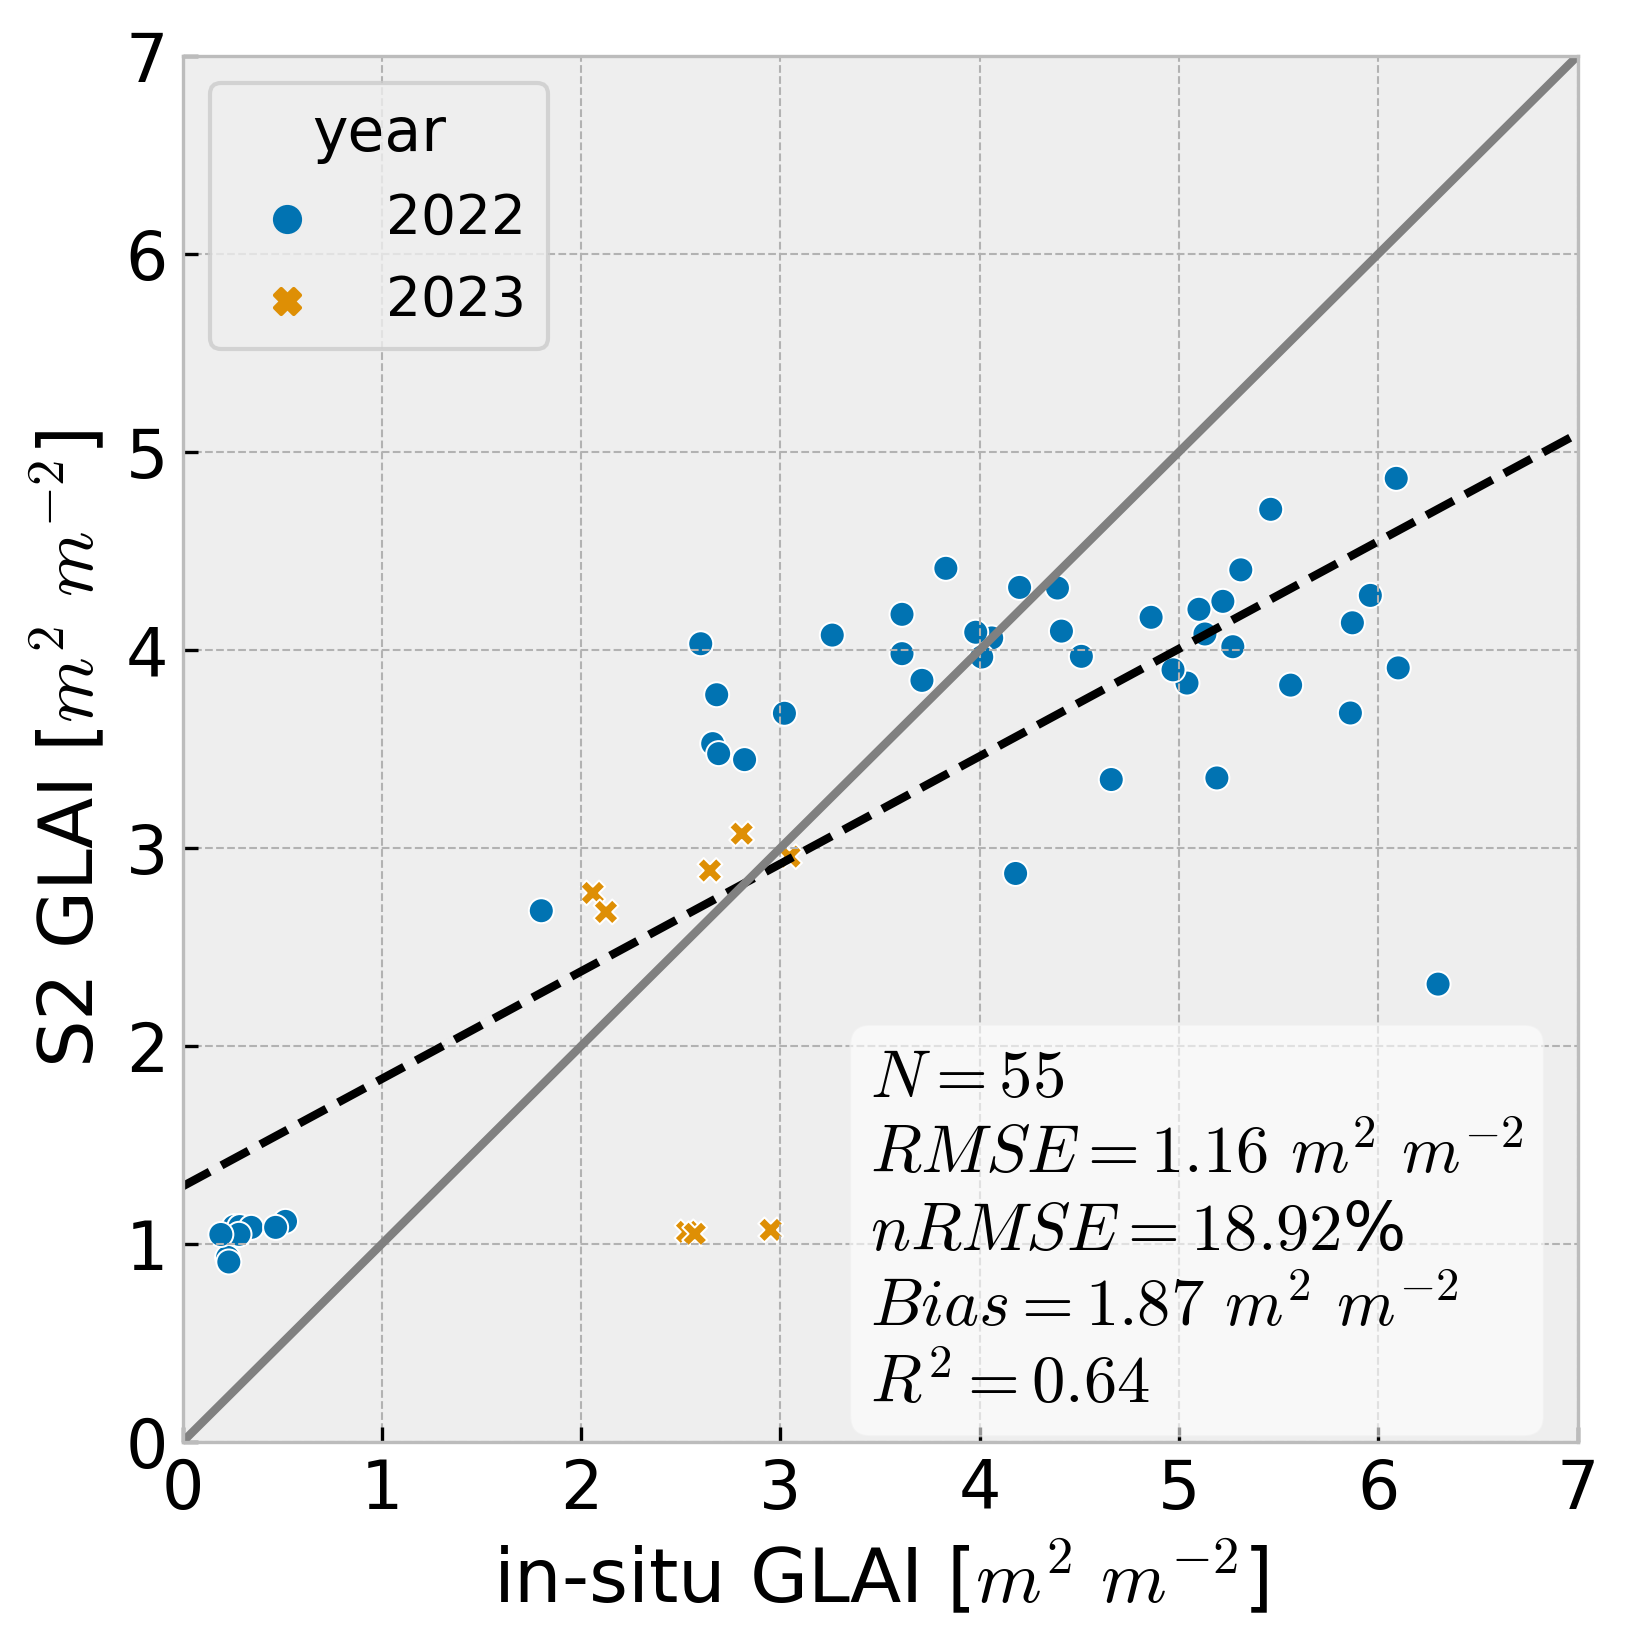
\includegraphics{s2_glai-obs_validation.png}
    \caption{Scatter plots of S2 observed and in-situ measured GLAI at the validation sites using data from 2022 and 2023. The oblique solid lines denotes the desired 1:1 fit; the dashed line denotes the linear regression line between S2 observed and in-situ measured \gls{GLAI} values. N = 55. The years are color-coded.}
    \label{fig:s2-obs-scatter-plots}
\end{figure}

\subsection{Validation of reconstructed GLAI time series against in-situ GLAI}
Similar to Figure \ref{fig:s2-obs-scatter-plots}, scatter plots of reconstructed GLAI (i.e., \gls{DRC} and baseline \gls{GLAI}) at hourly and daily resolution against in-situ measured \gls{GLAI} are displayed in Figure~\ref{fig:glai-scatter-plots} (N = 178). Figure~\ref{fig:glai-scatter-plots} (a-c) shows the results of the proposed \gls{DRC} GLAI time series, and (d) the baseline \gls{GLAI} results which are available in daily resolution, only. The error statistics are listed in Table~\ref{tab:error-stats}.

All models revealed a tendency to overestimate low in-situ \gls{GLAI} (< 1.0 $m^2$ $m^{-2}$). The baseline (Figure~\ref{fig:glai-scatter-plots}d) clearly underestimated in-situ \gls{GLAI} values > 5.0 $m^2$ $m^{-2}$. All models performed similar in terms of \gls{RMSE}, \gls{nRMSE} and \gls{R2} (Table~\ref{tab:error-stats}). The hourly asymptotic \gls{DRC} \gls{GLAI} had the smallest \gls{RMSE} (0.98 $m^2$ $m^{-2}$) closely followed by the daily asymptotic and non linear \gls{DRC} \gls{GLAI} (\gls{RMSE} around 0.99  $m^2$ $m^{-2}$, \gls{nRMSE} around 15\%). The highest \gls{RMSE} was observed for the Wang Engels \gls{DRC} \gls{GLAI} at hourly resolution (1.12  $m^2$ $m^{-2}$, \gls{nRMSE}: 17.43\%). The baseline \gls{GLAI} had a slightly lower \gls{RMSE} (1.05  $m^2$ $m^{-2}$, \gls{nRMSE}: 16.27\%) than the daily Wang Engels \gls{DRC} \gls{GLAI} (1.06  $m^2$ $m^{-2}$). A similar picture revealed \gls{R2} which ranged between 0.54 (Wang Engels hourly \gls{DRC} \gls{GLAI}) and 0.70 (non linear daily \gls{DRC} \gls{GLAI}). The highest bias was observed for the baseline \gls{GLAI} (1.66  $m^2$ $m^{-2}$). This was higher than for the \gls{DRC} \gls{GLAI} and more than two times larger than the smallest bias (0.73  $m^2$ $m^{-2}$) obtained from the hourly Wang Engels \gls{DRC} \gls{GLAI} which had the lowest bias.

\begin{figure}[H]
    \centering
    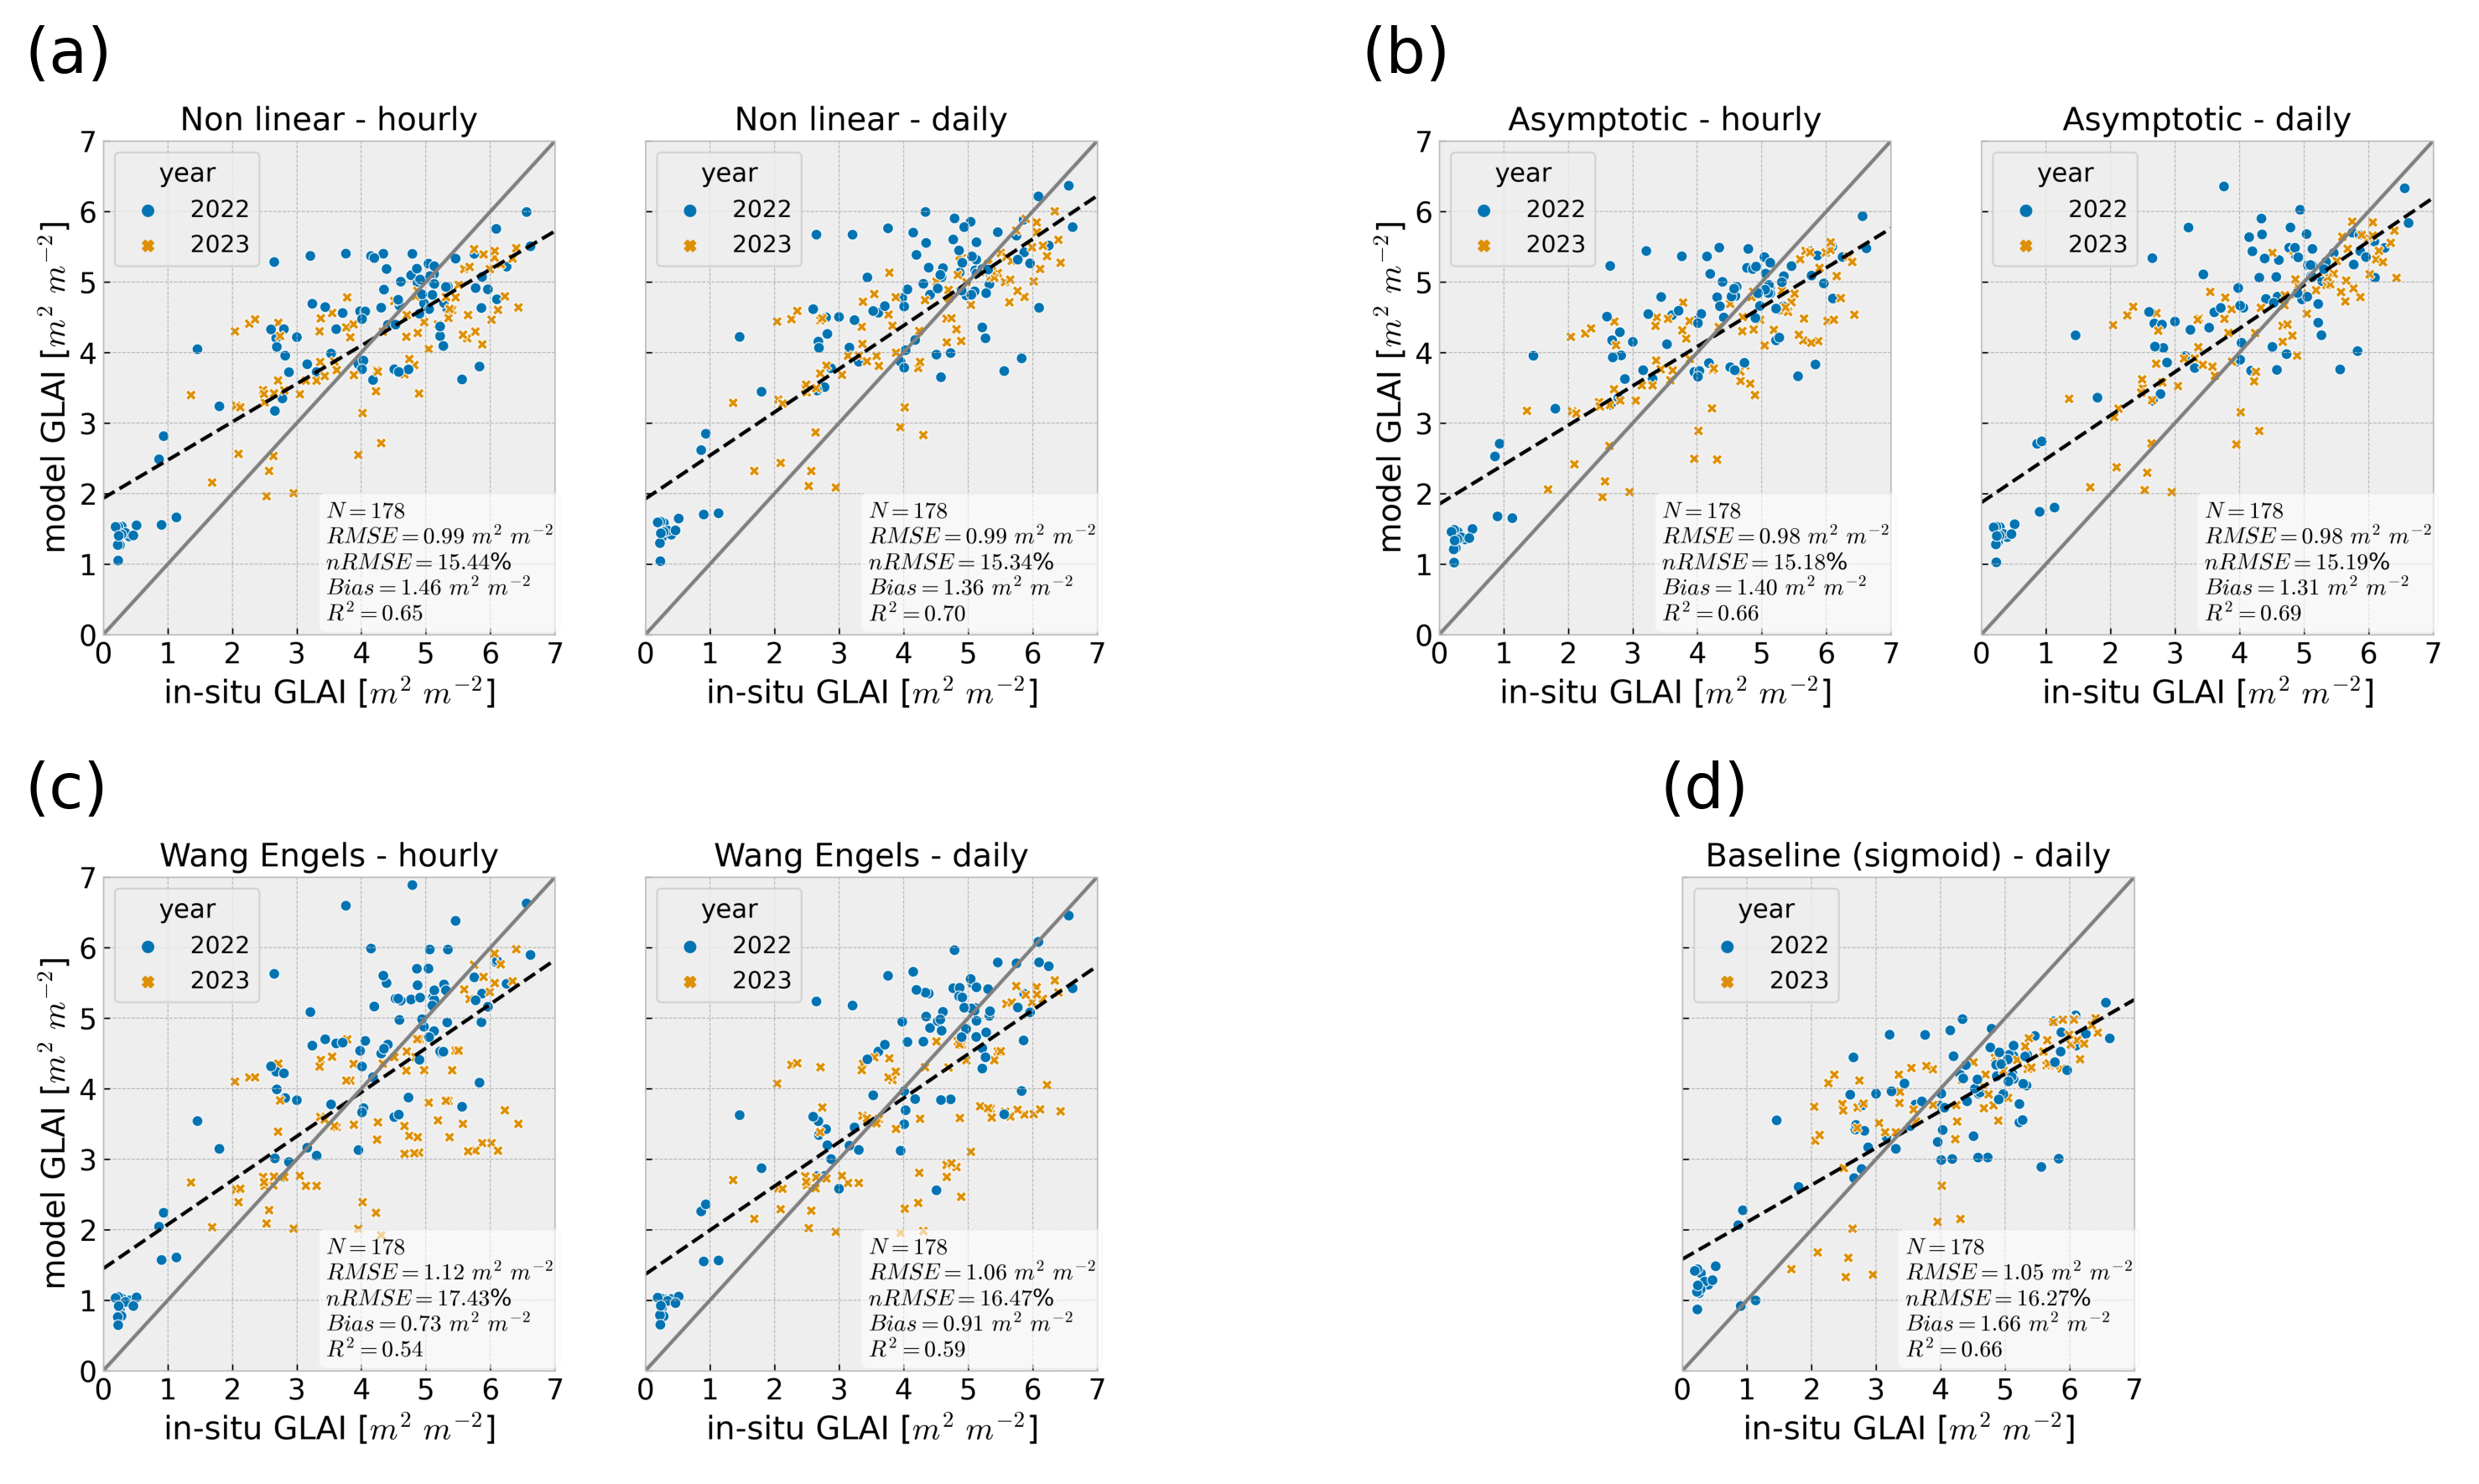
\includegraphics[width=\textwidth]{glai_scatter_plots.png}
    \caption{Scatter plots between reconstructed \gls{DRC} (a-c) and baseline (d) \gls{GLAI} and in-situ \gls{GLAI} at the validation sites using data from 2022 and 2023 (color-coded). For each \gls{DRC} \gls{GLAI}, the results using hourly and daily mean air temperature are shown (a-c). The baseline \gls{GLAI} is only available in daily resolution (d). The oblique solid line denotes the desired 1:1 fit and the dashed line the linear regression line between reconstructed and in-situ \gls{GLAI} values. N = 178.}
    \label{fig:glai-scatter-plots}
\end{figure}

\begin{table}[H]
\caption{Error statistics of reconstructed and in-situ \gls{GLAI} values (N = 178). \gls{RMSE} and bias are given in $m^2$ $m^{-2}$, \gls{nRMSE} in percent and \gls{R2} is dimensionless.}
\label{tab:error-stats}
\centering
\begin{tabular}{@{}llllll@{}}
\toprule
model                        & resolution & \gls{RMSE}          & \gls{nRMSE}         & Bias          & \gls{R2}            \\ \midrule
\multirow{2}{*}{Non linear} & hourly      & 0.99          &  15.44 & 1.46          & 0.65          \\
                             & daily       & 0.99          & 15.34 & 1.36          & 0.70 \\
\multirow{2}{*}{Asymptotic}  & hourly      & 0.98 & 15.17 & 1.40          & 0.66          \\
                             & daily       & 0.98 & 15.19 & 1.31          & 0.69          \\
\multirow{2}{*}{Wang Engels}  & hourly      & 1.12          & 17.43          & 0.73 & 0.54          \\
                             & daily       & 1.06          & 16.47          & 0.91          & 0.59          \\
Baseline (sigmoid)                      & daily       & 1.05          & 16.27          & 1.66          & 0.66          \\ \bottomrule
\end{tabular}
\end{table}

\subsubsection{Effect of the years}
Error statistics by year are shown in Table~\ref{tab:error-stats-years}. Arrows in table indicate whether a metric value remain unchanged ($\rightarrow$), decrease ($\downarrow$), or increased ($\uparrow$) from 2022 to 2023. For all models and temporal resolutions, the relative error was higher and $R^2$ lower in 2023 (N = 82) than 2022 (N = 96). In 2022, nRMSE values ranged from 13.04 (Wang Engels daily) to 16.72\% (non linear daily), while $R^2$ took values between 0.74 (baseline) and 0.8 (Wang Engels daily). In 2023, nRMSE values were in the range between 17.16 (asymptotic daily) and 25.62\% (Wang Engels hourly) with $R^2$ between 0.3 (Wang Engels hourly) and 0.62 (non linear daily). The RMSE was higher in 2023 than 2022 in four cases (asymptotic hourly, Wang Engels hourly and daily, and the baseline), unchanged in one case (non linear hourly), and decreased in the remaining two cases (non linear daily and asymptotic daily). The highest RMSE was obtained from the hourly Wang Engels \gls{DRC} in 2023 (1.30 $m^2$ $m^{-2}$, value in 2022: 0.94 $m^2$ $m^{-2}$), the lowest for the Wang Engels \gls{DRC} in 2022 (0.84 $m^2$ $m^{-2}$, value in 2023: 1.27 $m^2$ $m^{-2}$). The bias decreased in all cases in 2023 compared to 2022 except the Wang Engels \gls{DRC}: Here, the bias increased from 0.83 to 1.10 $m^2$ $m^{-2}$ (hourly) and from 0.90 to 1.22 $m^2$ $m^{-2}$ (daily).

%In 2022 (N = 96), \gls{DRC} and baseline \gls{GLAI} accuracy was mostly higher than in 2023 (N = 82). In 2022, \gls{R2} ranged from 0.74 for the baseline to 0.8 for the daily Wang Engels \gls{DRC} \gls{GLAI} (Table~\ref{tab:error-stats-2022}). In 2023, \gls{R2} values were lower ranging between 0.3 (Wang Engels hourly \gls{DRC} \gls{GLAI}) and 0.62 (non linear daily \gls{DRC} \gls{GLAI}). The bias was mostly higher in 2022 ranging between 0.83 $m^2$ $m^{-2}$ for the Wang Engels hourly \gls{DRC} \gls{GLAI} to 1.96 $m^2$ $m^{-2}$ for the baseline \gls{GLAI}. In 2023, the bias was highest for the daily Wang Engels \gls{DRC} \gls{GLAI} (1.22 $m^2$ $m^{-2}$) and lowest for the daily asymptotic \gls{DRC} \gls{GLAI} (0.96 $m^2$ $m^{-2}$).

%Overall, the Wang Engels \gls{DRC} \gls{GLAI} showed the most pronounced differences between the years. In 2022, the \gls{RMSE} of the Wang Engels \gls{DRC} \gls{GLAI} was about 0.94 and 0.84 $m^2$ $m^{-2}$ for the hourly and daily model, respectively (\gls{nRMSE} around 15 and 13\%). In 2023 (N = 82), the \gls{RMSE} decreased to 1.30 and 1.27 $m^2$ $m^{-2}$ (nRMSE: 24 and 25\%, respectively).

%\begin{table}[H]
%\caption{Error statistics of reconstructed and in-situ \gls{GLAI} values in 2022 (N = 96). \gls{RMSE} and bias are given in $m^2$ $m^{-2}$, \gls{nRMSE} in percent and \gls{R2} is dimensionless.}
%\label{tab:error-stats-2022}
%\centering
%\begin{tabular}{@{}llllll@{}}
%\toprule
%model                        & resolution & \gls{RMSE} & \gls{nRMSE} & Bias & \gls{R2}   \\ \midrule
%\multirow{2}{*}{Non linear} & hourly     & 0.99 & 15.44 & 1.71 & 0.75 \\
%                             & daily      & 1.07 & 16.72 & 1.64 & 0.75 \\
%\multirow{2}{*}{Asymptotic}  & hourly     & 0.96 & 14.98 & 1.66 & 0.77 \\
%                             & daily      & 1.06 & 16.47 & 1.60 & 0.75 \\
%\multirow{2}{*}{Wang Engels}  & hourly     & 0.94 & 14.64 & 0.83 & 0.77 \\
%                             & daily      & 0.84 & 13.04 & 0.90 & 0.80 \\ 
%Baseline (sigmoid)           & daily      & 1.03 & 15.97 & 1.96 & 0.74 \\ \bottomrule
%\end{tabular}
%\end{table}

\begin{table}[H]
    \centering
    \caption{Error statistics of reconstructed and in-situ \gls{GLAI} values in 2022 (N = 96) and 2023 (N = 82). The arrows indicate the change in the metrics from 2022 to 2023: $\uparrow$ means the value increased in 2023 compared to 2022, $\downarrow$ it decreased, and $\rightarrow$ it remained unchanged. \gls{RMSE} and bias are given in $m^2$ $m^{-2}$, \gls{nRMSE} in percent and \gls{R2} is dimensionless.}
    \label{tab:error-stats-years}
\begin{tabular}{@{}llllllllllllll@{}}
\toprule
model                        & resolution & \multicolumn{3}{l}{RMSE} & \multicolumn{3}{l}{nRMSE} & \multicolumn{3}{l}{Bias} & \multicolumn{3}{l}{$R^2$} \\ \midrule
                             &            & 2022    & 2023     &             & 2022     & 2023     &            & 2022   & 2023   &             & 2022   & 2023   &     \\ \cmidrule(l){2-14} 
\multirow{2}{*}{Non linear}  & hourly     & 0.99  & 0.99  & $\rightarrow$ & 15.44  & 19.58  & $\uparrow$  & 1.71 & 1.18 & $\downarrow$ & 0.75 & 0.49 & $\downarrow$ \\
                             & daily      & 1.07  & 0.87  & $\downarrow$  & 16.72  & 17.18  & $\uparrow$  & 1.64 & 1.01 & $\downarrow$ & 0.75 & 0.62 & $\downarrow$ \\ \cmidrule(l){2-14} 
\multirow{2}{*}{Asymptotic}  & hourly     & 0.96  & 0.99  & $\uparrow$    & 14.98  & 19.52  & $\uparrow$  & 1.66 & 1.14 & $\downarrow$ & 0.77 & 0.50 & $\downarrow$  \\
                             & daily      & 1.06  & 0.87  & $\downarrow$  & 16.47  & 17.16  & $\uparrow$  & 1.60 & 0.96 & $\downarrow$ & 0.75 & 0.60 & $\downarrow$  \\ \cmidrule(l){2-14} 
\multirow{2}{*}{Wang Engels} & hourly     & 0.94  & 1.30  & $\uparrow$    & 14.64  & 25.62  & $\uparrow$  & 0.83 & 1.10 & $\uparrow$   & 0.77 & 0.30 & $\downarrow$  \\
                             & daily      & 0.84  & 1.27  & $\uparrow$    & 13.04  & 25.02  & $\uparrow$  & 0.90 & 1.22 & $\uparrow$   & 0.80 & 0.33 & $\downarrow$  \\ \cmidrule(l){2-14} 
\shortstack{Baseline\\(sigmoid)} & daily      & 1.03  & 1.07  & $\uparrow$    & 15.97  & 22.55  & $\uparrow$  & 1.96 & 1.21 & $\downarrow$ & 0.74 & 0.48 & $\downarrow$  \\ \bottomrule
\end{tabular}
\end{table}


%\begin{table}[H]
%\caption{Error statistics of reconstructed and in-situ \gls{GLAI} values in 2023 (N = 82). \gls{RMSE} and bias are given in $m^2$ $m^{-2}$, \gls{nRMSE} in percent and \gls{R2} is dimensionless.}
%\label{tab:error-stats-2023}
%\centering
%\begin{tabular}{@{}llllll@{}}
%\toprule
%model                        & resolution & \gls{RMSE} & \gls{nRMSE} & Bias & \gls{R2}   \\ \midrule
%\multirow{2}{*}{Non linear}  & hourly     & 0.99 & 19.58 & 1.18 & 0.49 \\
%                             & daily      & 0.87 & 17.18 & 1.01 & 0.62 \\
%\multirow{2}{*}{Asymptotic}  & hourly     & 0.99 & 19.52 & 1.14 & 0.50 \\
%                            & daily      & 0.87 & 17.16 & 0.96 & 0.60 \\
%\multirow{2}{*}{Wang Engels} & hourly     & 1.30 & 25.62 & 1.10 & 0.30 \\
%                             & daily      & 1.27 & 25.02 & 1.22 & 0.33 \\
%Baseline (sigmoid)           & daily      & 1.07 & 22.55 & 1.21 & 0.48 \\ \bottomrule
%\end{tabular}
%\end{table}

\subsubsection{Effect of phenology}
The \gls{GLAI} reconstruction errors were dependent on the phenological macro-stage. Figure~\ref{fig:glai-errors-phenology} shows the error measures for \gls{BBCH} macro stages 30-39 (stem elongation), and 50-59 (heading) for the \gls{DRC} and baseline with daily \gls{GLAI} output. There were too few in-situ data for the booting stage (N = 5) available, so we restricted our analysis to stem elongation (N = 136) and heading (N = 37). For these stages, the baseline \gls{GLAI} exhibited the largest bias (1.6 and 1.2 $m^2$ $m^{-2}$, respectively). During heading, the baseline \gls{GLAI} also showed largest \gls{RMSE} (around 1.2 $m^2$ $m^{-2}$) and its bias was almost twice as high as in the \gls{DRC} \gls{GLAI} (bias around 0.6 $m^2$ $m^{-2}$). The difference in \gls{R2} was less pronounced; the \gls{DRC} and baseline \gls{GLAI} had a high \gls{R2} in stem elongation (0.55 to 0.73), which decreased significantly during heading (0.05 to 0.15). Overall, the differences between the three \gls{DRC} \gls{GLAI} models were less pronounced than the difference between these models and the baseline \gls{GLAI}.

\begin{figure}[H]
    \centering
    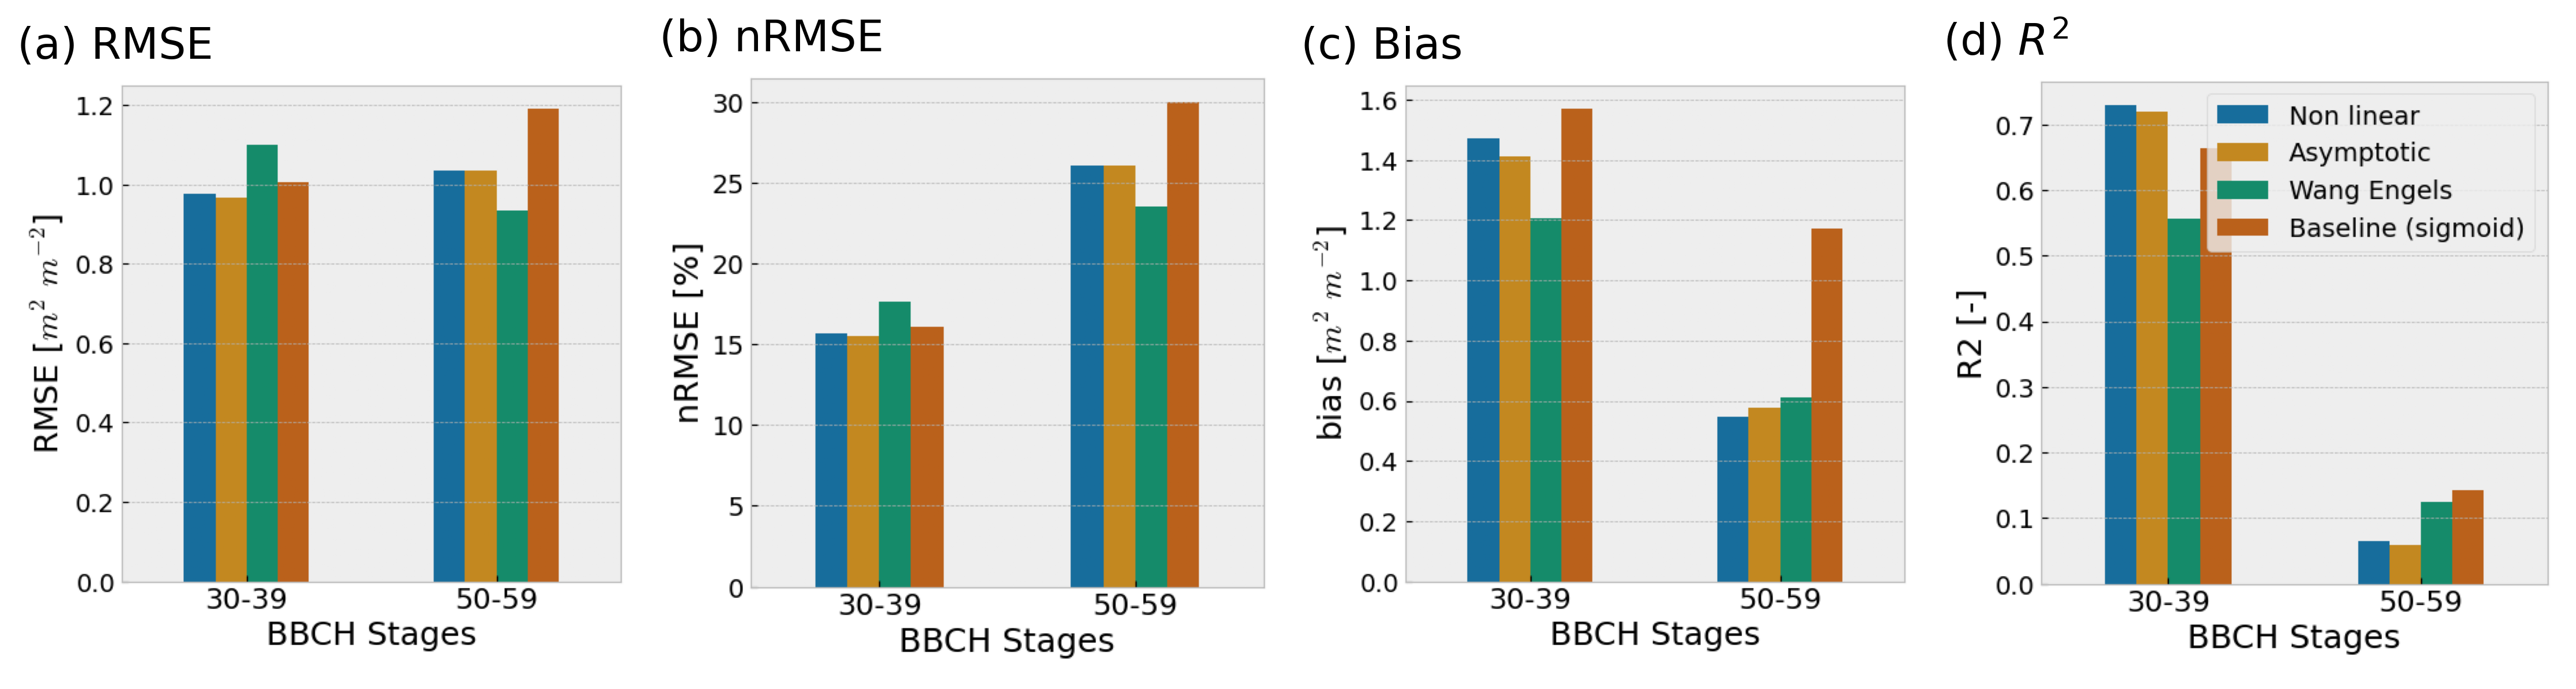
\includegraphics[width=\textwidth]{glai_daily-error_plots-bbch.png}
    \caption{Reconstructed versus in-situ \gls{GLAI} error statistics per BBCH macro-stage and model. Only the results of the daily \gls{DRC} \gls{GLAI} are shown.}
    \label{fig:glai-errors-phenology}
\end{figure}

\subsubsection{Time series reconstruction}

Figure~\ref{fig:glai-trajectories} visualizes the reconstructed median \gls{DRC} and baseline \gls{GLAI} time series at daily resolution in \gls{DAS} per field parcel and year (see also Figure~\ref{fig:map-validation-sites}). The spatial in-field variability obtained from each model is shown as filled areas color-coded by model. The in-situ \gls{GLAI} values are plotted as blue dots to allow comparison of reconstructed versus measured in-field heterogeneity and temporal dynamics. Both, \gls{DRC} and baseline \gls{GLAI} show an increase in \gls{GLAI} from the beginning of the stem elongation to the end heading, which largely reflects the dynamics of the in situ data.

The asymptotic (dotted green) and non linear (solid golden) \gls{DRC} \gls{GLAI} were able to accurately reconstruct in-situ \gls{GLAI} spatial variability and reflect the temporal trajectories of the in-situ \gls{GLAI} values. These models were able to represent the higher in-situ \gls{GLAI} (> 5 $m^2$ $m^{-2}$) during late booting and heading. Wang Engels \gls{DRC} \gls{GLAI} (dash-dotted brown) mostly followed similar trajectories but with a tendency towards a delayed increase in \gls{GLAI} evident in the 2023 plots (Figure~\ref{fig:glai-trajectories}e-g). In addition, the Wang Engels \gls{DRC} \gls{GLAI} showed a less smooth progression than the other two \gls{DRC} \gls{GLAI} models and the baseline, as evidenced by jumps and plateaus in the median GLAI time series (Figure~\ref{fig:glai-trajectories}).

The baseline \gls{GLAI} (dashed blue) showed the expected smooth progression. While in-situ \gls{GLAI} at the beginning and middle of the time series are still reproduced largely accurately, the underestimation of higher in-situ \gls{GLAI} values (>5 $m^2$ $m^{-2}$) is clearly evident in Figure~\ref{fig:glai-trajectories}. In Figure~\ref{fig:glai-trajectories}g, the baseline \gls{GLAI} also revealed a rapid increase in GLAI between \gls{DAS} 160 and 180 from 0.5 to 3.5 $m^2$ $m^{-2}$ which is not present in the \gls{DRC} \gls{GLAI} time series.

\begin{figure}[H]
    \centering
    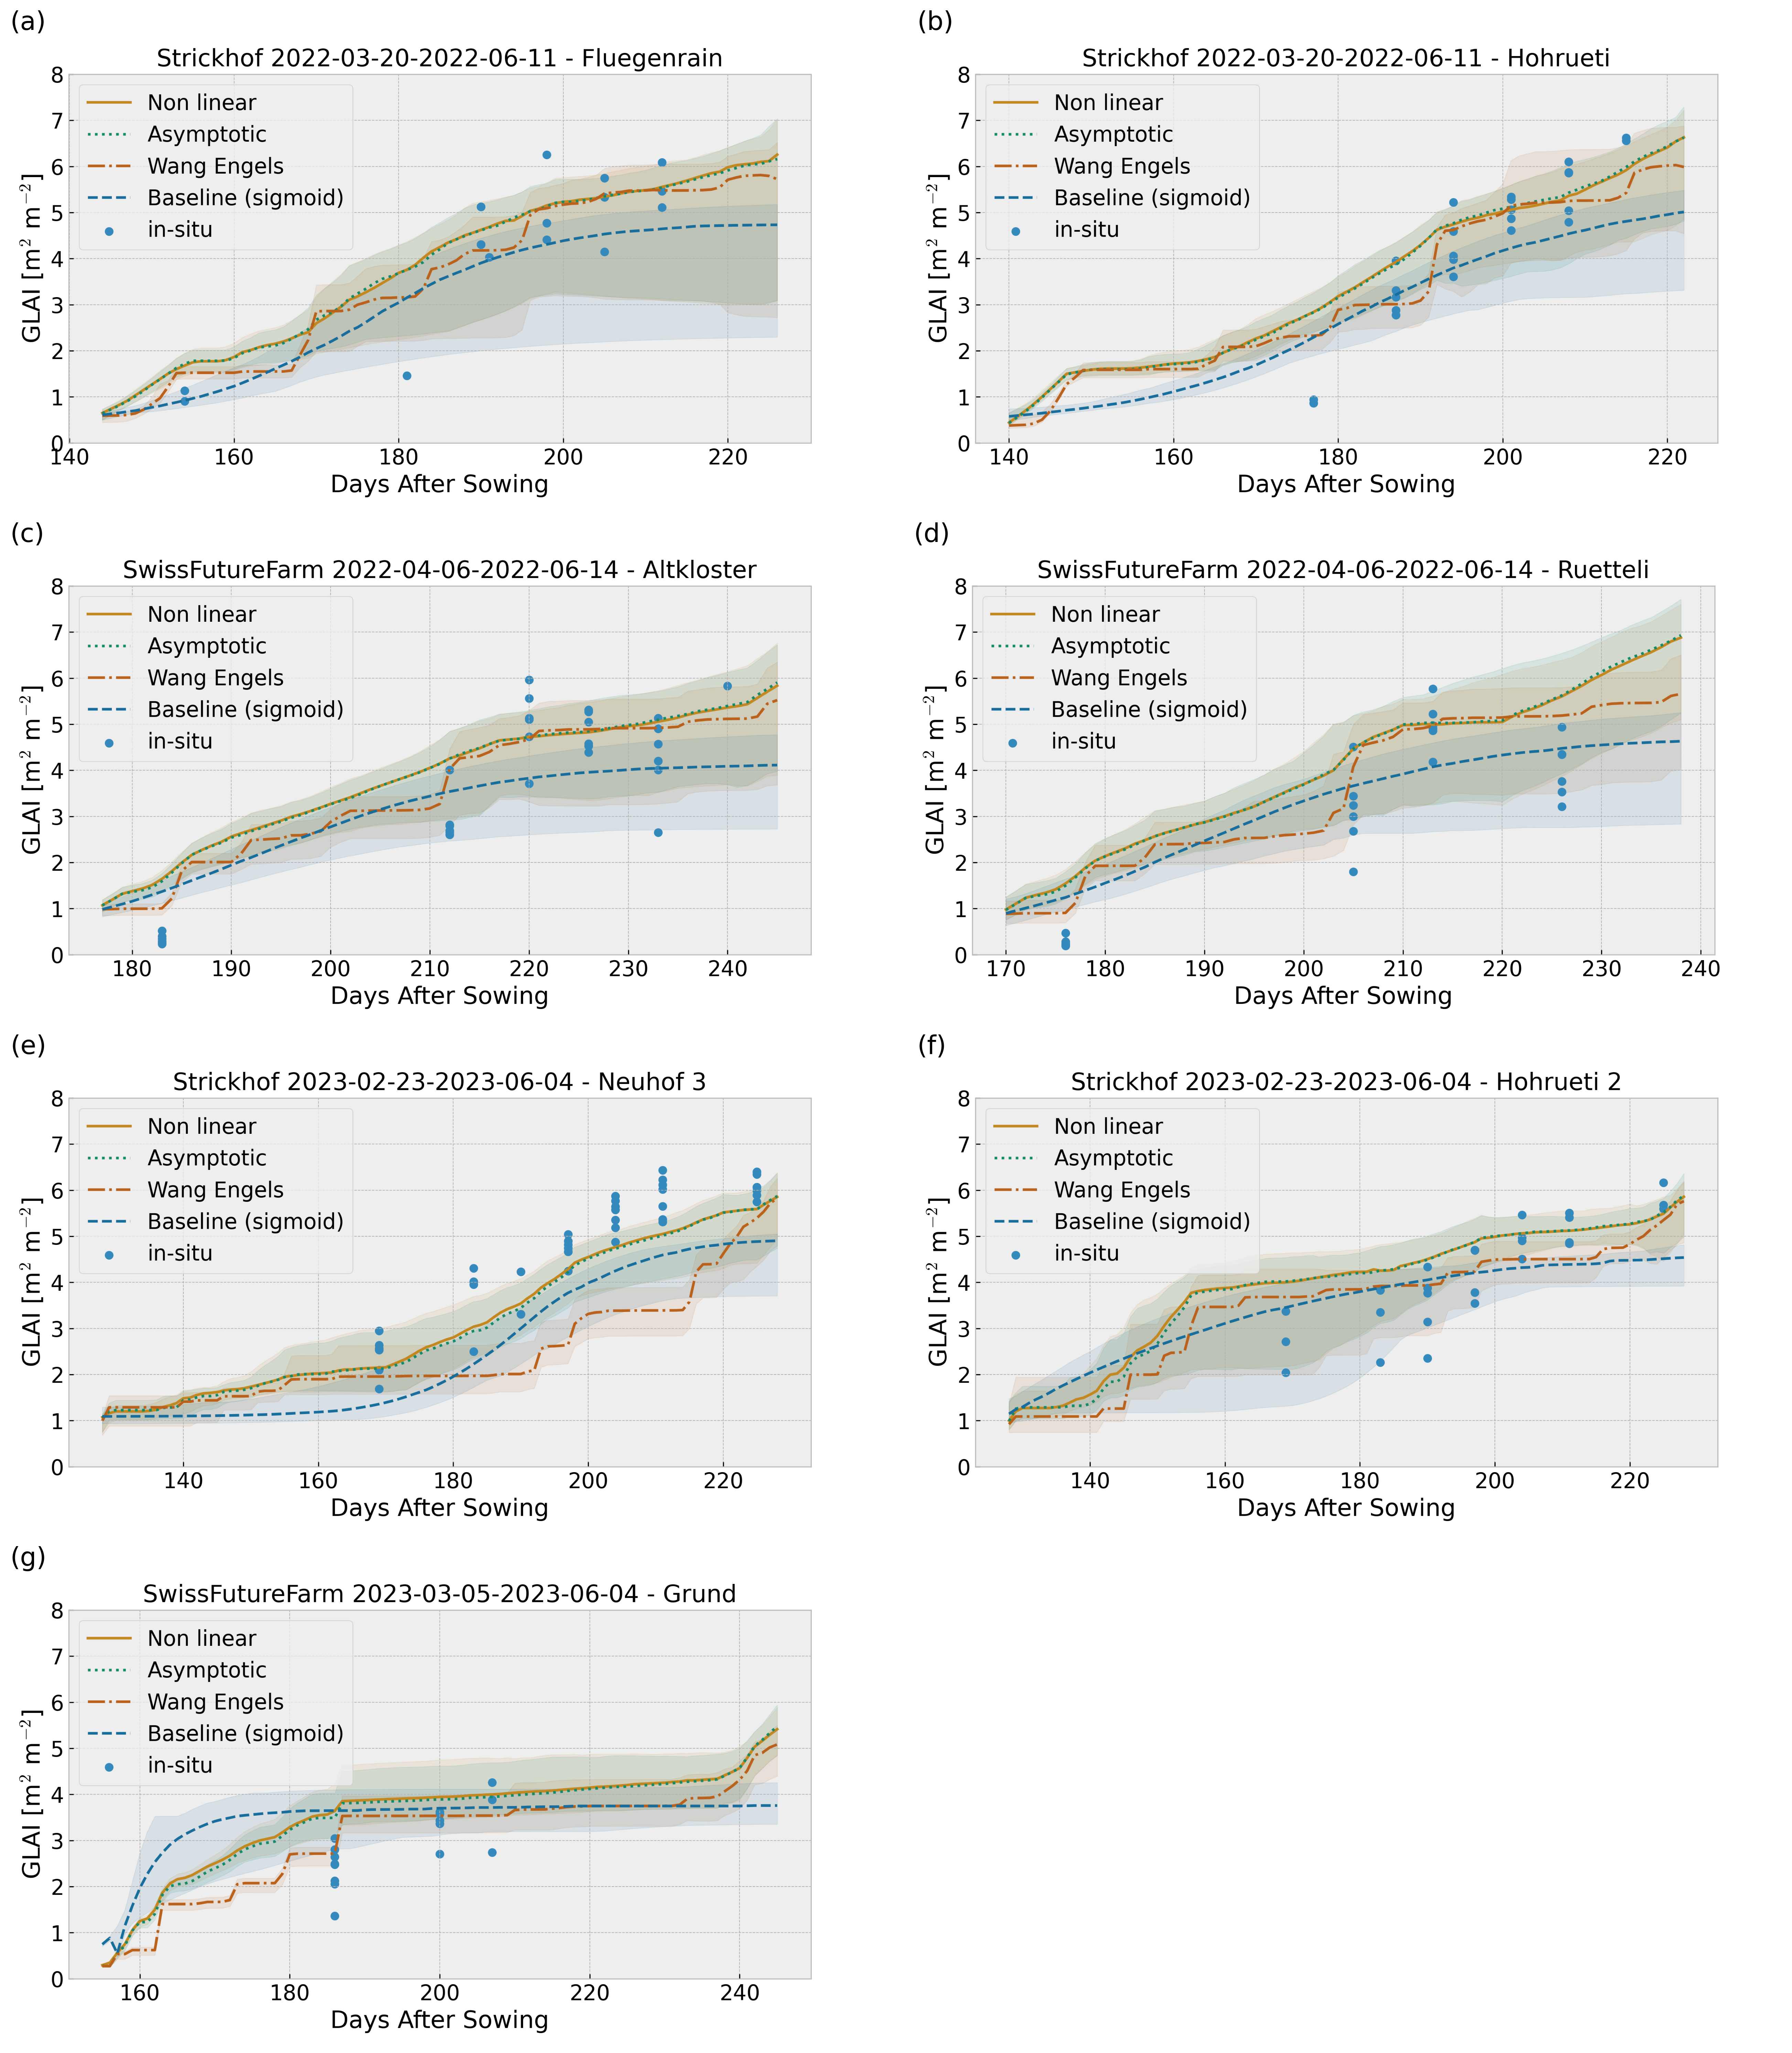
\includegraphics[width=\textwidth]{glai_daily-temporal_profiles.png}
    \caption{Median daily reconstructed \gls{DRC} and baseline \gls{GLAI} time series (lines) and spatial in-field variability in terms of the 5\% to 95\% percentile spread (filled areas) at the field parcels of the validation site (Figure~\ref{fig:map-validation-sites}). The in-situ \gls{GLAI} values are denoted as blue dots.}
    \label{fig:glai-trajectories}
\end{figure}

To further highlight the difference between the \gls{DRC} and the baseline \gls{GLAI}, we plotted the daily asymptotic \gls{DRC} \gls{GLAI} which achieved overall high accuracy (see Tables \ref{tab:error-stats}-\ref{tab:error-stats-years}), against the baseline \gls{GLAI} considering all pixels and dates. The resulting scatter plots are shown for each validation site and year in Figure \ref{fig:model-intercomparison}. In Figure \ref{fig:model-intercomparison}a-c it becomes clear that the baseline \gls{GLAI} reconstructed slightly lower \gls{GLAI} values than the asymptotic \gls{DRC}. The effect was particularly pronounced for GLAI values > 5 $m^2$ $m^{-2}$, as shown by the systematic deviation from the 1:1 line. In Figure \ref{fig:model-intercomparison}d the effect is less pronounced. This site (Swiss Future Farm 2023), however, was also affected by a high proportion of pixels that could not be reconstructed in the baseline \gls{GLAI}, as we will show in the next section.

\begin{figure}[H]
    \centering
    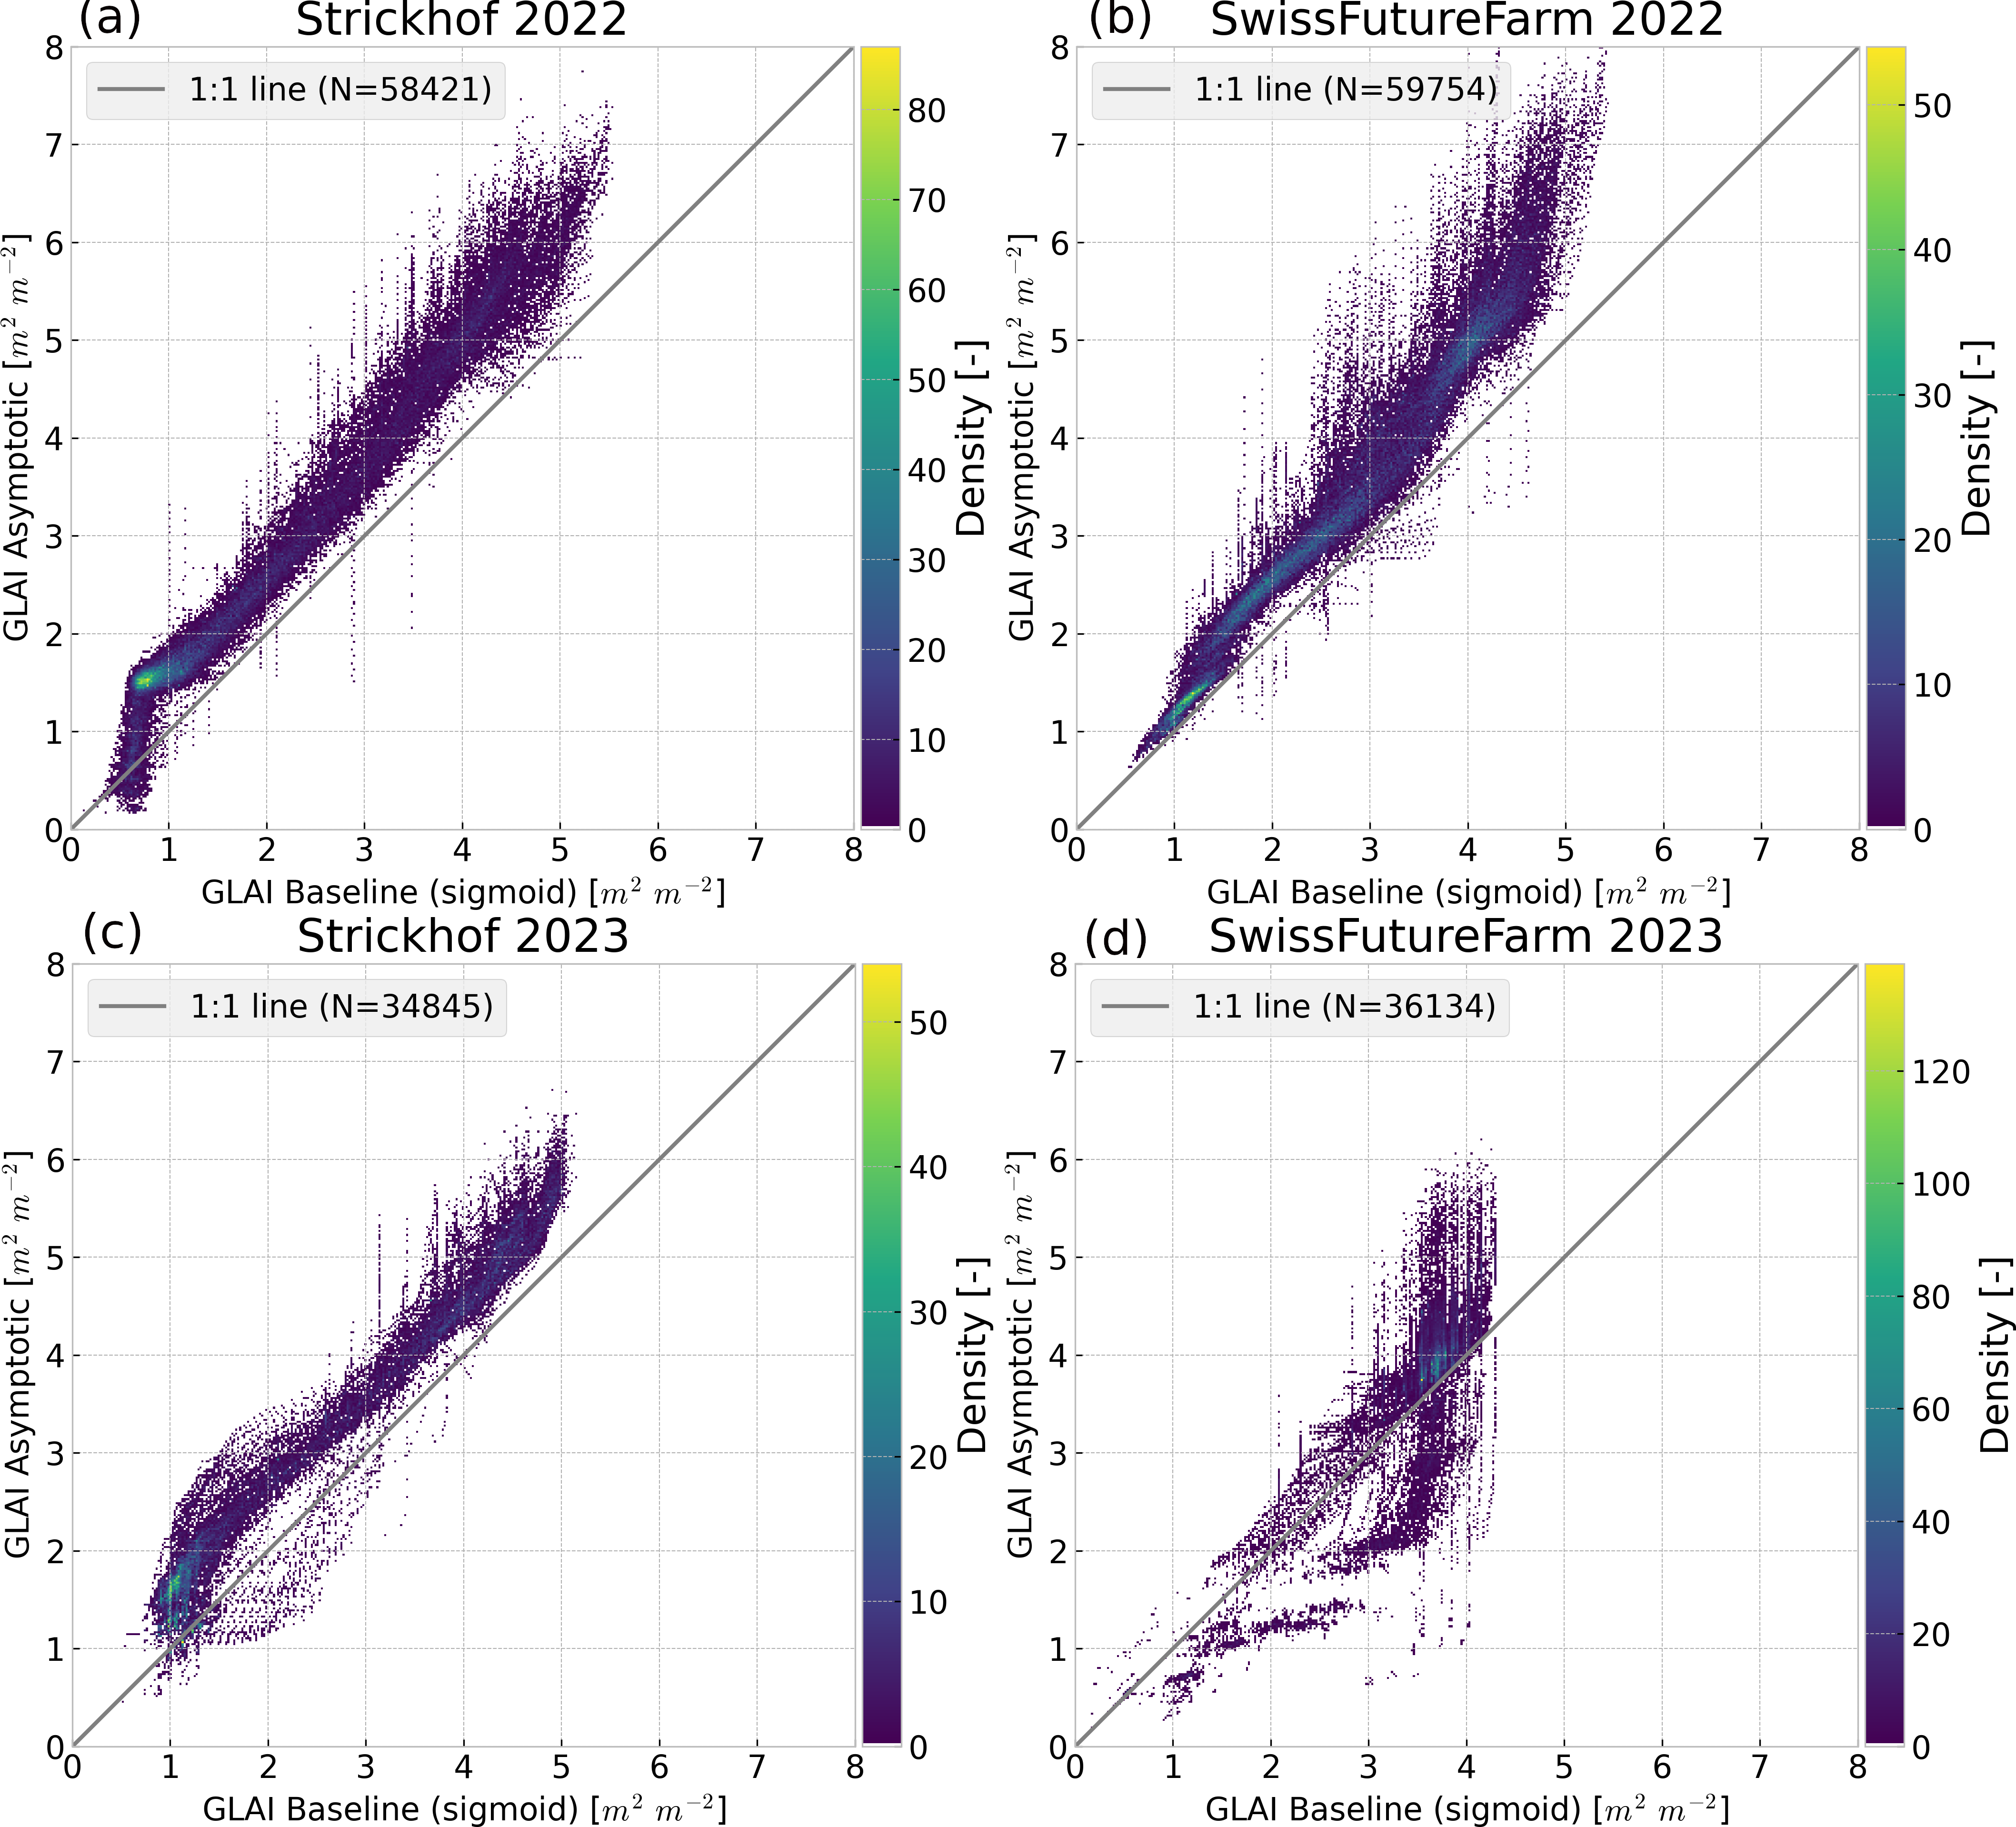
\includegraphics[width=\textwidth]{model_intercomparison_2022-2023.png}
    \caption{Intercomparison of reconstructed GLAI time series values at the Strickhof and Swiss Future Farm sites in 2022 (a, b), and 2023 (c, d), respectively, showing all reconstructed GLAI values from the asymptotic DRC GLAI plotted against all reconstructed baseline GLAI values.}
    \label{fig:model-intercomparison}
\end{figure}


\subsection{GLAI reconstruction success rate}
\label{subsec:glai-reconstruction-sucess}
As described in Section~\ref{subsubsec:baseline-method}, the baseline requires at least four valid raw \gls{S2} \gls{GLAI} values to estimate the function parameters. However, this requirement was not met for all \gls{S2} pixels: While the overall number of \gls{S2} observations is higher than four at all sites (see Section \ref{subsec:s2-imagery}), the \gls{SCL} and simple outlier filtering (Section~\ref{subsubsec:s2-glai-simple-outlier-filter}) caused the total number of valid raw \gls{GLAI} observations to drop below the threshold of four in some cases. Overall, the baseline \gls{GLAI} could not be fitted to 12.43\% of the pixels at the validation sites, with variations from 5.46\% at the Swiss Future Farm in 2022 to 20.08\% at the same site in 2023. The latter case is displayed in Figure \ref{fig:maps-baseline-failure} comparing the daily asymptotic \gls{DRC} \gls{GLAI} to baseline \gls{GLAI} for two dates during late stem elongation and heading. The failure of the baseline to reconstruct \gls{GLAI} values was caused in two thirds of the pixels by a too low number of valid raw \gls{GLAI} observations (< 4), and in one third by the non-convergence of the optimization algorithm after reaching the maximum number of iterations (1000). Although often only pixels at the parcel boundaries were affected, about 40\% of the pixels were located within the parcels, resulting in undesired spatial gaps in the reconstructed baseline \gls{GLAI} (c.f., Figure \ref{fig:maps-baseline-failure}, right). In contrast, for the \gls{DRC} \gls{GLAI}, which only require a minimum number of two valid \gls{GLAI} observations, reconstruction could be performed for all \gls{S2} pixels.

\begin{figure}[H]
    \centering
    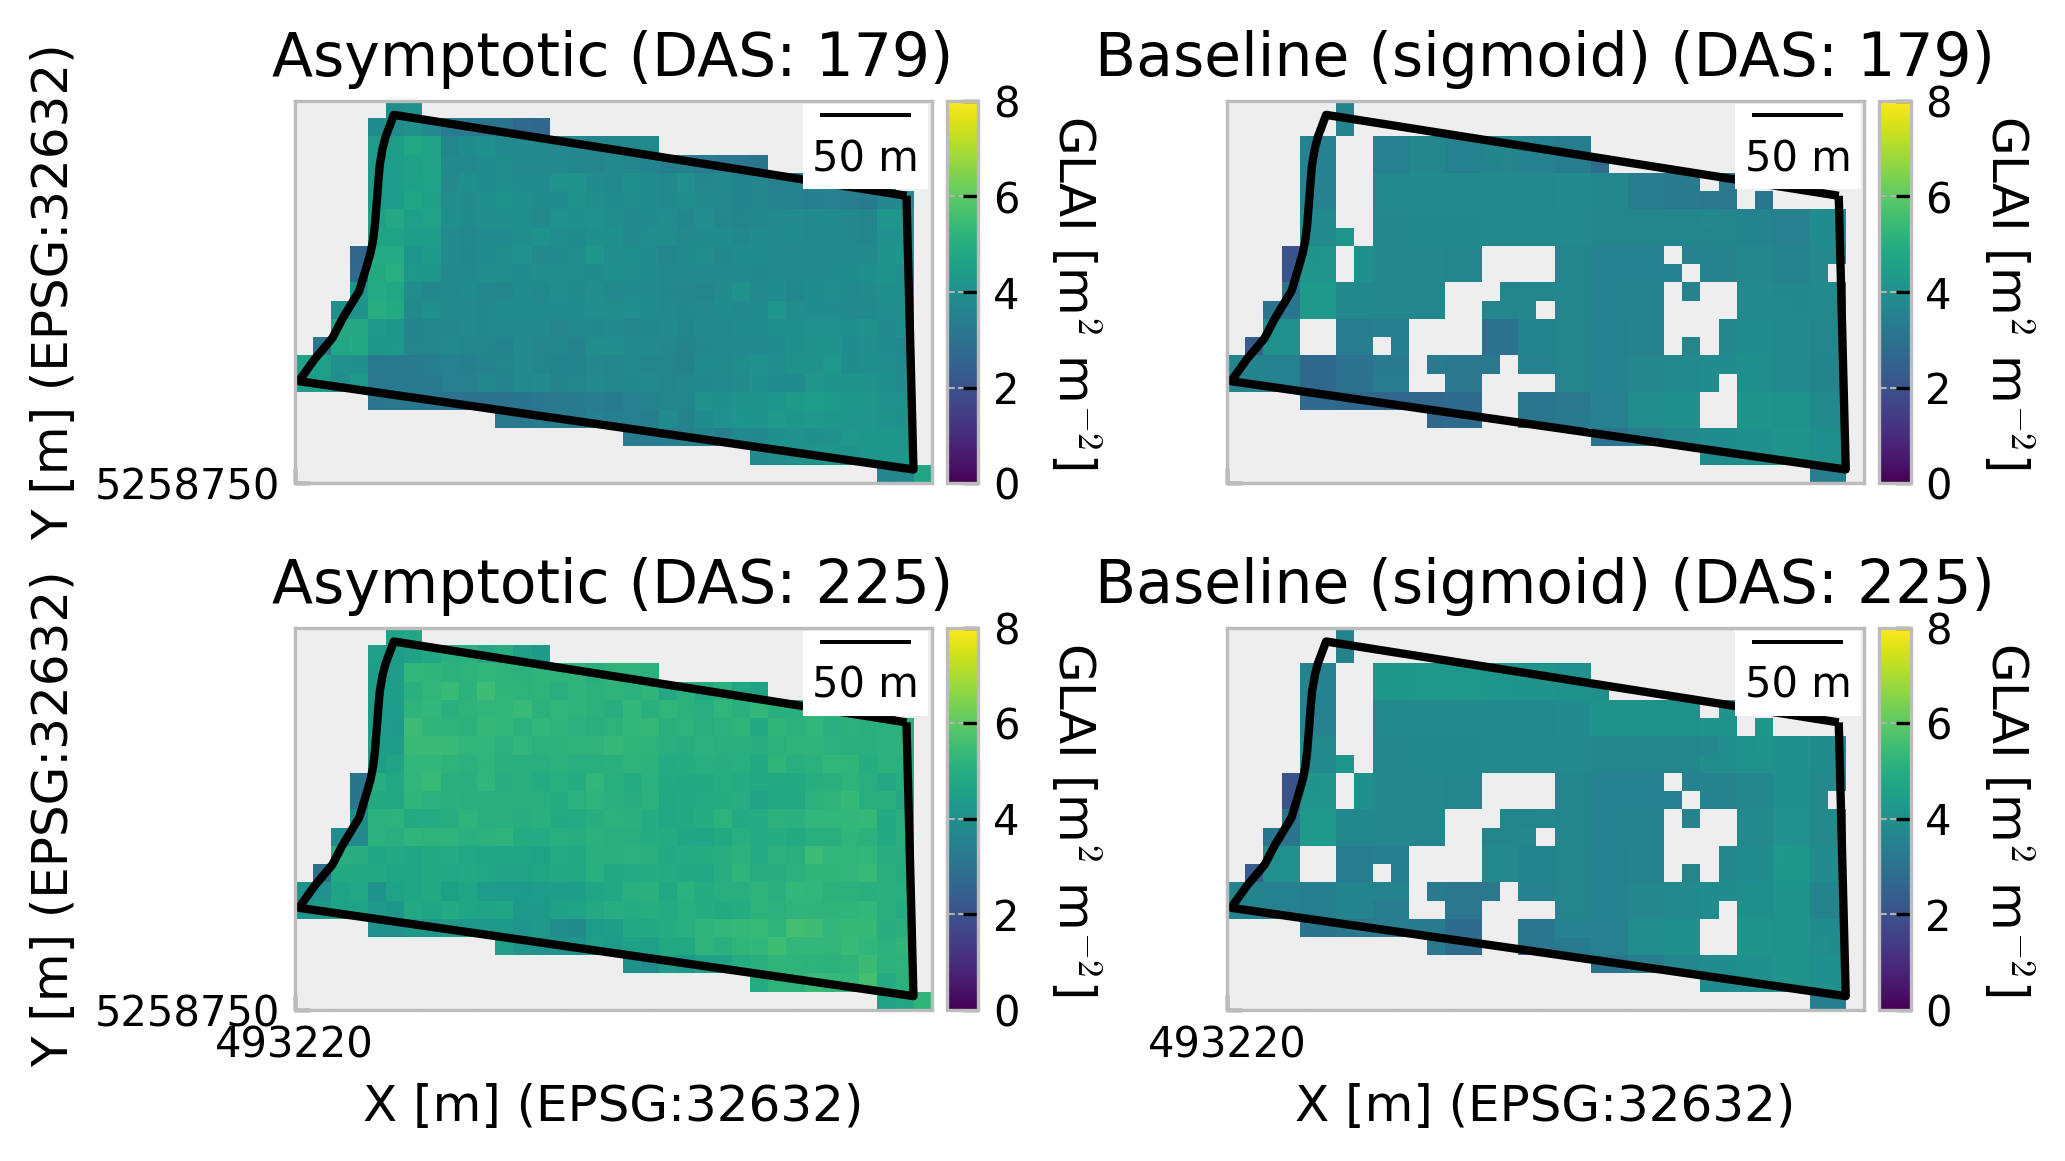
\includegraphics[width=\textwidth]{SwissFutureFarm_2023_Grund_asymptotic-sigmoid.png}
    \caption{Maps of daily asymptotic DRC (left) and baseline GLAI (right) for the parcel Grund at Swiss Future Farm in 2023 for two dates during late stem elongation (top) and heading (bottom) expressed as days after sowing (DAS). The parcel boundary is shown as black line.}
    \label{fig:maps-baseline-failure}
\end{figure}
\subsection{Phenological macro stages}
\label{subsec:res-pheno-macro stages}

From a total of 970 S2 observations over the sampling points (Table \ref{tab:site_characteristics}), 134 (14\%) were located in the AGDD windows determined from phenotyping (Table \ref{tab:bbch-agdd}). The number is based on the requirement that a S2 observation must be within $\pm$20 AGDD to an in-situ observation. In the GE-ET to SE-EH transition window 23 out of 80 S2 observations could be compared to in-situ BBCH ratings. In the second window (SE-EH to FL-PM) it was 8 out of 54 observations.

The purely temperature-based AGDD-PHENO scenario predicted nearly all three stages correctly resulting in an adjusted, i.e., multi-class, F1-score of 0.96. In detail, the class-specific F1-score for GE-ET was 0.93, 0.95 for SE-EH and 1.0 for FL-PM. The confusion matrix is shown in Table \ref{tab:bbch-conf-matrix_agdd-pheno} comparing in-situ rated macro stages to model predictions. Six out of 42 observations (14\%) were wrongly assigned to the SE-EH stage by the model as can been in the confusion matrix (Table \ref{tab:bbch-conf-matrix_agdd-pheno}). For the second transition all data points were assigned to the correct phenological macro stage.

\begin{table}[H]
    \centering
    \caption{Confusion matrix showing in-situ rated and AGDD-PHENO predicted phenological macro stages for sampling dates in 2022 with S2 imagery available (N=148).}
    \label{tab:bbch-conf-matrix_agdd-pheno}
    \begin{tabular}{cc|c|c|c|}
    &\multicolumn{1}{c}{}&\multicolumn{3}{c}{\textbf{AGDD-PHENO Predicted}}\\
    &\multicolumn{1}{c}{}&\multicolumn{1}{c}{\textbf{GE - ET}}
    &\multicolumn{1}{c}{\textbf{SE - EH}}
    &\multicolumn{1}{c}{\textbf{FL - PM}}\\
    \cline{3-5}
    \multicolumn{1}{c}{\multirow{3}{*}{\rotatebox{90}{\textbf{In-Situ Rated}}}}
    &\textbf{GE - ET} &42 & 6 &0 \\
    \cline{3-5}
    &\textbf{SE - EH} &0 & 61 &0\\
    \cline{3-5}
    &\textbf{FL - PM} &0 & 0 & 39\\
    \cline{3-5}
    \end{tabular}
\end{table}

The performance of the AGDD-S2-PHENO scenario was slightly lower as shown in the confusion matrix in Table \ref{tab:bbch-conf-matrix}. This was due to an additional confusion in the second transition window of three observations. Still, the adjusted, i.e., multi-class, F1-score of the AGDD-S2-PHENO model was 0.94 as most observations were assigned correctly based on AGDDs. For the single phenological stages, the F1-score was 0.93, 0.93, and 0.96, for GE-ET, SE-EH, and FL-PM, respectively.

\begin{table}[H]
    \centering
    \caption{Confusion matrix showing in-situ rated and AGDD-S2-PHENO predicted phenological macro stages for sampling dates in 2022 with S2 imagery available (N=148).}
    \label{tab:bbch-conf-matrix}
    \begin{tabular}{cc|c|c|c|}
    &\multicolumn{1}{c}{}&\multicolumn{3}{c}{\textbf{AGDD-S2-PHENO Predicted}}\\
    &\multicolumn{1}{c}{}&\multicolumn{1}{c}{\textbf{GE - ET}}
    &\multicolumn{1}{c}{\textbf{SE - EH}}
    &\multicolumn{1}{c}{\textbf{FL - PM}}\\
    \cline{3-5}
    \multicolumn{1}{c}{\multirow{3}{*}{\rotatebox{90}{\textbf{In-Situ Rated}}}}
    &\textbf{GE - ET} &42 & 6 &0 \\
    \cline{3-5}
    &\textbf{SE - EH} &0 & 61 &0\\
    \cline{3-5}
    &\textbf{FL - PM} &0 & 3 & 36\\
    \cline{3-5}
    \end{tabular}
\end{table}

\subsection{Functional Trait Retrieval}
\label{subsec:res-trait-retrieval}
\subsubsection{Green Leaf Area Index}

The accuracy of GLAI prediction increases by adding phenological priors. Figure \ref{fig:glai-val-scatter} shows scatter plots of in-situ measured GLAI on the x-axis and GLAI from PROSAIL inversion on the y-axis for the three scenario setups. In the baseline scenario without phenology (NO-PHENO), the RMSE is 1.15 $m^2$ $m^{-2}$ (nRMSE: 42.30\%) and the NMAD is 0.77 $m^2$ $m^{-2}$. The scenarios with phenology have lower errors, with the AGDD-PHENO scenario achieving slightly higher accuracy with an RMSE of 0.85 $m^2$ $m^{-2}$  (nRMSE 31.25\%, NMAD 0.09 $m^2$ $m^{-2}$ ) than AGDD-S2-PHENO, where the RMSE is 0.87 $m^2$ $m^{-2}$ (nRMSE 31.89\%, NMAD 0.08 $m^2$ $m^{-2}$ ). In all three cases, modeled GLAI was able to explain between 77 (NO-PHENO) and 84\% (AGDD-PHENO and AGDD-S2-PHENO) of the variance in the in-situ data.

The higher overall accuracy is mainly due to the first phenological phase (GE-ET), in which the RMSE decreases from 0.6 $m^2$ $m^{-2}$ (nRMSE 217.52\%) in the case of NO-PHENO to 0.16 $m^2$ $m^{-2}$ (nRMSE: 58.04\%) in the AGDD-PHENO setup (N=42). We assume the increase in retrieval accuracy was mainly due to optimization in the inversion setup (see Table \ref{tab:inv-setup}): When using a larger LUT and a higher number of solutions, the retrieval error increased to > 100\%. The ill-posedness of RTM inversion, however, makes it difficult to make a conclusive statement. Without optimizing the inversion setup, the retrieval error was up 100\%. In the SE-EH macro stage, the NO-PHENO scenario is slightly better than the AGDD-PHENO scenario with an RMSE of 0.88 $m^2$ $m^{-2}$ and 0.95 $m^2$ $m^{-2}$, respectively (relative errors: 22.08\% and 23.75\%, N=67). In the last phenological macro stage, both models performed similar with an RMSE of 1.07 $m^2$ $m^{-2}$ (relative error: 23.1\%, N=39). In these two stages, the RTM inversion setup was the same for both approaches as suggested by the systematic optimization approach.

\begin{figure}[H]
    \centering
    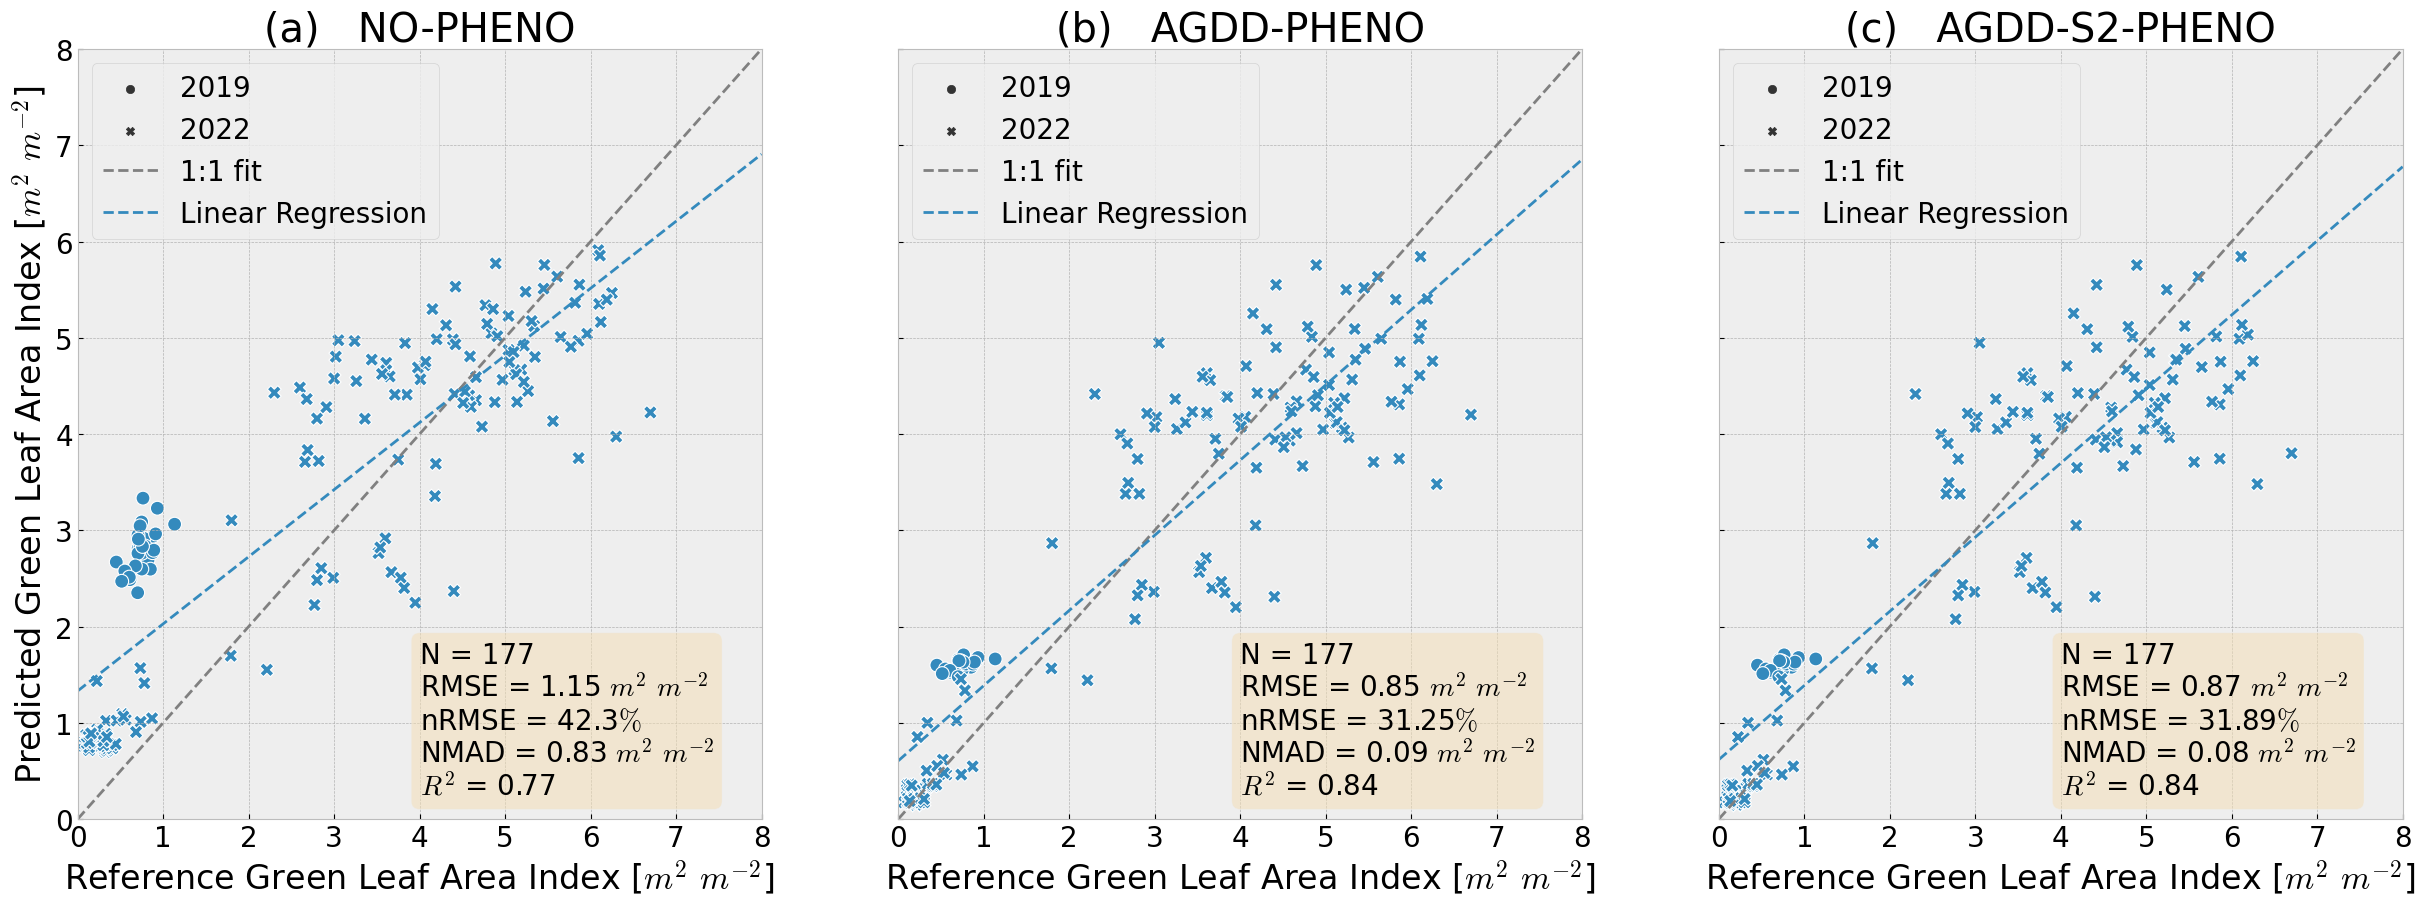
\includegraphics[width=1.0\textwidth]{lai_scatter_plot.png}
    \caption[Scatter plots between in-situ reference and RTM-derived GLAI for the NO-PHENO (a), AGDD-PHENO (b), and AGDD-S2-PHENO (c) scenarios. The year the data was collected is denoted by dots (2019) and crosses (2022).]{Scatter plots between in-situ reference and RTM-derived GLAI for the NO-PHENO (a), AGDD-PHENO (b), and AGDD-S2-PHENO (c) scenarios. The year the data was collected is denoted by dots (2019) and crosses (2022).}
    \label{fig:glai-val-scatter}
\end{figure}

\subsubsection{Canopy Chlorophyll Content}

As with GLAI, the incorporation of phenology shows an increase in the accuracy of CCC retrieval. Unfortunately, fewer data points (N=59) are available for validation of CCC. Also, these are limited to the early growth stages (GE-ET and SE-EH). Figure \ref{fig:ccc-val-scatter} shows the in-situ measured versus modeled CCC. The RMSE of CCC retrieval is about 0.37 $g$ $m^2$ (nRMSE: 55.52\%, NMAD: 0.28 $gm^2$) in the two phenological setups versus an RMSE of 0.66 $g$ $m^2$ (nRMSE 98.62\%, NMAD: 0.86 $g$ $m^2$) in the NO-PHENO baseline. The modeled CCC explained between 79 and 84\% of the variance in the in situ values. When looking at the 2019 data alone (N=29, see cross markers in Figure \ref{fig:ccc-val-scatter}), an extremely poor retrieval performance can be observed with an $R^2$ of around 0.02. AGDD-PHENO and AGDD-S2-PHENO (Figure \ref{fig:ccc-val-scatter}b, c) show the same retrieval accuracy as the data only includes data points for which both models agreed on the same phenological macro stage.

\begin{figure}[H]
    \centering
    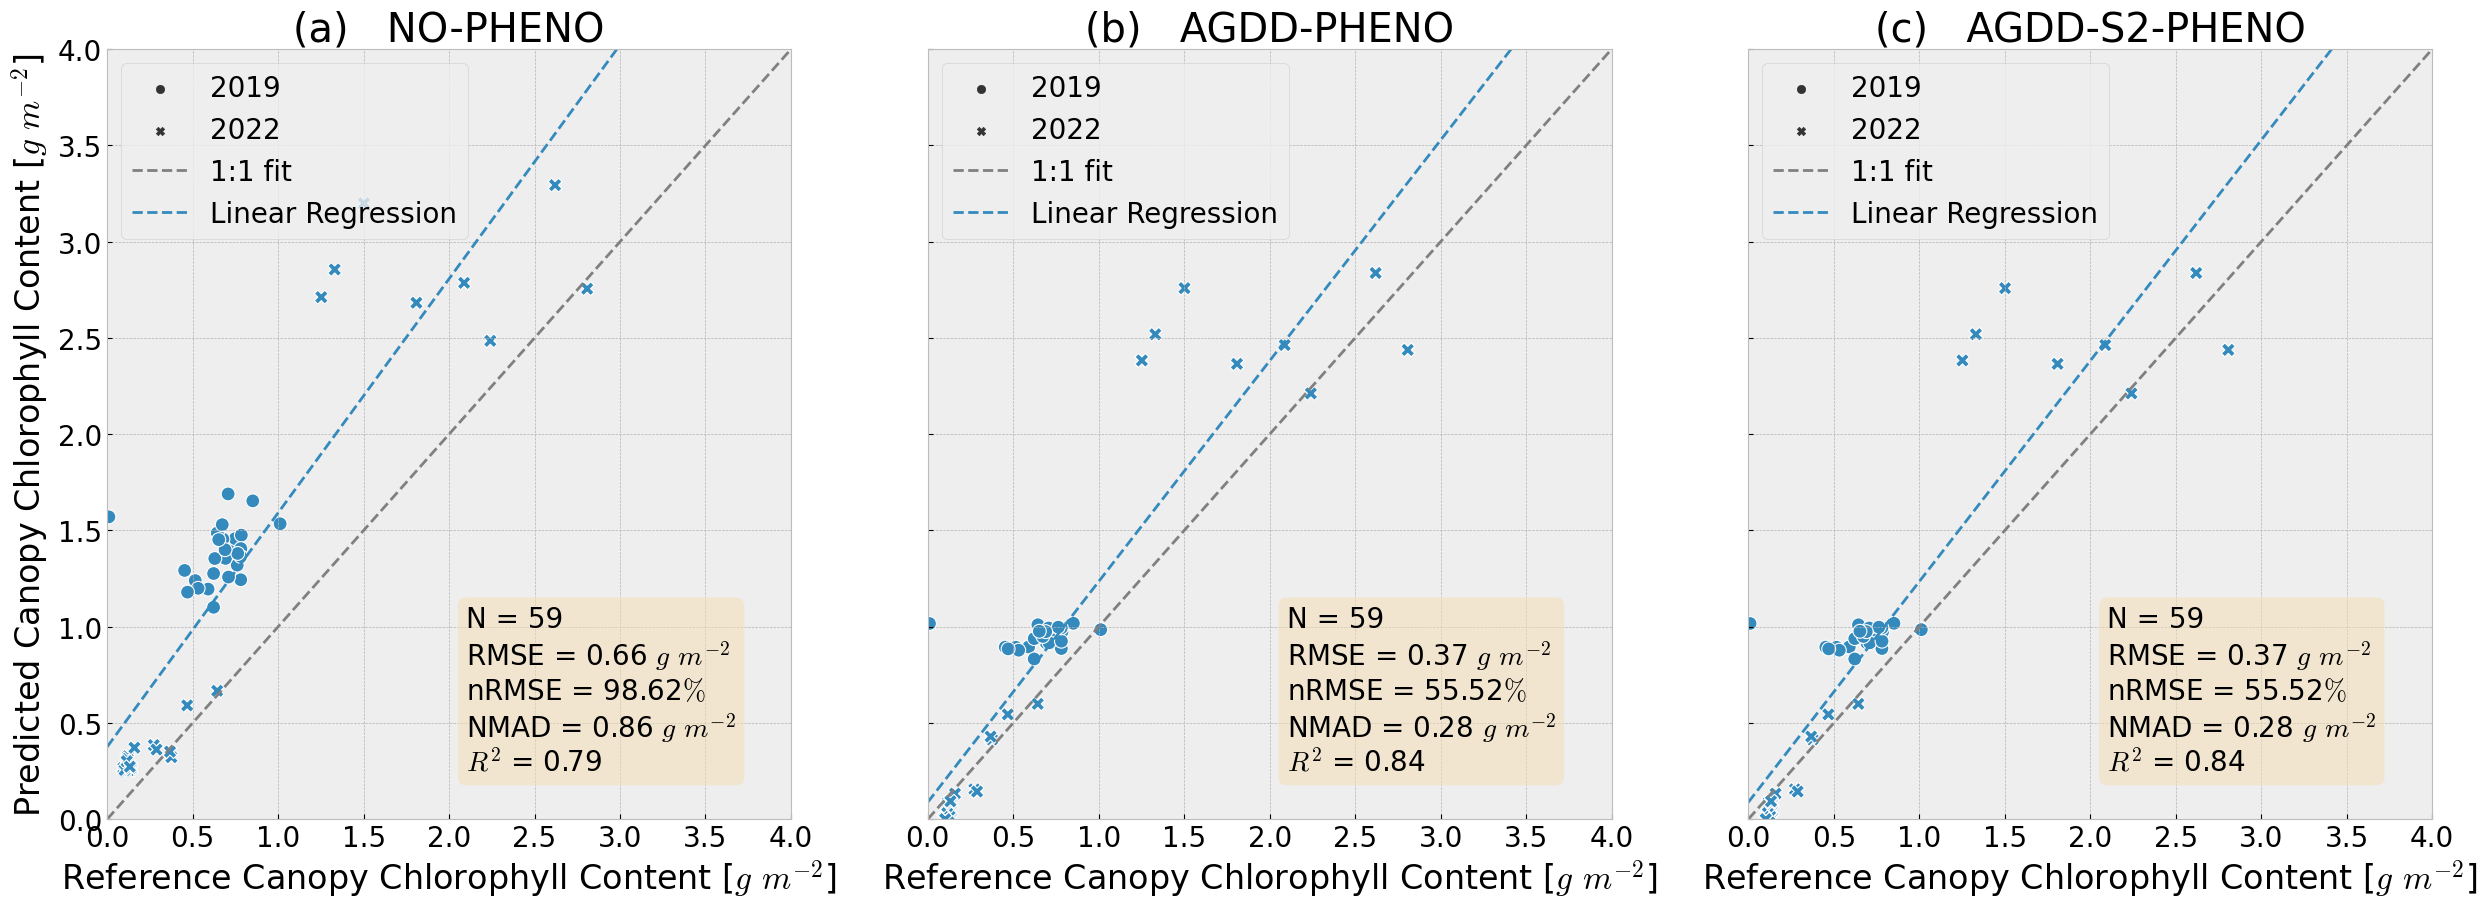
\includegraphics[width=1.0\textwidth]{ccc_scatter_plot.png}
    \caption[Scatter plots between in-situ reference and RTM-derived CCC for the NO-PHENO (a), AGDD-PHENO (b), and AGDD-S2-PHENO (c) scenario setups. The year the data was collected is denoted by dots (2019) and crosses (2022).]{Scatter plots between in-situ reference and RTM-derived CCC for the NO-PHENO (a), AGDD-PHENO (b), and AGDD-S2-PHENO (c) scenario setups. The year the data was collected is denoted by dots (2019) and crosses (2022).}
    \label{fig:ccc-val-scatter}
\end{figure}


\subsubsection{Spatio-Temporal Considerations}

Figure \ref{fig:trait-maps-wtz} shows maps of modeled GLAI (top row), CCC (middle row), and Cab (bottom row) for selected S2 scenes in 2022 for the Witzwil site (Parzelle 35) depicting all three phenological macro stages. Traits are based on the AGDD-PHENO scenario which outperformed the other two setups in terms of trait retrieval accuracy. Figure \ref{fig:trait-maps-wtz} shows the high correlation between GLAI and CCC when comparing them on a pixel-by-pixel basis ($R^2$ between 0.97 and 0.99, N=2604 pixels per S2 scene). The correlation between GLAI and Cab is more variable and shows a change over the season: for example, $R^2$ is 0.5 at the beginning of stem elongation (20220325, second column from left in Figure \ref{fig:trait-maps-wtz}) and increases to 0.91 at the last date shown (20220618, right column in Figure \ref{fig:trait-maps-wtz}). An increase of trait values starting in March (GE-ET) towards a maximum in May (FL-PM) can be observed (second column from the right in Figure \ref{fig:trait-maps-wtz}) followed by a decrease in the last S2 scene (right column in Figure \ref{fig:trait-maps-wtz}) at the onset of senescence. A clear spatial pattern is visible in the field (upper central part), which can be explained by soil subsidence and associated water logging~\citep{egli_landschaftsdynamik_2020}. The observed field heterogeneity coincides with the experience of the local farmer. The spatial patterns are similar in all three traits.

Maps for the other field parcels studied in 2022 showing the same calendar dates can be found in the Appendix (Figures \ref{fig:appendix_arb_broatefaeld_2022} - \ref{fig:appendix_sff_ruetteli_2022}). Moreover, a map of GLAI, CCC, and Cab for April 20th, 2019 is shown in Figure \ref{fig:appendix_sff_2019} for the two field parcels at which different nitrogen treatments were applied (see Section \ref{subsec:on-farm-trials}).

The high correlation between modeled GLAI and CCC applies to all field parcels and S2 scenes in 2022. The correlation between GLAI and Cab is weaker overall. It shows a seasonal change from low correlation in tillering and beginning of stem elongation to high correlation after ear swelling (BBCH macro stage 40). In 2019, the aforementioned poor retrieval accuracy in GLAI and CCC resulted in lower correlation between modeled GLAI and CCC ($R^2$ around 0.73). This is lower than in the independent calibration dataset (see Section \ref{subsec:model-calibration} and Figure \ref{fig:lai-ccc-relationship}).

\begin{figure}[H]
    \centering
    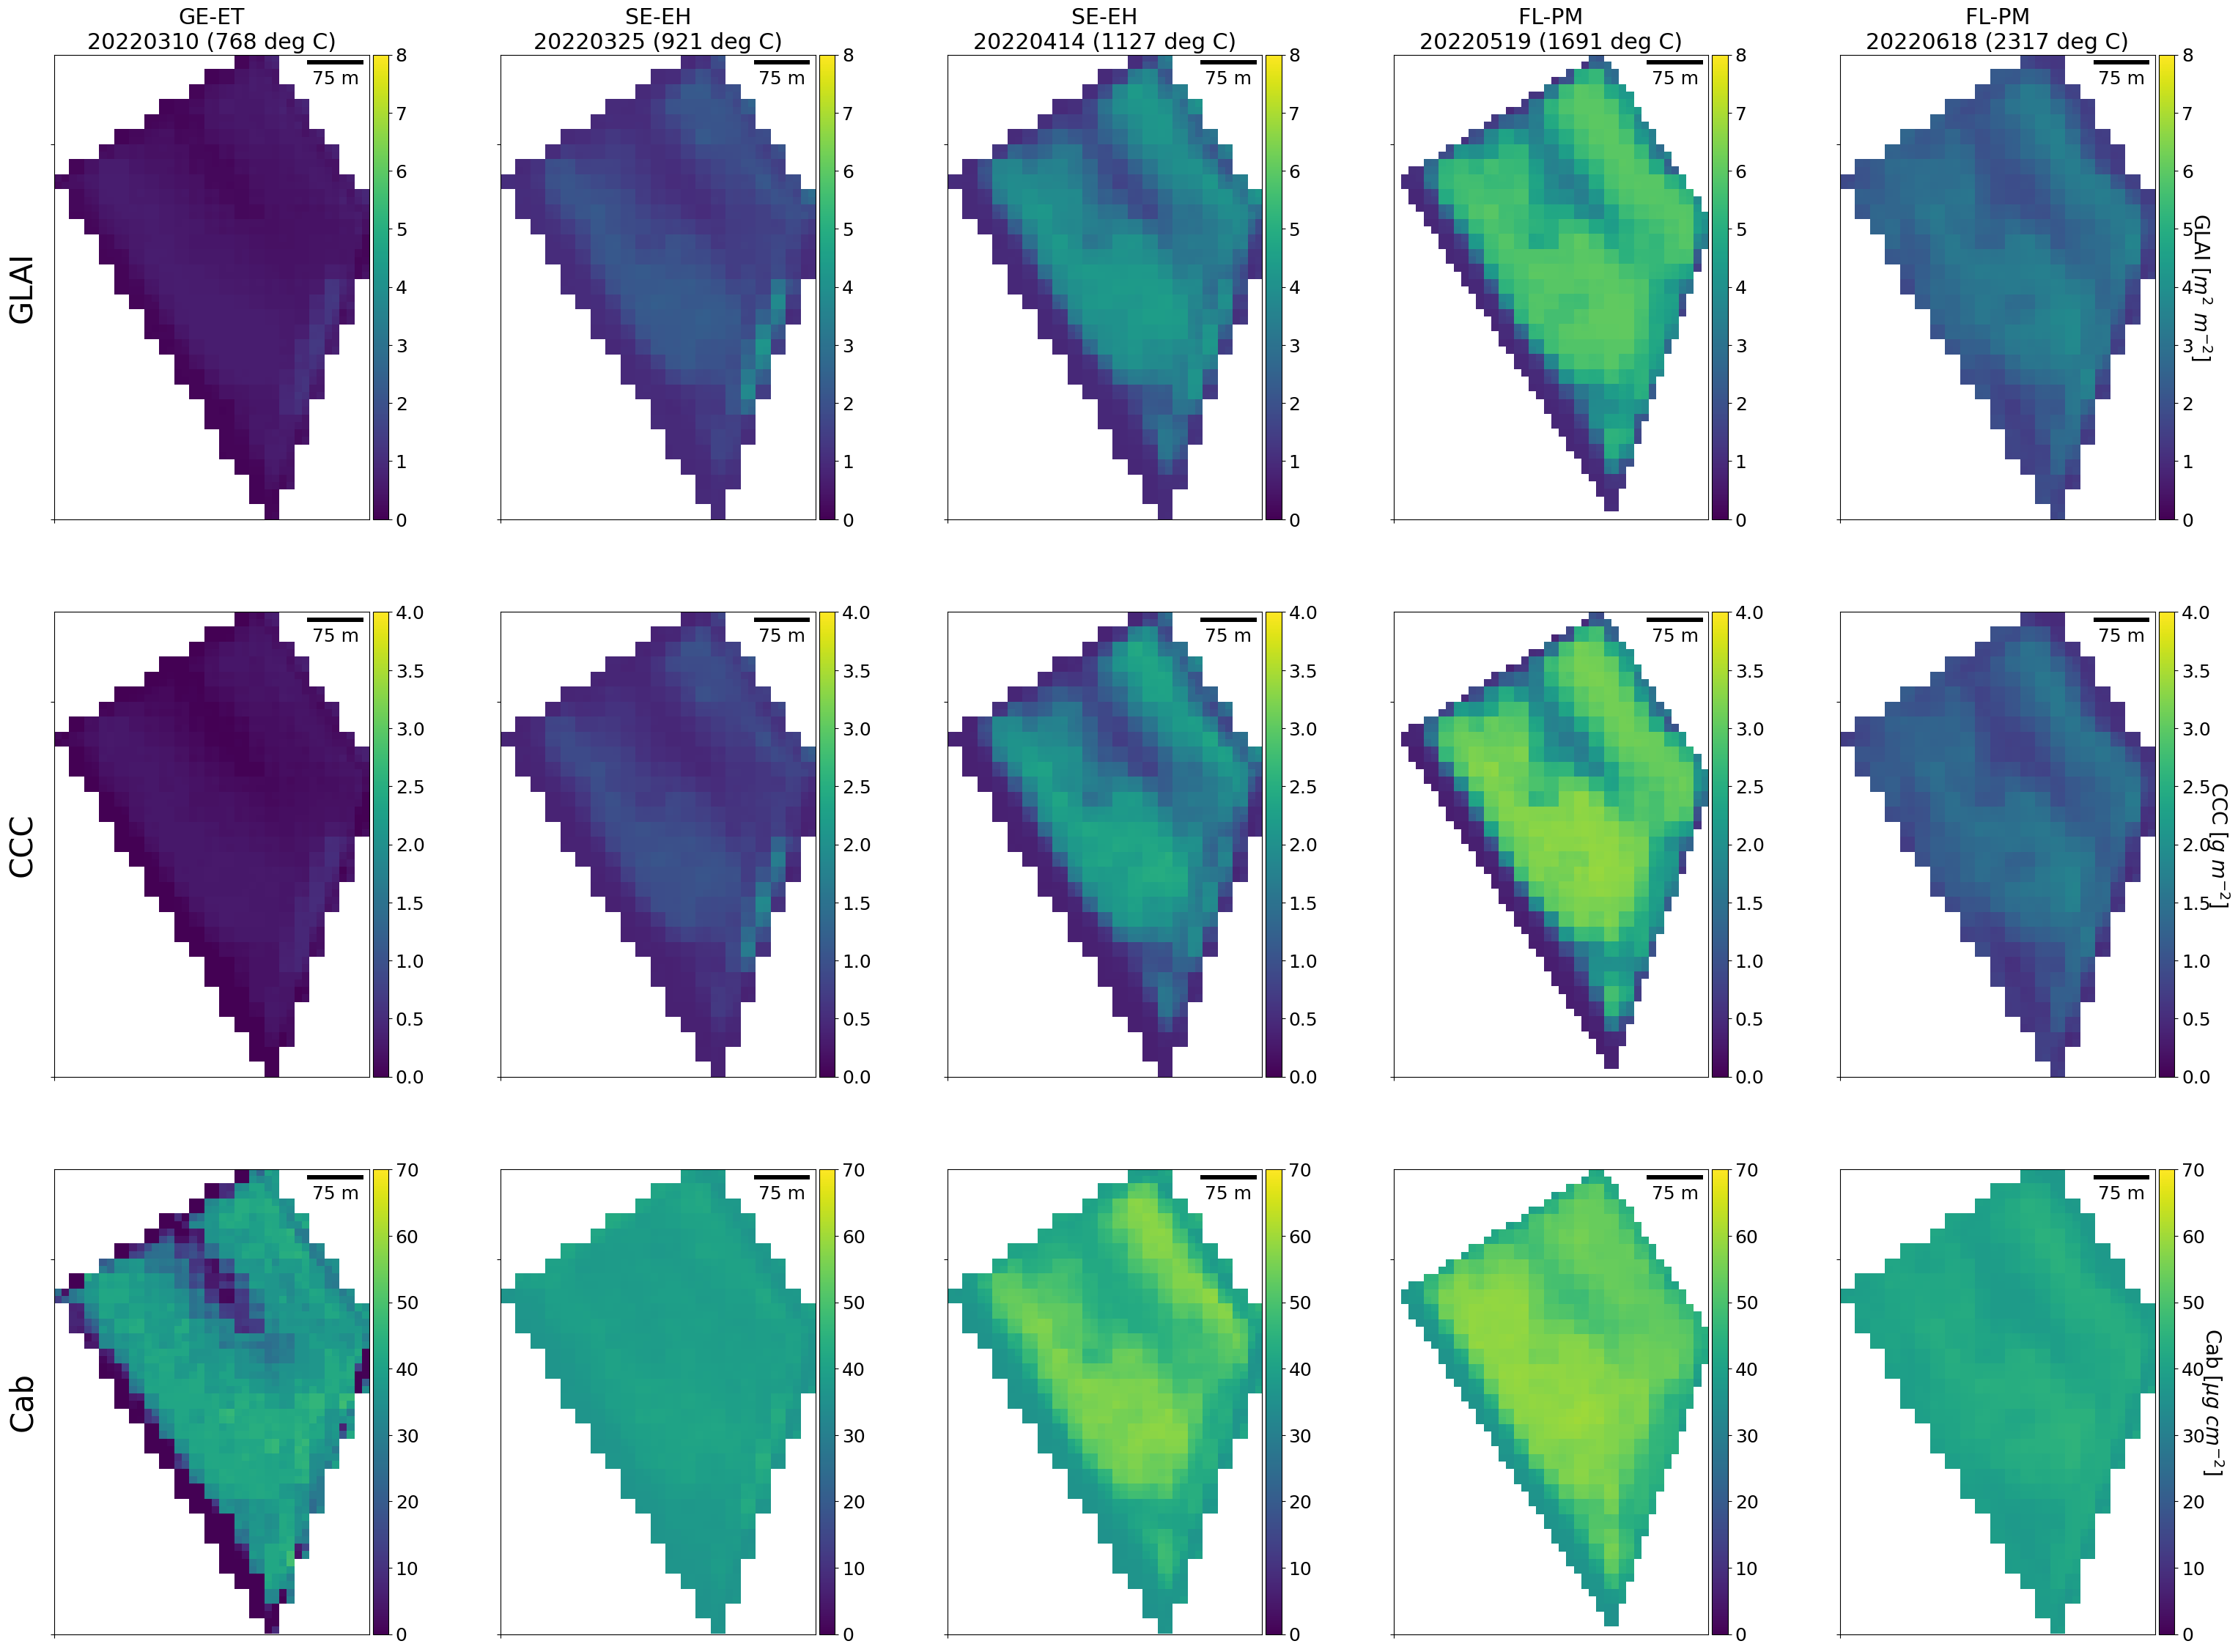
\includegraphics[width=1.0\textwidth]{WTZ_Trait_Maps.png}
    \caption[Maps of GLAI (top), CCC (middle), and Cab (bottom) derived from the best performing scenario (PHENO-AGDD) for Witzil (Parzelle 35). The maps are obtained from selected S2 overpasses depicting the three phenological macro stages of winter wheat (AGDD in brackets).]{Maps of GLAI (top), CCC (middle), and Cab (bottom) derived from the best performing scenario (PHENO-AGDD) for Witzil (Parzelle 35). The maps are obtained from selected S2 overpasses depicting the three phenological macro stages of winter wheat (AGDD in brackets).}
    \label{fig:trait-maps-wtz}
\end{figure}

Figure \ref{fig:ts-dates-agdds} shows median GLAI (top row), CCC (middle row), and Cab (lower row) trajectories derived from the AGDD-PHENO scenario for all field parcels investigated in 2022. Median trait values are plotted per S2 image acquisition date in calendar dates (Figure \ref{fig:ts-dates-agdds}, a) and AGDD (Figure \ref{fig:ts-dates-agdds}, b). For all fields, the traits follow plausible temporal patterns. GLAI values increase steadily from $<1$ $m^2$ $m^{-2}$ at the beginning of March (GE-ET phase) and reach a maximum in early summer (4 to 5.5 $m^2$ $m^{-2}$), followed by a decline in the FL-PM phase reaching values around 1 $m^2$ $m^{-2}$ in mid and late July. CCC closely follows the seasonal trajectory of GLAI (Figure \ref{fig:ts-dates-agdds}, middle row). Cab (Figure \ref{fig:ts-dates-agdds}, lower row) reveals a slightly different picture: Cab values start to increase earlier than GLAI and show only a slight decline towards the end of the season. This means, the same GLAI value (e.g., 1 $m^2$ $m^{-2}$) at the start and end of the season has different Cab levels: Lower Cab levels (< 40 $\mu g$ $cm^{-2}$) at the beginning of the season (around AGDD 700 to 800 deg C)  and higher Cab levels (>= 40 $\mu g$ $cm^{-2}$) during the last phenological macro stage (FL-PM, around AGDD 2200 to 2500 deg C).

By comparing calendar dates and AGDDs, some interesting observations can be made: The GLAI of the organically managed Broatefaeld plot (Arenenberg site, see Table \ref{tab:site_characteristics}) is lower than the GLAI of the other fields and shows a delayed increase of the GLAI in the AGDD scale. Cab levels, however, are similar to the other parcels. In case of Parzelle 35 (Witzwil site) there is an earlier increase of GLAI with respect to calendar dates. However, in the AGDD scale, it can be seen that the wheat in this field lags behind the other fields except for the aforementioned Broatefaeld parcel and also requires a much higher cumulative temperature sum ($\sim$2700 deg C d) to reach maturity. The other six fields already reach this value around AGDD 2200. Notably, in the calendar view, all fields reach these low GLAI values at almost the same time by mid of July when harvest took place (between July 15th at Broatefaeld and July 27th at Ruetteli, SwissFutureFarm).

\begin{figure}[H]
    \centering
    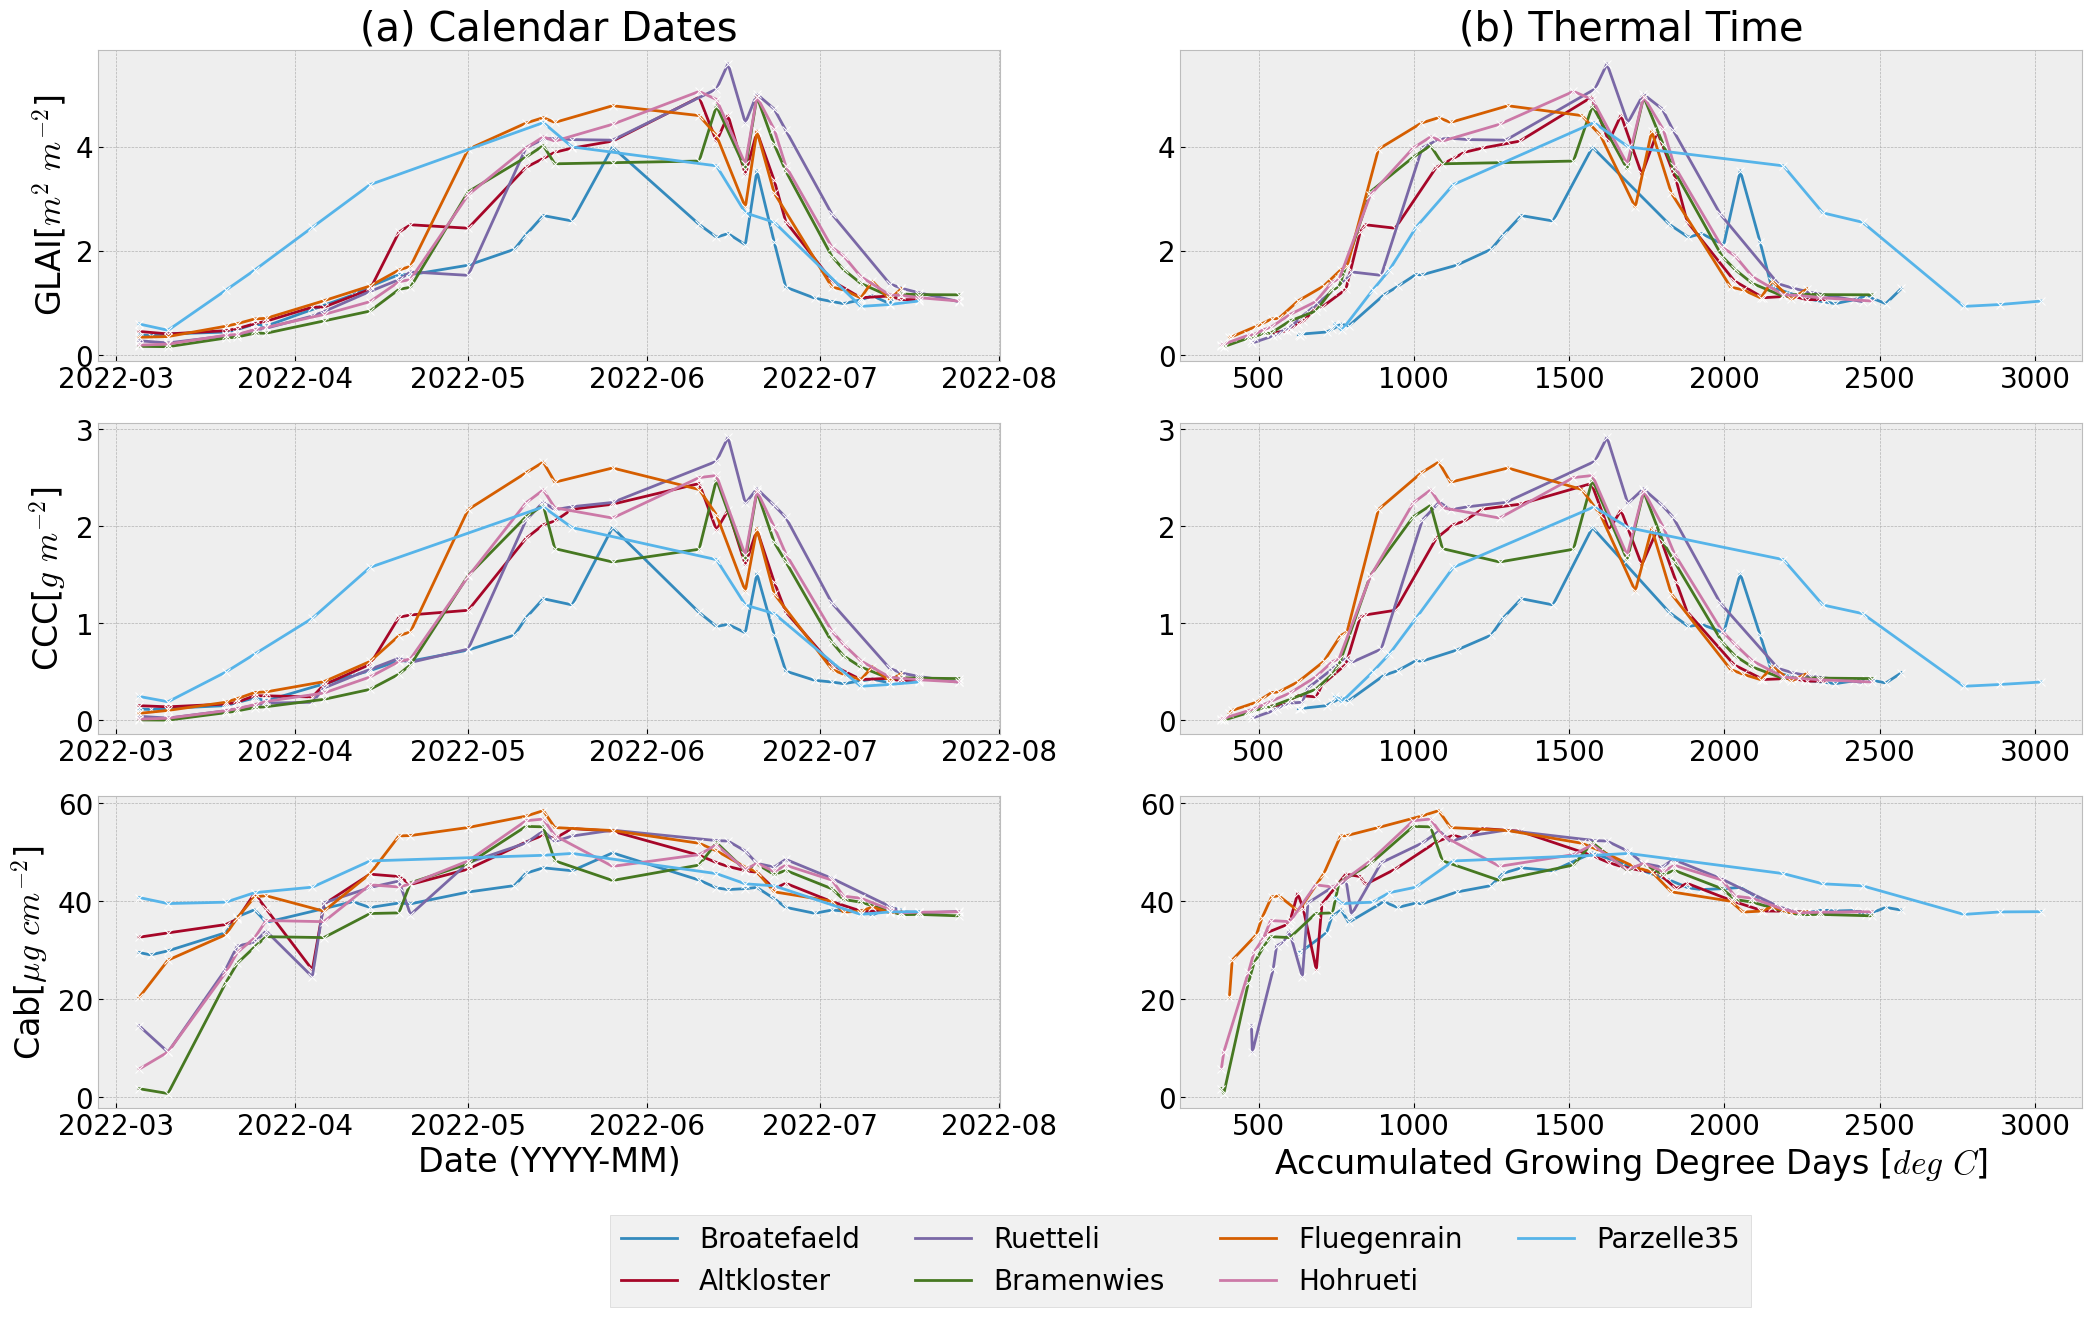
\includegraphics[width=1.0\textwidth]{ts_dates_agdds.png}
    \caption[Trajectories of median GLAI (top row), CCC (middle row), Cab (lower row) values per field parcel with x-axis plotted in calendar dates (a) (i.e., S2 image acquisition dates) and accumulated growing degree days (b).]{Trajectories of median GLAI (top row), CCC (middle row), Cab (lower row) values per field parcel with x-axis plotted in calendar dates (a) (i.e., S2 image acquisition dates) and accumulated growing degree days (b).}
    \label{fig:ts-dates-agdds}
\end{figure}

\section{Discussion}
\label{sec:discussion}
% \subsection{Time series reconstruction accuracy and plausibility}
Although the raw \gls{GLAI} values and the reconstructed \gls{GLAI} are not directly comparable due to the different number of data points, we conclude that the reconstructed \gls{GLAI} values using \gls{DRC}s and the baseline reduced the \gls{GLAI} retrieval error (Figures \ref{fig:s2-obs-scatter-plots} and \ref{fig:glai-scatter-plots}). This was mainly due to the removal of outliers in the negative y-direction caused by atmospheric perturbations, suggesting that both the \gls{DRC} and baseline approaches dealt reasonably well with the effects of undetected clouds and cloud shadows. Nevertheless, a systematic underestimation of GLAI values greater than 5 $m^2$ $m^{-2}$ was observed for the \gls{GLAI} baseline. This underestimation was hardly noticed in the proposed reconstruction with \gls{DRC}s (see Figure \ref{fig:glai-scatter-plots}) as the \gls{DRC} \gls{GLAI} was mostly higher than the baseline (Figures \ref{fig:glai-trajectories} and \ref{fig:model-intercomparison}). The underestimation of \gls{S2} \gls{GLAI} observations was probably due to the \gls{RTM} inversion approach used: It is a known problem that \gls{RTM}s such as PROSAIL exhibit saturation phenomena at high biomass levels due to leaf clumping~\citep{richter_evaluation_2011}. As the baseline only uses the raw \gls{S2} \gls{GLAI} observations, the fit could not compensate for saturation effects, so the reconstructed time series consequently underestimated \gls{GLAI}. In addition, the sigmoid fit aims to minimise the mean error of the reconstructed curve to the raw \gls{S2} \gls{GLAI} observations. This may lead to further underestimation of \gls{GLAI} values, as the reconstructed curve may sometimes be lower than the underlying \gls{S2} \gls{GLAI} observations.

In the case of \gls{DRC}s, the assimilation scheme integrates two data sources with distinct advantages: The \gls{DRC}s contain prior physiological knowledge about the relationship between air temperature and growth, thereby mitigating the underestimation of \gls{GLAI} values as this relationship was established using high-quality in-situ data. The raw \gls{S2} \gls{GLAI} provides spatial details that are absent from the temperature data. This makes the approach well-suited for fine-grained spatial growth analysis. In addition, as air temperature records are usually continuous, the \gls{GLAI} reconstruction between \gls{S2} observations relies on encoded physiological knowledge, reducing the likelihood of unrealistically fast growth rates due to physiological constraints imposed by the temperature. It is not ensured that the baseline will accurately reflect the prevailing conditions. This is due to the fact that reconstruction between \gls{S2} observations solely relies on the function parameters, which do not necessarily contain sufficient information about the underlying biological mechanisms. Consequently, the baseline might indicate high growth rates even if the temperature is significantly below or above the critical $T_{min}$ and $T_{max}$ thresholds.

The accuracy of the \gls{DRC}-reconstructed \gls{GLAI} was comparable to approaches using more complex mechanistic crop growth models, which require a significantly higher number of parameters: \cite{ma_wheat_2022} reported values of $R^2$ between 0.7 and 0.73 for winter wheat in northern China (relative errors between 22 and 26\%) using the SAFYE crop growth model in combination with \gls{S2} images for two growing seasons. This is comparable to the accuracy using \gls{DRC}s (Table \ref{tab:error-stats}). Higher accuracy was reported by \cite{hank_using_2015} for winter wheat in southern Germany. They achieved a root mean square error of 0.35 $m^2$ $m^{-2}$ ($R^2$ 0.96) using a more complex crop growth model combined with Landsat and RapidEye satellite remote sensing data. However, their sample size was small (N = 19) and included only a single growing season and field parcel. Even smaller errors were reported by \cite{zhang_improving_2021} (relative errors between 2.0 and 9.2\%) using SAFYE for two growing seasons of winter wheat in central China. Instead of using satellite imagery, they used \gls{GLAI} retrieved from handheld hyperspectral data, which is arguably not comparable to space-borne \gls{GLAI} retrieval. However, more complex crop growth models often aim to model phenology or even yield, whereas the approach presented is designed to interpolate \gls{GLAI} observations in a physiologically meaningful way. This also means that the reduced complexity, and perhaps accuracy, can be compensated for by using the \gls{GLAI} observations as guidance over the growing season.

However, the \gls{DRC} approach is also likely to be limited by the lack of spatial detail during long periods without \gls{S2} passes due to cloud cover -- a problem shared with more complex crop growth models. Assimilation includes information on crop growth that has causes other than temperature alone, such as differences in soil properties or subtle differences in management. Without regular assimilation, this information cannot be incorporated into the \gls{DRC} growth rates, limiting the accuracy of comparing the reconstructed \gls{GLAI} with in-situ data. Therefore, a higher number of \gls{S2} observations is likely to result in higher reconstruction accuracy. This means that increasing the number of observations, e.g. by fusing \gls{GLAI} from cube satellite constellations as suggested by \cite{sadeh_fusion_2021}, could further increase the reconstruction accuracy. This method has two major drawbacks: First, the amount of data and model complexity increases significantly due to the addition of a second satellite platform. One of the main advantages of the \gls{DRC} approach, however, is its simplicity. Secondly, most cube satellite constellations, unlike \gls{S2}, are commercial products that carry a financial burden that not all users of remote sensing data may be able to bear. Still, as the question of the optimal number of satellite observations and their temporal distribution for data assimilation does not seem to have been conclusively clarified, there is potential for further research.

Of the three \gls{DRC}s utilised, Wang Engels exhibited minimal bias, albeit the most inconsistent year-on-year outcome (see Tables \ref{tab:error-stats}-\ref{tab:error-stats-years}). This is significant as the Wang Engels \gls{DRC} has the most physiological significance, thereby making it a suitable candidate to examine the impact of rising temperatures and stress factors in the study area \citep{tschurr_climate_2020}. Since there is a lack of additional in-situ \gls{GLAI} data, the optimal approach was to optimize the Wang Engels \gls{DRC} using only three parameters. However, with additional data at hand, the year-to-year error could potentially decrease by optimizing an extra parameter without overfitting the data. In order to achieve this, a scaling parameter could be integrated, offering another degree of freedom to optimize $T_{base}$, $T_{opt}$, and $T_{max}$. Consequently, the Wang Engels \gls{DRC} \gls{GLAI}'s performance could possibly be enhanced with more calibration data accessible. For now, the asymptotic \gls{DRC} seems to be the most suitable choice: It is more sophisticated and marginally more precise than the nonlinear \gls{DRC}. Moreover, its year-to-year performance is steady. Again, it is worth mentioning that additional in-situ calibration data from other environments (site-year combinations) would be advantageous for making a conclusive statement about selecting the \gls{DRC} and studying the year-to-year performance and performance within selected phenological stages (Figure \ref{fig:glai-errors-phenology}).

Concerning the selection of the temporal resolution of the air temperature data, our results did not reveal any pronounced tendency (see Table \ref{tab:error-stats}). Finer resolved covariate measurements could theoretically offer more information and therefore enhance growth prediction accuracy from a physiological standpoint. However, daily air temperature data is more accessible and requires fewer computational resources from an operational perspective. Overall, a conclusive answer to the second research question cannot be provided. Considerations related to physiology suggest that the use of hourly air temperature data is more favorable than daily data. As argued before, further calibration and validation data would be necessary to arrive at a conclusive statement.

\subsection{Time series reconstruction stability}
The baseline \gls{GLAI} resulted in up to 20\% of pixels for which no \gls{GLAI} time series could be reconstructed (Figure \ref{fig:maps-baseline-failure}). This is due to the lack of a sufficient number of raw \gls{S2} \gls{GLAI} observations or non-convergence of the optimiser (Levenberg-Marquardt, section \ref{subsec:glai-reconstruction-sucess}). Increasing the number of iterations could counteract the non-convergence problem. The choice of the initial guess is also important for the successful and fast convergence of the optimiser. Still, there is no guarantee that the optimiser will converge and find a global minimum.

It could be argued that the absence of up to 20\% of pixels might not significantly impact the results of aggregate statistics (such as median \gls{GLAI} values per field parcel) in large-scale analyses where sub-field heterogeneity is negligible. However, we maintain that two issues persist.

First and foremost, spatial gaps in the reconstructed \gls{GLAI} may result in inadequate sub-field scale analyses, particularly for precision farming applications. The same applies to small-scale farming systems with small field sizes (< 1 ha), for which the share of missing pixels might easily reach up to 100\% due to the small number of \gls{S2} pixels covering a parcel.

Secondly, there are significant gaps within the field that are frequently the result of single observations being masked out by scene pre-classification. As previously discussed, the \gls{S2} \gls{SCL} typically proves unreliable in accurately delineating clouds and shadows. Therefore, atmospheric disturbances may well have affected the neighbouring pixels, for which GLAI reconstruction proved successful from a technical point of view. Still, the pixels may exhibit physiologically implausible growth patterns as a result of the partially degraded quality of the original \gls{S2} \gls{GLAI} observations. The degenerated quality of the input data cannot be sufficiently compensated without the corrective effect of the \gls{DRC}-based growth curves. We maintain that our suggested method surpasses statistical time series reconstruction in terms of reliability, as stated in our second research question.

\subsection{Implications for crop productivity assessment}

The underestimation of \gls{GLAI} values by the baseline has significant consequences for the assessment of crop productivity based on remote sensing, which often relies on methods similar to the baseline~\citep{kooistra_reviews_2023}. This issue is exemplified by \gls{GPP}, an indicator of energy fixed by photosynthesis minus losses through photorespiration \citep{hilty_plant_2021}, which is also used on a global scale to study the effects of climate change on plant growth~\citep{campbell_large_2017}. To estimate crop canopy \gls{GPP} from remote sensing data, \gls{LUE} models are often used \citep[for instance]{dong_deriving_2017}. These models describe the efficiency with which \gls{PAR} is converted into photosynthesis. As \cite{monsi_factor_2004} demonstrated, the fraction of \gls{PAR} intercepted by a canopy is linearly correlated with \gls{GLAI}. Thus, according to \citet{gitelson_productivity_2015}, precise estimates of \gls{LUE} and \gls{GLAI} are crucial for accurate estimation of \gls{GPP} at canopy level. If maximum GLAI values are systematically underestimated, as in the case of raw and baseline GLAI, this could potentially affect the determination of GPP. To improve the accuracy and reliability of remotely sensed GPP estimates, our proposed method may be suitable. However, it is important to remember that \gls{GPP} estimates do not only depend on \gls{GLAI} and that the linear relationship between light interception and \gls{GLAI} only holds true under the assumption of an idealized turbid medium which might fail for heterogeneous canopies \citep{hilty_plant_2021}. Therefore, a more detailed assessment would be required to provide a quantitative estimate of the impact of underestimated \gls{GLAI} on estimates of \gls{GPP} or biomass. However, this is beyond the scope of this paper and should be addressed in further research.

In addition, the probabilistic data assimilation scheme accounts for model and data uncertainties, resulting in improved accuracy. The quantification of uncertainty is critical because it allows users to determine the suitability of a data product, such as the reconstructed \gls{GLAI} time series, for a particular purpose, such as yield estimation as a measure of crop productivity. This information is not available from the baseline. In addition, the reported uncertainty can be transferred to derived products, adding further value. This is important in the context of decision support for adaptive crop management and could lead to more informed agricultural decision making~\citep{meenken_bayesian_2021}.

\subsection{Ways forward}

The utilisation of prior knowledge about physiological processes holds the potential to enhance contemporary agricultural remote sensing methods. To bolster the reliability of our presented model, expansion of the calibration dataset to encompass more environments would be advantageous. This up-scaling would augment our ability to establish the temperature bounds ($T_{min}$ and $T_{max}$) which regulate crop growth. This is especially important in the case of more advanced \gls{DRC}s like Wang Engels, which revealed promising performance due to its low bias (Table \ref{tab:error-stats}). Furthermore, the dataset at hand demonstrated an imbalance in the measurements per site, which could potentially impact the final results. The absence of publicly accessible in-situ records evaluating phenology, \gls{GLAI} measurements, and temperature is preventing the expansion of the dataset at present. Nevertheless, the ground truth data proved adequately representative to parameterise the \gls{DRC} curves shown and to outperform the baseline method. As a result, we propose that upcoming field trials should include phenology and a minimum of environmental variables, along with functional crop characteristics, to facilitate development of physiological models. This will enable more rigorous parameter optimization and lead to a reduction in \gls{RMSE}. Furthermore, it may be possible to estimate traits like yield while avoiding the use of complex crop growth models.

Regarding phenology, the approach could be expanded to encompass the entire phenological development cycle of wheat. In order to achieve this, sufficient calibration data is required for the phenological macro-stages preceding and following the stem elongation period, including the tillering or senescence phase. A phenology model is thus necessary for determining the timing and duration of phenological development stages. Such a phenology model should ideally describe the entire phenology using a simple and easily applicable approach, such as the \gls{DRC}, which can even combine multiple environmental parameters.

Additionally, meteorological drivers of crop growth, such as vapor-pressure-deficit (VPD) or global radiation, could be included, apart from temperature. These meteorological parameters, however, present greater difficulty in terms of measurement and acquisition. Our proposal utilises air temperature as a readily available meteorological metric, which not only simplifies the approach but also renders it potentially implementable on a global scale. Furthermore, this modelling approach using \gls{DRC} curves can also be applied to other crops \citep{parent_temperature_2012, roth_field_2023}.
\subsection{Phenological Macro Stages}
The AGDD-PHENO scenario based on AGDD demonstrates that the results obtained from observing the physiological changes in winter wheat in small-scale field phenotyping sites can be applied to larger agricultural systems at the landscape scale. This means that it is possible to upscale the findings. We assert that by combining physically-based models (RTMs) with prior knowledge of physiology and phenology, we are able to accurately encode the essential physical and biological principles needed for the transfer of information across space and time at the landscape scale.

Due to the dependence on temperature sums, the approach works in real-time during the season (first research question). Thanks to its simplicity the proposed approach can be easily adopted for operational usage since only basic weather station or gridded meteorological data is required. Information on exact occurrence of phenological transition, however, is not provided. Given the inherent uncertainty in S2~\citep{graf_propagating_2023} and temperature data, determining transitions with high precision (e.g., up to single days) is not considered useful as uncertainty alone might be in the range of a couple of days. Our approach also does not allow a more fine-grained view on phenology, such as the onset of tillering (BBCH 21) or booting (BBCH 41). This is, however, mainly to lack of corresponding phenological ratings. As~\citep{liao_near_2023} showed the detection of further phenological macro stages from remotely-sensed data is possible given calibration data availability.

Our approach differs substantially from previous remote sensing studies of phenology, which are mostly based on time series analyses of growing seasons that have already been completed~\citep{zeng_review_2020}. Phenology estimates in real time are therefore often not possible. In addition, we circumvent the need to fit a time series to remotely sensed data points, which is associated with large uncertainties and potential for error~\citep{younes_all_2021}. Especially in geographic regions with high annual cloud cover such as the mid-latitudes or tropical regions, fitting of time series can fail or lead to implausible estimates of phenology. Furthermore, our approach models phenology as stages with physiological significance, which is often not fully addressed in remote sensing studies and limits their interpretability as well as applicability to agriculture.

The AGDD scenarios may encounter limitations when temperature is not the main driving factor for phenological development (e.g., under water-limited conditions), or when crops are stressed in some other ways ~\citep{bonecke_decoupling_2020}. Mechanistic crop growth models might therefore be a more sophisticated and reliable alternative. Moreover, the AGDD-PHENO scenario cannot detect differences in phenology within the field as we have a single temperature reading per field. This was the motivation for adding the cost function value from the RTM inversion (AGDD-S2-PHENO) to introduce spatial detail from remote sensing. This scenario revealed slightly lower accuracy (Table \ref{tab:bbch-conf-matrix}). Still, due to the small number ($N=31$) of S2 observations with corresponding in-situ BBCH ratings at the critical AGDD windows (see Section \ref{subsec:res-pheno-macro stages}), it is difficult to make conclusive assessments. Arguably, canopy structure might only change gradually during the transition from one phenological stage to the other and so might the influence on the spectral properties. Consequently, slight uncertainties in determining the phenological stage will have limited effect on the trait retrieval. As ~\cite{liao_near_2023} showed that spectral information from S2 data can indeed be used to reveal spatial differences in phenological macro stages within wheat fields, we still see great potential in this approach. However, a more conclusive metric than the value of the cost function of the RTM inversion needs to be found.

The AGDD windows based on multi-year field phenotyping and a large number of genotypes are valid for Swiss conditions and those of neighboring western and central European countries due to European GABI wheat panel (see Section \ref{subsubsec:fip-data}) and similar environmental conditions in terms of climate and soils. It should be noted that breeding progress, for example towards climate-resilient varieties, may require recalibration in the future. On the example of wheat cultivars in Western Germany between 1952 and 2013, ~\cite{rezaei_climate_2018} showed that historical changes in wheat phenology are mainly due to breeding progress, as modern cultivars require a lower temperature sum to reach flowering. However, this is only feasible if sufficient data from field phenotyping from multiple years and geographic locations is available. The same applies regarding the transferability of our approach to other important crops such as maize or soybean or future climate conditions.

\subsection{Functional Trait Retrieval}
The usage of field phenotyping data improved RTM-based functional trait retrieval (second research question). 

\subsubsection{Retrieval Accuracy}
Seasonal trajectories of GLAI, CCC, and Cab showed meaningful patterns (Figure \ref{fig:ts-dates-agdds}) and reflected large-scale field heterogeneity (Figure \ref{fig:trait-maps-wtz}). The use of thermal time as a complement to calendar dates also creates the basis for making plant growth and phenology comparable in space and time, since temperature sums represent a common frame of reference. In the 2019 N-experiment, in which field heterogeneity was artificially increased the models showed poor performance and were not able to resolve small-scale field heterogeneity. We attribute this issue to two main causes: First, the plot design of the experiment might still be too small compared to the spatial resolution of S2 (see Section \ref{subsec:on-farm-trials}). Second, the GLAI-CCC relationship (see Figure \ref{fig:lai-ccc-relationship}) used as physiological prior to calibrate the models was not obtained under field conditions under which small-scale heterogeneity was exaggerated artificially. Thus, more calibration data might be required to enable a more accurate retrieval of CCC under variable field management conditions.

The relationship between GLAI and Cab shows decoupling at early growth stages (see Figures \ref{fig:trait-maps-wtz} and \ref{fig:ts-dates-agdds}). This is plausible, since large fluctuations in Cab are to be expected at low biomass values in the vegetative phase \citep{lemaire_diagnosis_2008}. The same applies to the senescence phase (BBCH > 90). For senescence, unfortunately, we have no validation data (see Section \ref{subsec:model-validation}) and only few calibration data, since the distinction between green and brown, i.e., photosynthetically inactive, LAI is a highly subjective task. Therefore, further calibration and validation data are needed to model and validate senescence.

It is also important to consider that the inversion result arises from the aggregation of several solutions, using the entire spectral information. This can cause variations in the chlorophyll content to disappear: First, the inversion is more sensitive to changes in GLAI, as GLAI - unlike chlorophyll - affects all spectral bands~\citep{verrelst_global_2017}. Second, the aggregation by using the median of the $n$ best solutions might suppress small leaf chlorophyll variations similarly to noise.

Generally, the retrieval accuracy of functional traits is between values found in studies using S2 data and PROSAIL simulations: For example, ~\cite{xie_retrieval_2019} obtained an RMSE in GLAI of 1.53 $m^2m^{-2}$ for winter wheat, while ~\cite{pan_modeling_2019} reported an RMSE of 0.43 $m^2m^{-2}$ (nRMSE: 11\%), both in Northern China. Using a multi-year dataset obtained on wheat fields in Belgium, ~\cite{delloye_retrieval_2018} reported RMSE about 0.7 $m^2m^{-2}$ (nRMSE: 35.86\%) when using the S2 red-edge bands for RTM inversion, which was similar to the error we obtained from all bands (RMSE: 0.72 $m^2m^{-2}$). For CCC, an error of 0.35 $gm^{-2}$ was obtained from all S2 bands resulting in a relative error of 26.37\%. In a multi-crop approach on winter wheat and maize in Southern Germany ~\cite{estevez_top--atmosphere_2021} reported an RMSE of 0.48 $m^2m^{-2}$ (nRMSE: 12.94\%) in GLAI and of 0.39 $gm^{-2}$ in CCC (nRMSE: 18.14\%). However, their sample size is small (N=14) and only includes three winter wheat samples.

Notably, none of the aforementioned studies used physiological or phenological priors from field phenotyping as suggested in this study. One might therefore conclude that similar retrieval accuracy can be achieved without the explicit usage of field phenotyping data. However, only in few studies, e.g., by~\cite{delloye_retrieval_2018}, GLAI and CCC were derived simultaneously, making direct comparisons to our work difficult. Moreover, only in few cases have the data used been disclosed, so we could not directly compare our method with those of other authors.

Our findings regarding trait retrieval accuracy might also mean that one-dimensional RTMs such as PROSAIL building on the turbid medium assumption~\citep{verhoef_light_1984} have reached their accuracy limit. Turbid medium RTMs represent a canopy as a single layer with absorbing and scattering particles dissolved uniformly in it. Thus, the alignment of leaves in vertically-structured layers with different optical properties found in winter wheat cannot be fully represented~\citep{zhao_effect_2017}. Significant changes in trait retrieval accuracy might only be possible using more sophisticated models, such as RTMs with multiple leaf layers~\citep{verhoef_coupled_2007} or three-dimensional RTMs~\citep{jiang_effective_2022}. To do so, the incorporation of further structural and morphological traits such as leaf angles or the vertical distribution of leaves in plants from field phenotyping might be beneficial. Advancing the development of RTMs towards a higher degree of morphological and physiological plausibility were, however, beyond the scope of this study.

\subsubsection{The role of phenology}

The incorporation of phenology increased trait retrieval accuracy. This is especially due to the possibility to optimize the RTM inversion setup for the individual stages, i.e., to optimize the size of the LUT, number of solutions and choice of cost function per phenological macro stage. Our experiments suggest that optimizing the inversion configuration has a greater influence than the actual phenological priors (see Section \ref{subsec:res-trait-retrieval}). These findings are consistent with previous studies about RTM inversion, e.g., by ~\cite{verrelst_optimizing_2014}. Moreover, it seems conceivable to adjust the selection of spectral channels per phenological stage, since the sensitivity of spectral channels to GLAI and CCC depends on the phenological developmental stage: For instance, at low LAI values, the sensitivity to a leaf trait such as Cab is weak ~\citep{verhoef_hyperspectral_2018}.

Furthermore, our approach allows to consider different traits per phenological macro stage or to parameterize them with greater attention. This is possible because the macro stages represent important physiological transitions in winter wheat, in which different traits are important to study. For example, during the first stage (GE-ET), green canopy cover is a trait of great relevance. Canopy cover is used to quantify, e.g., the interception of radiation~\citep{steven_foliage_1986} or to determine the risk of soil erosion by water~\citep{gabriels_assessment_2003}. Thus, in further research, this trait could be modeled for this phenological macro stage.

\subsubsection{An up-scaling problem?}

The strength of the linear relationship between modeled GLAI and CCC is either higher (2022 data, Figure \ref{fig:trait-maps-wtz}) or lower (2019) than suggested by the multi-year phenotyping data (Figure \ref{fig:lai-ccc-relationship}). Seemingly, the remotely sensed GLAI-CCC relationship is over-simplified. This reveals a fundamental problem in the derivation of CCC from S2 imagery. While CCC is conceptually a canopy trait, it is directly related to leaf chlorophyll and thus to the leaf scale. Therefore, in-situ measurement and RTM-based estimation of CCC always requires up-scaling, since only the leaf trait can be measured or modeled. In addition, for both in-situ and RTM CCC determination, it is assumed that chlorophyll is distributed uniformly in the canopy. This assumption ignores that chlorophyll content tends to decrease from the top of the canopy towards the ground due to vertical distribution of leaves in wheat ~\citep{huang_estimation_2011} - which again might call for more complex RTMs.

There is also the question of an appropriate scheme for in-situ sampling of a leaf trait (Cab) for up-scaling to the canopy (i.e., CCC). If only leaves from the upper leaf level are taken, this might intuitively come closer to what the satellite sees, which ultimately measures the top-of-canopy reflectance. However, this is not representative of the entirety of the canopy as previously explained. Moreover, since the entire canopy contributes to the total reflectance~\citep{kuusk_markov_1995, wang_canopy_2013, dodorico_vertical_2018}, albeit decreasing with distance from the canopy surface, an in-situ leaf sample should also include leaves from lower tiers. Arguably, this topic deserves more attention and should be addressed by further research.

\subsection{Advancing agricultural remote sensing}

By using priors from field phenotyping such as correlations between traits (see Section \ref{subsec:model-calibration}) and concepts such as growing degree days or the BBCH scale our results are physiologically sound, physically-based and can be interpreted by agronomist and stakeholders in agriculture. In-season crop assessment on large scale plays a crucial role in global food security by providing early warning systems~\citep{becker-reshef_strengthening_2020}. The approach presented can be integrated into existing process-based crop growth models in many of which GLAI is a key state variable~\citep{delecolle_remote_1992}. Further, improved assessment of crop growth can be used on a local scale by practitioners. Many precision farming applications rely on remotely sensed data to, e.g., determine the plant fertilization demand~\citep{argento_site-specific_2021,argento_investigating_2022}. Thus, improving the plant trait retrieval arguably enhances the accuracy and efficiency of precision agriculture tools. With our approach, we mitigate overcome shortcomings identified in the remote sensing literature by adding a tool to the toolbox of remote sensing that offers improvement of data and enhanced interpretability. This opens opportunities for further interdisciplinary research and will arguably advance agricultural remote sensing. 

Again, our approach is arguably simple and requires only basic weather station data. Thus, it is suited for operational usage and can be applied on large spatial scales. In the same way, our approach could be transferred to other crops given that field phenotyping data is available to constrain the modeling of growth and phenology. Further research could address enhancements in RTMs, and focus on more advanced modeling of crop growth and phenology, e.g., by including dose-response relationships~\citep{roth_phenomics_2021,roth_phenomics_2022} and process-based crop models.

\section{Conclusions}
\label{sec:conclusions}
% We have demonstrated that the methodology based on \gls{DRC}s, incorporating physiological a-priori knowledge pertaining to crop growth, offers substantial benefits compared to statistical models often used in remote sensing, while avoiding the complexity of mechanistic crop growth models. By integrating temperature, an important environmental driver of plant growth, with raw \gls{S2} \gls{GLAI} observations by an probabilistic data assimilation scheme, we were able to reduce the systematic underestimation of high in-situ \gls{GLAI} values and produce more reliable estimates of crop growth. This approach allowed to preserve the spatial detail of the \gls{S2} data, regard physiological constraints on growth predictions and and quantify uncertainties.

We deduce that integrating a-priori physiological understanding by using dose-response curves boasts tremendous potential for promoting agricultural remote sensing generally and crop productivity estimation, specifically. Based on the growing availability of crop phenotyping datasets, this study can serve to enhance both crop growth modelling and agricultural yield estimation.

Bringing together field phenotyping and remote sensing opens unprecedented opportunities to deepen our understanding of crop growth and development.
We showed that insights from field phenotyping can be used to monitor winter wheat growth and phenological macro stages on the landscape scale by RTM inversion on S2 imagery. The proposed approach works in near real-time and thus meets the requirements for many agricultural applications, such as fertilizer and pesticide scheduling. The use of phenological and physiological priors using multi-year field phenotyping data improved RTM-based trait retrieval accuracy and paves the way for improving RTM parametrization and the selection of traits according to physiological considerations and environmental covariates. In terms of phenological macro stages, we demonstrated that accumulated temperature sums from field phenotyping experiments could be used to identify the three main phenological macro stages in wheat using S2 imagery. These macro stages have a physiological meaning and are therefore an improvement compared to many previous remote sensing attempts to phenology. Our work enables physiologically sound comparisons between sites and wheat cultivars which is important to study plant-environment interactions at the landscape scale.

Further research should address open points regarding the up-scaling of leaf traits to the canopy and the collection of further calibration and validation data. In addition, more attention should be paid to a more fine-grained view on phenology. Furthermore, phenological stages for which little data are currently available such as senescence should be studied in greater detail. We also see a need for more advanced canopy RTMs, which should account for vertical and horizontal gradients in canopies in terms of leaf distribution and morphology.

\section*{Code and Data Availability}
\label{sec:code-data-availability}
Code to reproduce the entire workflow including calibration and validation data is available at \url{https://github.com/EOA-team/sentinel2_crop_traits} under GNU General Public License v3.0.

\section*{Credit Authorship Contribution Statement}
Lukas Valentin Graf: Conceptualization, Methodology, Formal analysis, Validation, Visualization, Software, Writing - original draft. Quirina Noëmi Merz: Writing - original draft, Field Work, Lab Work. Achim Walter: Supervision, Review \& Editing. Helge Aasen:  Supervision, Review \& Editing.

\section*{Declaration of Competing Interest}

The authors declare that they have no known competing financial interests or personal relationships that could have appeared to influence the work reported in this paper.

\section*{Acknowledgements}
LVG acknowledges funding of the Swiss National Science Foundation for the project “PhenomEn” (grant number IZCOZ0\_198091). QNM's work is supported by the Swiss National Science Foundation, within the framework of the National Research Programme “Sustainable Economy: resource-friendly, future-oriented, innovative” (NRP 73), in the InnoFarm project, Grant-N° 407340\_172433. We thank Bernhard Streit and Alfred Burri for providing access and resources at the Witzwil site, Marco Landis for his support at Strickhof, Florian Abt at Arenenberg and Thomas Anken and his team for their support at the Swiss Future Farm. Furthermore, we thank the field technicians - namely Hansulrich Zbinden, Katharina Casada and Matthias Hatt - at Agroscope Reckenholz and Agroscope Taenikon for their invaluable support in the field and laboratory. We are thankful to our student assistants - namely Lara Wyser, Finn Timcke, Bérénice Goin, Dea Spiess, Rike Teuber, and Jania Mackenthun - for their support in the field. Furthermore, we have to thank Francesco Argento, Agroscope Reckenholz, for providing access to in-situ data. Special thanks go to Samuel Wildhaber, who contributed significantly to the development of the GLAI measurement protocol and supported the field work. Last, we thank the Group of Crop Science at ETH and in particular Lukas Roth, Lukas Kronenberg, Flavian Tschurr, and Olivia Zumsteg for providing phenology data as well as Norbert Kirchgessner for his support in data processing and storage.

\newpage

%\input{Kap04_yieldmapping/04_main.tex}
%\newpage

%\changelocaltocdepth{1} % change back to subsubsection level for TOC
%\input{Kap05_nmodel/05_main.tex}
%\newpage

\changelocaltocdepth{2}
%\input{Kap06_discussion/06_general_discussion.tex}

\changelocaltocdepth{1} % only show chapter and sections for the appendix, no subsections

\newpage
\phantomsection % force the PDF bookmark to the correct position of the bibliography
\addcontentsline{toc}{chapter}{\bibname}
\bibliography{references}

\newpage

\begin{table}[H]
\centering
\caption{Overview of the spectral bands of the multispectral-imager instrument onboard the S2A and S2B satellites provided by the European Space Agency, ESA (\url{https://sentinels.copernicus.eu/web/sentinel/technical-guides/sentinel-2-msi/msi-instrument}). Band widths and wavelengths are provided in nm, the spatial resolution in m.}
\label{tab:s2-bands}
\begin{tabular}{@{}cccccc@{}}
\toprule
\multicolumn{3}{l}{\textbf{S2A}}                                                                                                                                       & \multicolumn{3}{l}{\textbf{S2B}}                                                                                                                                                                                               \\ \midrule
\multicolumn{1}{l}{\textbf{Band}} & \multicolumn{1}{l}{\textbf{\begin{tabular}[c]{@{}l@{}}Central\\ wavelength\end{tabular}}} & \multicolumn{1}{l}{\textbf{Bandwidth}} & \multicolumn{1}{l}{\textbf{\begin{tabular}[c]{@{}l@{}}Central\\ wavelength\end{tabular}}} & \multicolumn{1}{l}{\textbf{Bandwidth}} & \multicolumn{1}{l}{\textbf{\begin{tabular}[c]{@{}l@{}}Spatial\\ resolution\end{tabular}}} \\
1                                 & 442.7                                                                                     & 20                                     & 442.3                                                                                     & 20                                     & 60                                                                                        \\
2                                 & 492.7                                                                                     & 65                                     & 492.3                                                                                     & 65                                     & 10                                                                                        \\
3                                 & 559.8                                                                                     & 35                                     & 558.9                                                                                     & 35                                     & 10                                                                                        \\
4                                 & 664.6                                                                                     & 30                                     & 664.9                                                                                     & 31                                     & 10                                                                                        \\
5                                 & 704.1                                                                                     & 14                                     & 703.8                                                                                     & 15                                     & 20                                                                                        \\
6                                 & 740.5                                                                                     & 14                                     & 739.1                                                                                     & 13                                     & 20                                                                                        \\
7                                 & 782.8                                                                                     & 19                                     & 779.7                                                                                     & 19                                     & 20                                                                                        \\
8                                 & 832.8                                                                                     & 105                                    & 832.9                                                                                     & 104                                    & 10                                                                                        \\
8a                                & 864.7                                                                                     & 21                                     & 864.0                                                                                     & 21                                     & 20                                                                                        \\
9                                 & 945.1                                                                                     & 19                                     & 943.2                                                                                     & 20                                     & 60                                                                                        \\
10                                & 1373.5                                                                                    & 29                                     & 1376.9                                                                                    & 29                                     & 60                                                                                        \\
11                                & 1613.7                                                                                    & 90                                     & 1610.4                                                                                    & 94                                     & 20                                                                                        \\
12                                & 2202.4                                                                                    & 174                                    & 2185.7                                                                                    & 184                                    & 20                                                                                        \\ \bottomrule
\end{tabular}
\end{table}




\begin{table}[h]
\centering
\caption{Overview of the start parameter, lower and upper boundaries for the parameter estimation. For environment dependent parameters, the corresponding quantiles (Q) have been considered. For the environment independent parameters prior knowledge was used to determine the start values. }
\label{tab:Sup_starting_paramters}

\begin{tabular}{lllll}
\toprule
dose response curve & parameter name & lower  & start  & upper  \\ \hline
non linear          & T$_{base}$     & Q 0.05 & Q 0.1  & Q 0.6  \\
non linear          & slope          & 0      & 0.05   & 0.5    \\
asymptotic          & T$_{base}$     & Q 0.01 & Q 0.1  & Q 0.4  \\
asymptotic          & lrc            & -15    & -1     & 1.5    \\
asymptotic          & asymptote      & Q 0.6      & Q 0.9   & Q 0.98   \\
Wang Engels         & T$_{base}$     & Q 0.1  & Q 0.25 & Q 0.4  \\
Wang Engels         & T$_{opt}$      & Q 0.6  & Q 0.85 & Q 0.98 \\
Wang Engels         & T$_{max}$      & Q 0.7  & Q 0.95 & Q 0.99 \\
\bottomrule
\end{tabular}
\end{table}

% let the acknowledgements start on a new right hand page
%\newpage\null\fancyfoot{} % empty page number
\cleardoublepage


\chapter*{Acknowledgements}
\addcontentsline{toc}{chapter}{Acknowledgements}
\markboth{ACKNOWLEDGEMENTS}{ }
\renewcommand{\sectionmark}[1]{ \markright{ \MakeUppercase{#1} } }

It takes about eight months from sowing to harvesting winter wheat. Writing a PhD thesis on the growth and development of winter wheat takes a little longer, or - in the case of winter wheat - up to three growing seasons. Of course, like growing winter wheat, writing a PhD thesis requires a lot of external input and support from many people, whom I would like to thank here for their commitment.

First of all, I would like to thank my two supervisors, Helge Aasen and Achim Walter, for giving me the opportunity and freedom to work on the PhD thesis within the PhenomEn project, but also for their valuable input, discussions and feedback on my work. However, a PhD thesis requires not only a supportive supervisor, but also the inspiring exchange with fellow PhD students, namely Quirina Merz, Corina Oppliger, Olivia Zumsteg, Mike Boss, Nicolin Caflisch, Matthias Diener, Joaquin Gajardo Castillo, Gregor Perich, Simon Treier, and Flavian Tschurr, and senior researchers who also critically challenged my ideas, namely Jonas Anderegg, Andreas Hund, Beat Keller, Afef Marzougui, Norbert Kirchgressner, Lukas Roth and Nicola Storni. I would also like to thank the entire Crop Science group at the ETH, especially Marianne Wettstein, for her kind words and help with all administrative matters, and the Earth Observation of Agroecosystems group at Agroscope Reckenholz, especially Miguel Kohling and Fabio Orani, for their software beta testing and critical listening and reviewing.

% thanks to my supervisors, the group of crop science (Norbert, Beat, Andi), EOA-team Reckenholz (Miguel, Fabio)
% thanks to Hiwis and technicians
% thanks to SNF and COST
% thanks to Andi Hueni

\newpage


\changelocaltocdepth{0}
%\input{Kap00_supporting_files/cv_gregor_acad.tex}

% Empty last page before the end page
% not needed for the print version, due to the book envelope 
% \newpage\null\pagestyle{empty}\newpage

% placeholder for backmatter

\end{document}
